\chapter{Design methodology and exploration of the Blended Wing-Body concept}
\markboth{Design methodology and exploration of the Blended Wing-Body concept}{Design methodology and exploration of the Blended Wing-Body concept}
\label{chap4:bwb_exploration}

%\begin{mdframed}[hidealllines=true,backgroundcolor=lightgray!20]
%	\section*{Résumé}
%	Ce chapitre, qui conclut la thèse, a pour objectif de définir une méthodologie de dimensionnement pour l’aile volante (BWB) et de l’appliquer au cas test de cette recherche.
%	
%	Le problème principal, lié à une telle configuration, est le manque de données publiques de référence, ce qui peut compliquer la validation des méthodes appropriées pour l’aile volante. Pour résoudre ce problème, une procédure multifidélité a été mise en place: pour toutes les disciplines clés (aérodynamique, contrôle, structure), la haute-fidélité a été utilisée afin de valider ou éventuellement corriger les méthodes mises en œuvre dans FAST. 
%	Pour ce faire, une géométrie de référence commune a été définie à l’ISAE-Supaero et à l’ONERA. 
%	Certaines analyses hors conception, liées à l’embarquement des passagers et à la disposition interne de la cabine, ont également été réalisées afin de comprendre la faisabilité du concept du point de vue de la certification. 
%	Il est à noter que cette partie du travail a été réalisée en collaboration avec une équipe d’étudiants en master à l'ISAE-Supaero travaillant dans différents domaines liés à la conception avion.
%	Une fois ces modèles identifiés, une synthèse de la conception BWB est fournie. 
%	
%	Ensuite, la boucle de conception a été modifiée pour tenir compte des nouvelles méthodes adaptées au BWB. Enfin, en intégrant ce travail au groupe motopropulseur défini au Chapitre~\ref{chap3:hybrid_dep_exploration} et en incluant la boucle de dimensionnement résultante dans l'architecture MDO présentée au Chapitre~\ref{chap2:fast_base_mdo}, l’outil d'optimisation pour l’aile volante à propulsion électrique distribuée est obtenu.
%	
%	Les résultats sont divisés en deux parties: l’aile volante est d'abord explorée en considérant les moteurs conventionnels, puis le concept de propulsion électrique distribuée est considéré.
%	La première partie des résultats a été réalisée pour comprendre les avantages découlant de l’architecture BWB uniquement; les performances sont évaluées par rapport à l’avion A320 CERAS.
%	Il est démontré que la BWB réduit la consommation de carburant d’environ 15\%~; de plus, cela permet d'avoir plus de flexibilité dans les opérations grâce à un diagramme étendu de la charge utile.
%	Enfin, l’aile volante proposée avec une propulsion électrique distribuée est prise en compte. 
%	Les résultats sont similaires à ceux obtenus pour les avions hybrides du Chapitre~\ref{chap3:hybrid_dep_exploration}, mais grâce au haut rendement aérodynamique offert par cette architecture, la zone d’intérêt pour la conception est agrandie jusqu’à 1400~nmi. 
%	Le cas de 32 moteurs offre encore le meilleur compromis entre l’aérodynamique et la propulsion, et s'avère être le plus performant.
%	Les résultats finaux du Chapitre 3 onous ont incités à étudier une configuration où l’énergie est générée uniquement par des turbines à gaz: sans batterie, l’aile volante est toujours plus performante que l’avion de référence, confirmant le fait déjà identifié que les batteries introduisent une pénalité non négligeable en poids.
%	
%	Enfin, le chapitre se termine par quelques conclusions générales et des suggestions de développements futurs. 
%	En particulier, les prochains travaux devraient prendre en compte différentes géométries afin de consolider les résultats issus de la haute-fidélité et d'analyser l'impact des portes de la soute et d'embarquement sur la structure. 
%	L'aspect évacuation doit également être pris en compte. 
%	En effet, en raison de l’importance primordiale du contrôle pour cette configuration, cette discipline doit être directement incluse dans la boucle de conception (au moins pour le contrôle longitudinal) et ne pas être considérée dans une procédure off-design.
%\end{mdframed}
%
%\cleardoublepage

\minitoc

\clearpage

\begin{mdframed}[hidealllines=true,backgroundcolor=purple!20]
	\section*{Outline}
	
	\begin{itemize}
		
		\item To tackle the lack of reference data for the Blended Wing-Body, a research strategy is defined. 
		
		\item The Multidisciplinary Design Analysis loop is revised, to take into account a Blended Wing-Body architecture. 
		
		\item The integration of the MDA loop within the MDO formulation found in Chapter \ref{chap2:fast_base_mdo} and the propulsive model identified in Chapter~\ref{chap3:hybrid_dep_exploration} areexplained. 
		
		\item The Blended Wing-Body is explored:
			\begin{itemize}
				\item[-] First considering conventional propulsive system;
				
				\item[-] Then with the distributed electric propulsion integration.
				16, 32 and 48 distributed engines are considered, to study the effect of this parameter on the overall design. 
			\end{itemize}
		
	\end{itemize}
	
\end{mdframed}

\cleardoublepage

\section{Introduction}
\label{sec:chap4_intro}

This chapter exploits the BWB concept, which is the second key innovative aspect introduced.
The first part of the chapter addresses one of the issue related to BWB mentioned in Chapter~\ref{chap1:state_art}, that is the lack of reference data for a BWB and relative lack of models tailored for the conceptual design stage. 
To comply with the issue, a research strategy based on high-fidelity has been set up. 
Simulations are carried out for different disciplines, using CFD, FEM and other methods, and the result are then used as database for the validation, or eventually correction, of the methods implemented in FAST. 
A common reference geometry is defined for this benchmarking phase. 
The outcomes of this procedure are described in Sec.~\ref{sec:chap4_bwb_modeling}; following disciplines are detailed: 
\begin{enumerate}
	\item Aerodynamics, in order to find proper corrections to methods used in FAST, using CFD analysis.
	
	\item Mass estimation, to replace the models used in FAST with equations tailored for the BWB concept, using FEM analysis.  
	
	\item Longitudinal control. Despite it is not included yet in the MDA sizing loop of FAST, it is of primary importance for a BWB architecture to design the control surfaces, in order to assess the feasibility of the concept concerning the trimming. If this analysis shows that the BWB cannot be trimmed easily, there is no reason to proceed with a full sizing. Study is limited to longitudinal control at low speed. 
	
	\item Integrated nacelle tradeoff, to evaluate the impact of a BLI on the overall architecture, and model it at basic level with a corrective factor. 
	
	\item Boarding simulation, to propose a reasonable boarding door positioning for further studies. 
	
\end{enumerate}
At each step, assumptions and limits are stated, to identify future steps in the BWB sizing development. 
The revised models are integrated in FAST, to obtain a methodology for the BWB sizing, as explained in Sec.~\ref{sec:chap4_bwb_sizing}.
In agreement with the Ph.D. roadmap shown in Fig.~\ref{fig:phd_roadmap}, the MDA is defined considering conventional propulsion, and only at the end the final MDO formulation for the BWB with DEP is obtained merging models from Chapter~\ref{chap3:hybrid_dep_exploration} with that defined here. 
This phase of the work has been carried out with the help of several master students at ISAE-Supaero, working on different area. 
The teams have been coordinated in order to arrive at the final BWB methodology. 

The second part of the Chapter is mainly related to the application of the procedure defined for the performance evaluation of the BWB. 
First, the analysis of a BWB with conventional propulsion is carried out in Sec.~\ref{sec:chap4_bwb_mda_results}, fullfilling the right branch of Fig.~\ref{fig:phd_roadmap}. 
Afterwards, Sec.~\ref{sec:chap4_bwb_mdo_results} reports the results for the final concept here proposed, that is the BWB featuring DEP. 
The same set of simulations done for the hybrid TAW in Chapter~\ref{chap3:hybrid_dep_exploration} are repeated here for the BWB. 
Finally, Sec.~\ref{sec:chap4_conclusion} sums up the main conclusions. 

Research contribution is listed below.
\begin{itemize}
	
	\item The revised version of FAST for the BWB with conventional propulsion is described in the 2018 EASN conference proceedings, held in Glasgow in September 2018~\cite{bib:sgueglia_bwb}.
	
	\item The multifidelity methodology and the results for the BWB with distributed propulsion have been presented at 2019 EASN conference, held in Athens in September 2019, in two dedicated sessions. 
	
	\item The methodology adopted is described in a journal paper submitted to Open Aerospace~\cite{bib:sgueglia_bwb_2019}.
	
	\item The results for the BWB with DEP will be presented at the AEC 2020, held in Bordeaux in Febraury. 
	
\end{itemize}

\section{Development of models tailored to Blended Wing-Body sizing}
\label{sec:chap4_bwb_modeling}

\subsection{Research strategy}
\label{subsec:chap4_bwb_research_strategy}

The research strategy for the development of models tailored to BWB for conceptual design proceeds thanks to the help of high fidelity tools. 
CFD, FEM and similar methods are used to benchmark the models adopted in FAST, to assess their validity or to find proper corrections. 
At this scope, a reference geometry must be defined, that is shown in Fig.~\ref{fig:bwb_ref_geometry}, with an overlook on the left and some details on the right.
This configuration uses reflex airfoil in the centerbody~\cite{bib:mh_airfoiltool, bib:eppler}, in order to reduce the pitching moment for stability purposes, since a tailplane is not present~\cite{bib:alex, bib:stettner}; the outer wing uses instead supercritical airfoil to reduce the wave drag~\cite{bib:sargeant}.
\begin{figure}[!h]
	\centering
	\begin{subfigure}{0.4\textwidth}
		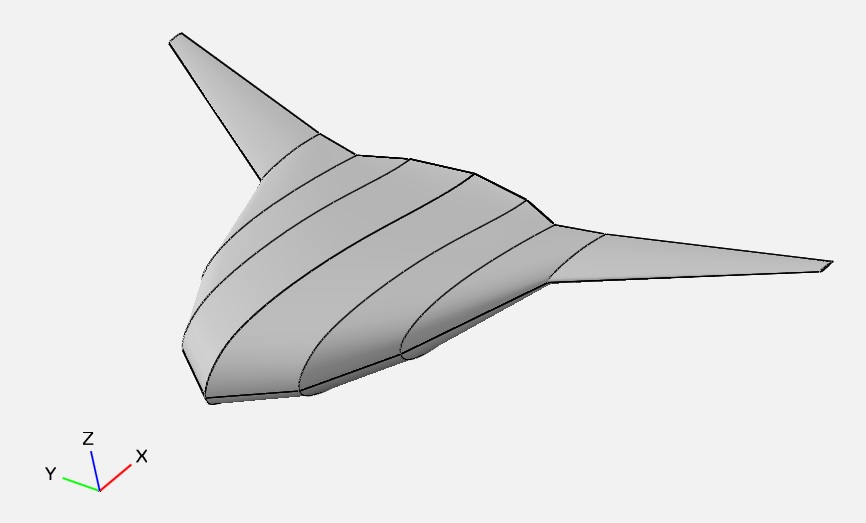
\includegraphics[keepaspectratio, width=\linewidth]{images/chap4/bwb_ref_geometry.jpg}
		\caption{Overall geometry.}
		\label{fig:bwb_ref_geom_overlook}
	\end{subfigure}
	\begin{subfigure}{0.4\textwidth}
		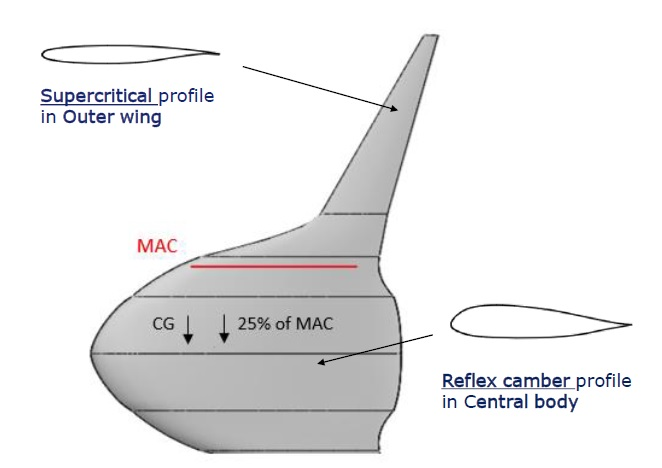
\includegraphics[keepaspectratio, width=0.9\linewidth]{images/chap4/bwb_ref_geometry_detail.jpg}
		\caption{Detail of geometry.}
		\label{fig:bwb_ref_geom_detail}
	\end{subfigure}
	\caption{ISAE-Supaero and ONERA Blended Wing-Body reference geometry.}
	\label{fig:bwb_ref_geometry}
\end{figure}

The TLAR of this reference geometry are the same of the Airbus A320, reported in Table~\ref{tab:bwb_ref_geometry_tlar}, together with some main parameters.
MTOW is estimated from the Breguet equation~\cite{bib:roskam_partI}, and it is just a first estimate that needs to be redefined later on.
\begin{table}[!h]
	\centering
	\begin{tabular}{l r l}
		\hline
		Number of passenger & 150 & \\
		Range & 2750 & nmi \\
		Cruise Mach & 0.78 & \\
		Aspect ratio & 5.37 & \\
		MTOW & 90.2 & \si{\tonne} \\
		Surface & 313 & \si{\square\meter} \\
		MAC & 9.68 & \si{\meter} \\
		Cruise altitude & 35000 & ft \\
		\hline
	\end{tabular}
	\caption{TLAR and main parameters for the ISAE-Supaero and ONERA Blended Wing-Body reference geometry.}
	\label{tab:bwb_ref_geometry_tlar}
\end{table}
It is to highlight that this geometry has not been optimised, but it is only a first reasonable configuration, used for studies and validation purposes.
Because of the lack of optimisation, it may be expected that the global efficiency will not be satisfying, but in this context these and other similar issues are not treated. 

\subsection{High fidelity aerodynamics study for the Blended Wing-Body}
\label{subsec:chap4_bwb_aero_cfd}

As remarked in the previous section, methods to estimate the $C_D$, described by Eq.~\eqref{eq:cd_total}, Eq.~\eqref{eq:cd0} and Eq.~\eqref{eq:cd_induced} may lose of validity.
The induced drag is derived by the lifting line theory, which is valid for small thickness-to-chord ratio and high aspect ratio. 
The first assumption may not be respected in the centerbody section, which has a relative thickness of about 15-18\%~\cite{bib:kozek}, the second instead is to verify since the BWB has intrinsecaly lower $AR$ than conventional aircraft.  
Wave drag is the hardest term to estimate, and the equation adopted is valid as far as the wing is not highly swept (below 25~\si{\deg}), whereas the BWB generally is very swept, especially in the center section. 

The CFD procedure is then adopted, to estimate each term and assess the error.
The software used is SU\textsuperscript{2}~\cite{bib:su2_main_paper, bib:su2_journal}, an open-source CFD code developed at Standford University. 
Unfortunately, it does not have its own mesher, requiring an external software for meshing purposes. 
At today, there is no big choice in meshing code, and most of them are commercial: in this research it has been used ICEM, belonging to the ANSYS repository~\cite{bib:ansys_pack}. 
The great advantage of ICEM is the O-Grid functionality, which allows to generate a good meshing around the body and decrease the cell size up to the far field, without losing the orthogonality of cells or the screwness~\cite{bib:cdn_notes}. 
For more details it is possible to refer to ANSYS manual guide.

Thanks to the O-grid feature, the number of cells is reduced: the final mesh for the BWB in real scale is made up of 8373239 cells; a detail of the meshing around the body is shown in Fig.~\ref{fig:bwb_mesh_detail}.
\begin{figure}[!h]
	\centering
	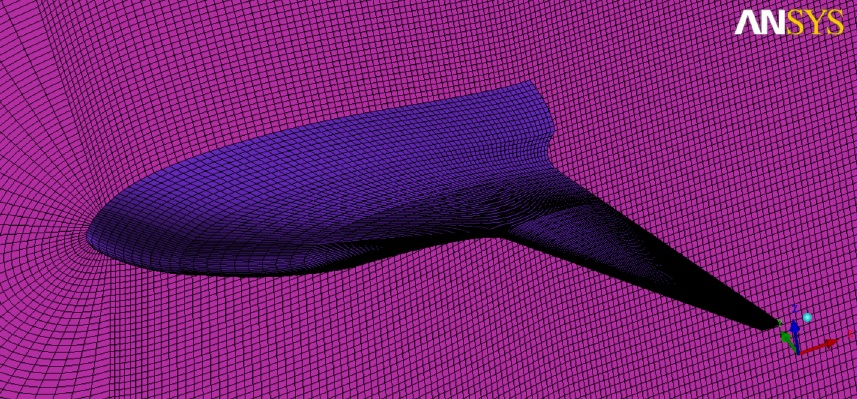
\includegraphics[keepaspectratio, width=0.6\textwidth]{images/chap4/bwb_mesh_detail.jpg}
	\caption{Detail of the Blended Wing-Body mesh around the body.}
	\label{fig:bwb_mesh_detail}
\end{figure}
Already at first sight, from Fig.~\ref{fig:bwb_mesh_detail} quality mesh can be appreciated. 
However, it is ensured checking that the screwness ratio tends to zero and the non-orthogonality is avoided. 
This last condition is critic particularly at the trailing edge, where sharp airfoil profiles make association with block a challenging task. 

The mesh is then given as input at SU\textsuperscript{2}, which converts it in a compatible format. 
The simulation is defined through a configuration file, since SU\textsuperscript{2} does not have a Graphical User Interface (GUI); within this file all the numerical and convective schemes must be defined. 
Of course, a unique choice does not exist, and a bad definition may strongly affect the convergence; the chosen simulation set-up is reported in Table~\ref{tab:bwb_cfd_setup}.
\begin{table}[!h]
	\centering
	\begin{tabular}{l c}
		\hline
		Mach & 0.78 \\
		Altitude & 35000~ft \\
		Model & RANS \\
		Turbulence model & Spalart-Allmaras \\
		Convective scheme & JST \\
		Limiter & Van Albada \\
		Spacial scheme & Grenn Gauss \\
		CFL number & 0.95 \\
		Linear solver & ILU \\
		\hline
	\end{tabular}
	\caption{Set up of CFD RANS simulations in SU2 for the BWB reference geometry aerodynamics study.}
	\label{tab:bwb_cfd_setup}
\end{table} 
The model is a fully turbulent RANS, which means that it includes all the terms of Navier-Stokes equations~\cite{bib:landau}: both the terms related to pressure and velocity field, mainly related to induced and compressibility term~\cite{bib:monti_pt1}, and the term related to the tensor stress which explains the viscous term~\cite{bib:monti_pt2}. 
The simulation point is the one corresponding to cruise; CFD schemes and solvers are chosen following the indication of classical CFD handbooks to ease the convergence~\cite{bib:ferziger_peric, bib:anderson_aero}. 
The turbulent Spalart-Allmaras is chosen because it is the most indicated for transonic regime~\cite{bib:pope}, limiter is considered to schematise the shock wave, which represents a discontinuity in the flow field~\cite{bib:leveque_conservation_laws}, and the CFL number is chosen close to 1 to facilitate the convergence~\cite{bib:leveque_partial_equation}.
The boundary conditions are of inlet/outlet at the far field and no-slip condition on the body: in that way, the velocity on the body is imposed to be zero, as comes out from the Prandtl theory for the boundary layer~\cite{bib:monti_pt2}. 
Other planes are of symmetry. 

Several points, at different angles of attack from -3 to 10~\si{\deg}, are evaluated; results are compared with the polars obtained in FAST, and with VSPAero, a suite included in OpenVSP to compute aerodynamics using a Vortex-Lattice method (VLM).
For the convergence, the residuals are studied: if the main force parameters $C_L$, $C_D$ and $C_M$ reach a constant value with a given tolerance, the simulation is considered over and converged.
Among the three, the most critic coefficient is $C_D$, since to have an accurate estimation a tolerance of $10^{-6}$ is needed.
An example of CFD history is given in Fig.~\ref{fig:cfd_conv_history}.
\begin{figure}[!h]
	\centering
	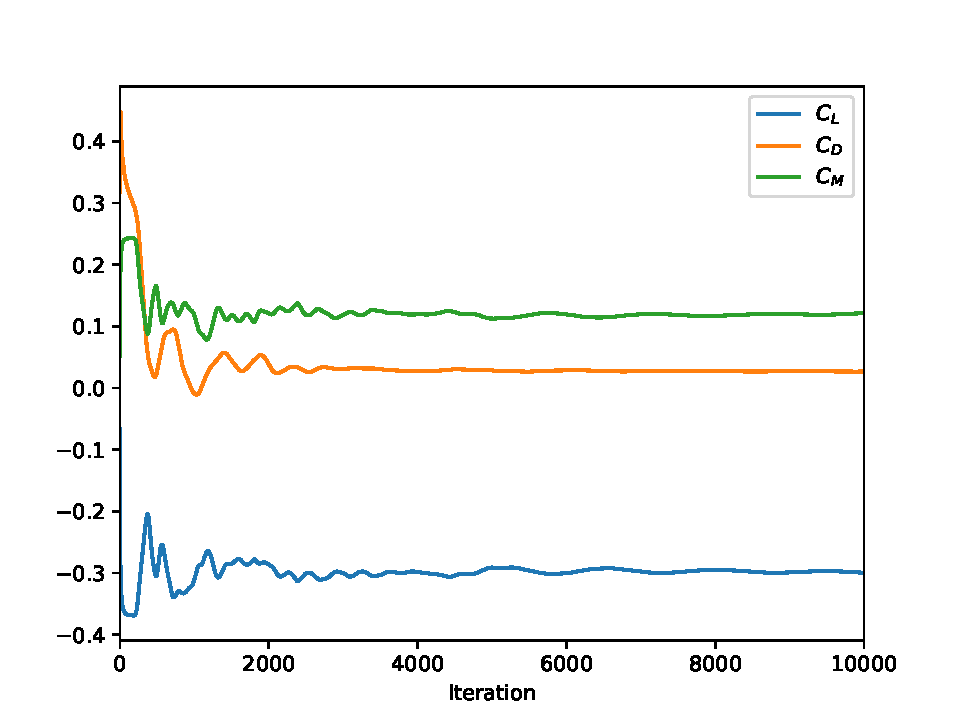
\includegraphics[keepaspectratio, width=0.6\textwidth]{images/chap4/cfd_hist_example}
	\caption{Convergence history example for CFD simulation, $\alpha$=-3~\si{\deg}, M=0.78 and h=35000~ft.}
	\label{fig:cfd_conv_history}
\end{figure}

First curve presented is the $C_L-\alpha$, shown in Fig.~\ref{fig:cl_alpha_rans}.
\begin{figure}[!h]
	\centering
	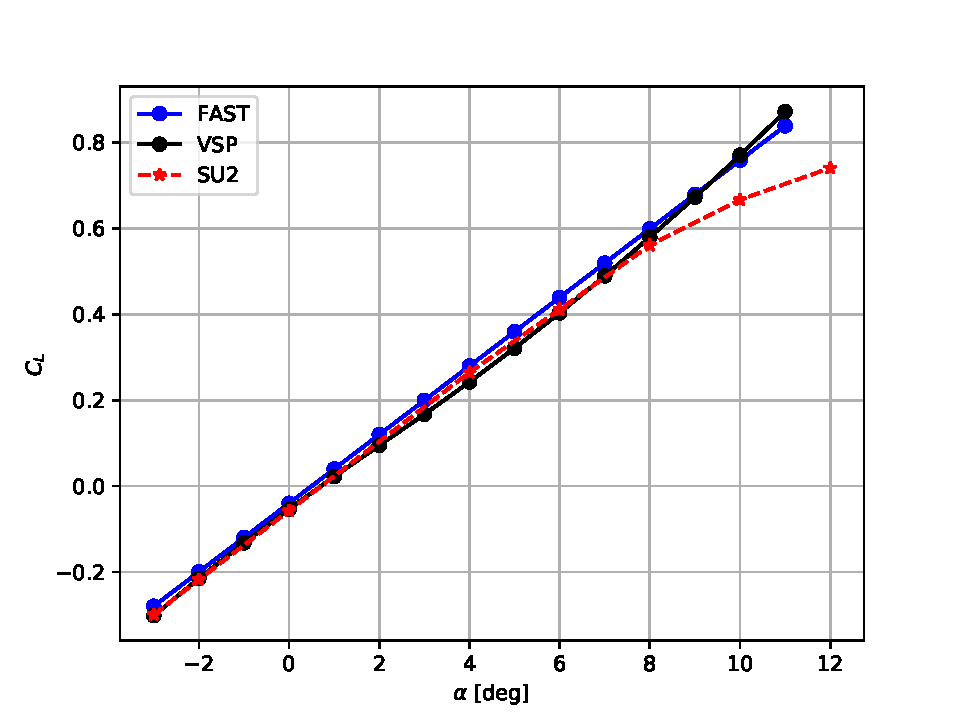
\includegraphics[keepaspectratio, width=0.6\textwidth]{images/chap4/cl_alpha_rans}
	\caption{$C_L-\alpha$ curve, comparison between SU2, FAST and OpenVSP. RANS simulation case, M=0.78 and h=35000~ft.}
	\label{fig:cl_alpha_rans}
\end{figure}
Visually, it can be seen that FAST, VSP and SU\textsuperscript{2} are in good agreement in the linear zone, then at high angle of attack both FAST and VSP still show a linear trend, whereas SU2 captures the stall. 
This is expected since in FAST the curve is obtained simply as a straigth line from the estimation of the slope $C_{L_{\alpha}}$ using the result from lifting line, and VSP uses a VLM method which has in its limitation the non viscous flow hypothesis. 
However, for the cruise the most interesting zone is the linear one, and in this region no corrections are needed. 
This is also confirmed having a look at the values of the slope $C_{L_{\alpha}}$ reported in Table~\ref{tab:cla_rans_comparison}: both of them slightly overestimate the value of SU2, but the difference is within the 1\%, that is acceptable at this stage. 
\begin{table}[!h]
	\centering
	\begin{tabular}{l c}
		\hline
		SU2 & 4.575~\si{\per\radian} \\ 
		VSP & 4.649~\si{\per\radian} \\
		FAST & 4.578~\si{\per\radian} \\
		\hline
	\end{tabular}
	\caption{Comparison of the slope $C_{L_{\alpha}}$ estimated by SU2, VSP and FAST. RANS simulation case, M=0.78 and h=35000~ft.}
	\label{tab:cla_rans_comparison}
\end{table}

The second curve shown is the polar $C_L-C_D$, depicted in Fig.~\ref{fig:clcd_rans}. 
\begin{figure}[!h]
	\centering
	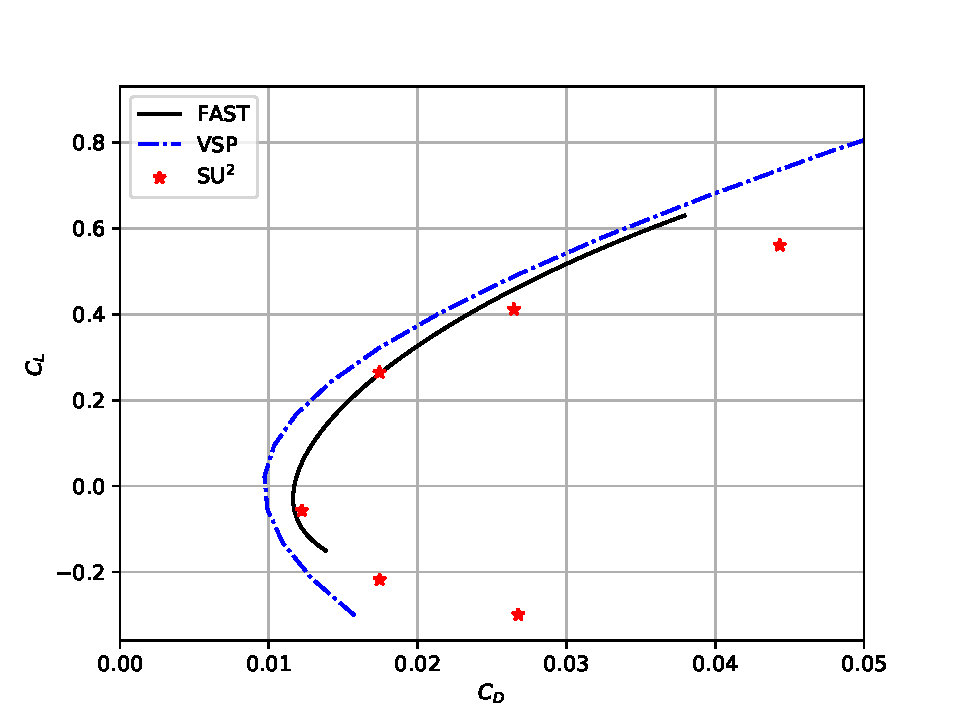
\includegraphics[keepaspectratio, width=0.6\textwidth]{images/chap4/clcd_rans}
	\caption{$C_D-C_L$ curve, comparison between SU2, FAST and OpenVSP. RANS simulation case M=0.78 and h=35000ft.}
	\label{fig:clcd_rans}
\end{figure}
Contrarily to the previous case, here the three methods show differences. 
The first to note is that the VSP curve is shifted on the left, which means that the term $C_{D_{0}}$ is underestimated. 
FAST and SU2 present instead a good agreement, still in the zone of low $C_L$; at higher values SU2 estimates a drag coefficient much higher. 
Having assessed that $C_{D_{0}}$ matches for both cases, the other two terms cause this divergence. 
Table~\ref{tab:oswald_comparison} reports the values for the Oswald coefficient: for all the three methods there is a good match (maximum error is still below 2\%). 
Since the parameter $e$ is the same, the term $C_{D_{i}}$ matches too. Indeed, from Eq.~\eqref{eq:cd_induced} the only parameter that may vary is $e$.
\begin{table}[!h]
	\centering
	\begin{tabular}{l c}
		\hline
		SU\textsuperscript{2} & 0.986 \\ 
		OpenVSP & 0.992 \\
		FAST & 0.987 \\
		\hline
	\end{tabular}
	\caption{Comparison of the Oswald coefficient $e$, estimated by SU2, FAST and OpenVSP. RANS simulation case. M=0.78 and h=35000~ft.}
	\label{tab:oswald_comparison}
\end{table} 
As a conclusion, the drag divergence in SU2 is caused by the wave drag term: it seems that FAST and OpenVSP underestimate this term. 
This is expected in OpenVSP, since the VLM is valid only in subsonic flow; as far as FAST is concerned, it means that the method used can be applied to conventional aircraft but loses its validity for a BWB, mainly because of the highly swept configuration. 

It is to mention that an Oswald coefficient near 1 confirms that the BWB is efficient from an aerodynamics point of view, since $e=1$ corresponds to the optimal lift distribution. 
A BWB configuration is a low aspect ratio, and indeed the Jones theory for delta wing is more accurate than the Prandtl theory~\cite{bib:cdn_notes}. 
This theory forecasts an elliptical distribution, which is confirmed by the Oswald coefficient; in fact $e=1$ coincides with elliptical distribution~\cite{bib:anderson_aero}.

For completeness, the efficiency curve is shown in Fig.~\ref{fig:l2d_rans}, where the LoD value drops off above $C_L=0.5$ approximately. 
\begin{figure}[!h]
	\centering
	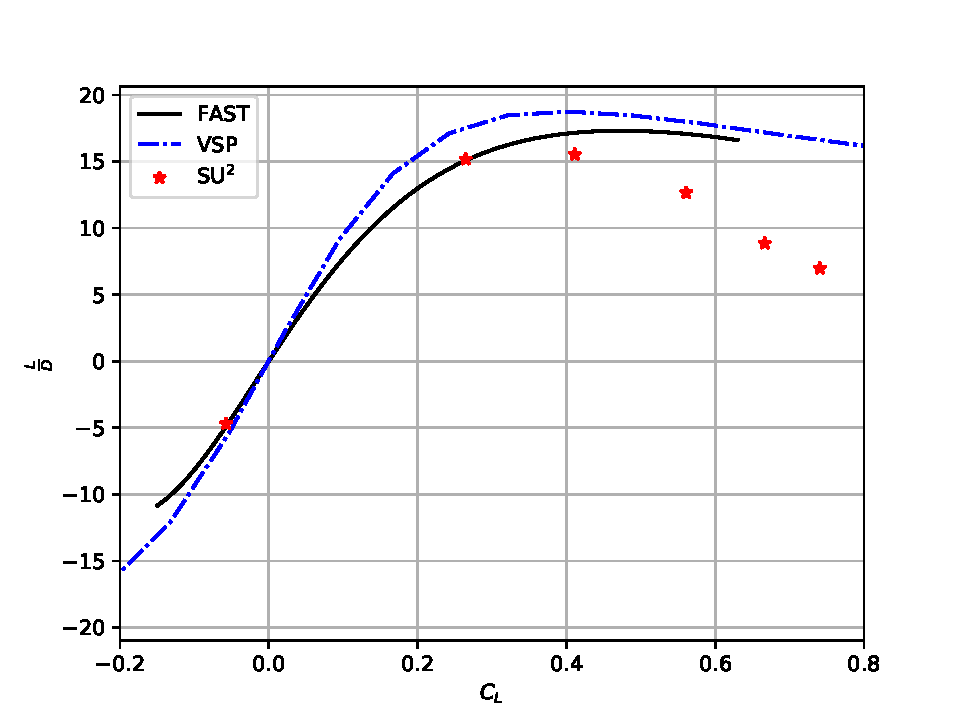
\includegraphics[keepaspectratio, width=0.6\textwidth]{images/chap4/l2d_rans}
	\caption{Lift-over-drag ratio curve, comparison between SU2, FAST and OpenVSP. RANS simulation case. M=0.78 and h=35000~ft.}
	\label{fig:l2d_rans}
\end{figure}
Note that the maximum LoD value is around 17-18: as stated at the beginning, the reference geometry is just a first estimate and has not been optimised to maximise the aerodynamics; however this issue is not addressed since for validation purposes only a comparison is of interest. 
Also, the optimum $C_L$ is approximately 0.4, which is high for a BWB, pheraps this suggests that the initial estimate of 35000~ft as cruise altitude must be revised. 

Finally, a latest analysis is done to estimate the Mach divergence, defined as the Mach number starting from which the following condition is satisfied:
\begin{equation}
	\label{eq:mach_divergence}
	\frac{\textrm{d}C_D}{\textrm{d}M}=0.1
\end{equation}

The analysis is conducted varying the Mach number at a given angle of attack, $\alpha$=1.5~\si{\deg}. 
Results are shown in Fig.~\ref{fig:mach_drag_div}: at low $\alpha$ the drag coefficient is almost constant, because the wave drag is near zero, but it start to diverge as soon as the transonic regime starts. 
The Mach divergence is marked in black and is equal to 0.803, so very close to the Mach design.
This is not a favorable condition, and a further redesign may be done. 
\begin{figure}[!h]
	\centering
	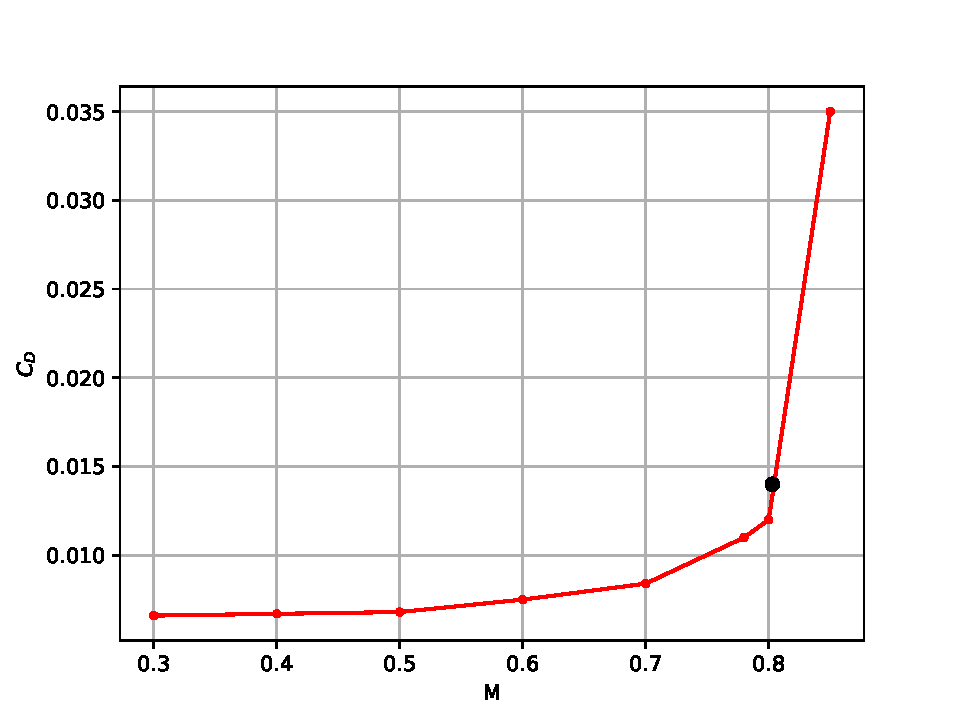
\includegraphics[keepaspectratio, width=0.6\textwidth]{images/chap4/mach_divergence_euler}
	\caption{$C_D-M$ curve, $\alpha$=1.5~\si{\deg} and h=35000~ft. Drag divergence point marked in black.}
	\label{fig:mach_drag_div}
\end{figure}
The results from Fig.~\ref{fig:mach_drag_div} state also that in low speed, when the wave drag is not relevant, a good agreement between low and high fidelity methods is expected, since it has already been shown that the induced drag estimation works well. 

To conclude, this analysis shows that methods used in FAST still maintain their validity for the estimation of $C_{D_{0}}$ and $C_{D_{i}}$ terms, but the compressibility model fails. 
Thus the equation has been recalibrated, including a corrective term to match the results from high-fidelity. 
Also, from the CFD simulations the parameters $C_{L_{\alpha}}$ and $C_{M_{\alpha}}$ are estimated.
From their knowledge it is possible to compute the static margin as~\cite{bib:anderson_perfo}
\begin{equation}
	\label{eq:static_margin_perfo}
	SM = -\frac{C_{M_{\alpha}}}{C_{L_{\alpha}}}
\end{equation}
The application of Eq.~\eqref{eq:static_margin_perfo} yields to $SM=0.46$, which is out of the allowable domain of 5 and 10\% of the MAC.
This may result in some difficulties to stabilize the aircraft. 

This point will be addressed in next section, that reports the sizing of control surfaces for the longitudinal control. 

\subsection{Control surfaces sizing for the BWB longitudinal control}
\label{subsec:chap4_bwb_control}

\subsubsection{The control problem formulation}
\label{subsubsec:chap4_bwb_control_prob_formulation}

This section is deputed to the study of control surfaces sizing for a BWB, focusing on the problem of the longitudinal control. 
The control discipline is not directly included in FAST, at this stage, but several work in literature markes the BWB control as a priority for its design~\cite{bib:nickel, bib:kozek, bib:perry, bib:wang, bib:ashkenas}, and so it has been decided to carry out the design of control surfaces, for the longitudinal control, in order to understand if the concept can be trimmed in some way. 
In case of negative answer, there is no need to proceed with further sizing investigation. 

At first order, considering small angles, longitudinal equations are decoupled from the lateral ones, and it is then possible to semplify the equations considering only the simmetry plane~\cite{bib:roskam_flight_dynamics}. 
The longitudinal flight dynamics equations are reported below, with the notation that follows the scheme of Fig.~\ref{fig:aircraft_flight_dynamics_scheme}~\cite{bib:kuethe, bib:agodemar_dsv}; the momentum is considered positive when it is pitching up.
\begin{equation}
	\label{eq:flight_dynamics_system}
	\left\{\begin{array}{l}
		m\dot{V} = -\frac{1}{2}\rho V^2 S_w C_D + T - mg\gamma \\
		mV\dot{\gamma} = \frac{1}{2}\rho V^2 S_w C_L -mg \\
		I_{yy}\dot{q} = \frac{1}{2}\rho V^2 S_w \bar{c} C_{M_{cg}} \\
		\dot{q} = \dot{\alpha} + \dot{\gamma}
	\end{array}\right.
\end{equation}
In Eq.~\eqref{eq:flight_dynamics_system}, $m$ represents the mass, $\alpha$ the angle of attack, $\gamma$ the flight path angle, $V$ the velocity, $I_{yy}$ the inertial momentum along the $y$-axis, $q$ the angular speed and the dot represents the derivative with respect to time. 
\begin{figure}[!h]
	\centering
	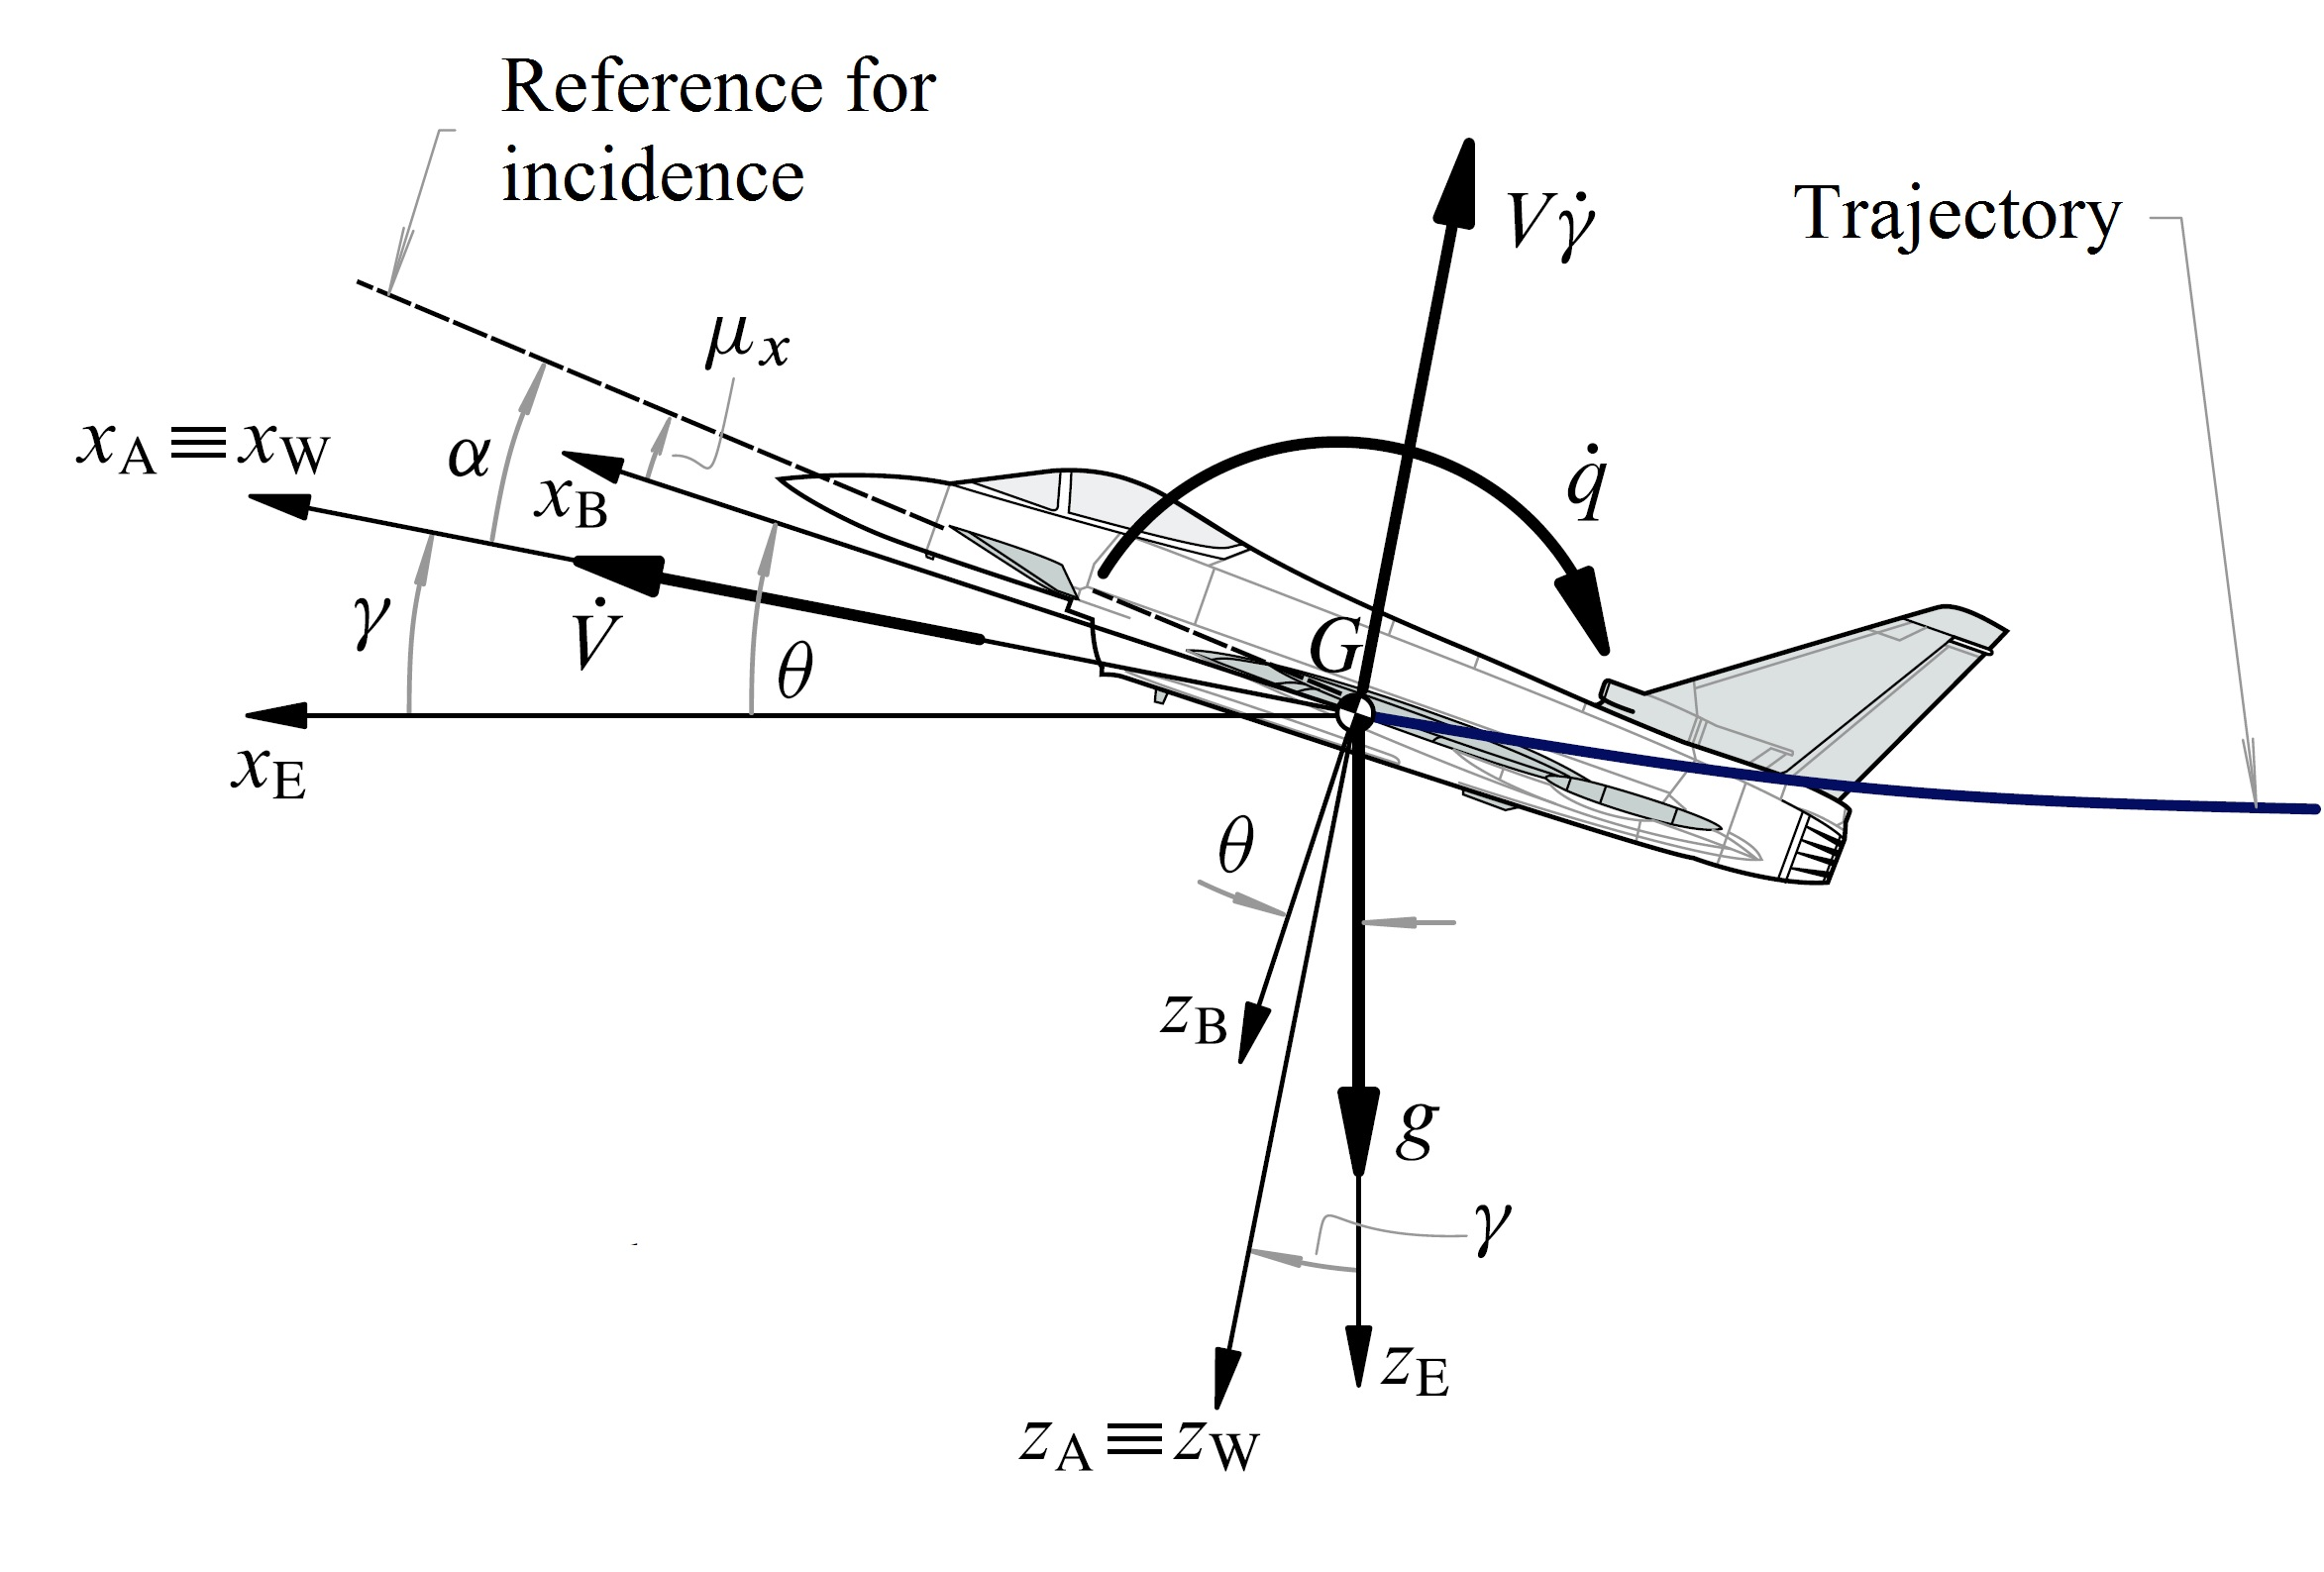
\includegraphics[keepaspectratio, width=0.6\textwidth]{images/chap4/aircraft_flight_dynamics_scheme.jpg}
	\caption{Aircraft diagram scheme, noting the angle of attack $\alpha$, the flight path angle $\gamma$ and the line for indices~\cite{bib:agodemar_dsv}.}
	\label{fig:aircraft_flight_dynamics_scheme}
\end{figure}

To close the problem, an aerodynamics model for the computation of $C_L$, $C_D$ and $C_{M_{cg}}$ needs to be defined. 
In the hypothesis of small angle of attack, it is possible to define some linear relations as follow:
\begin{equation}
	\label{eq:aero_model_flight_dynamics}
	\left\{\begin{array}{l}
		C_L = C_{L_{0}} + C_{L_{\alpha}}\alpha + C_{L_{q}} \frac{q}{\bar{c}{V}} + C_{L_{\delta_{e}}}\delta_{e} \\
		C_D = C_{D_{0}} + k C_L^2 + C_{D_{w}} \\
		C_M = C_{M_{0}} + C_{M_{\alpha}}\alpha + C_{M_{q}} \frac{q}{\bar{c}{V}} + C_{M_{\delta_{e}}}\delta_{e} 
	\end{array}\right.
\end{equation}

Beside the already known parameters, such as $C_{L_{\alpha}}$ and $C_{M_{\alpha}}$, new quantities appear: $\delta_{e}$ is the deflection of control surfaces, $C_{L_{q}}$ and $C_{L_{\delta_{e}}}$ are the slope of $C_L$ with respect to a variation of $q$ and $\delta_{e}$. 
$C_{M_{q}}$ and $C_{M_{\delta_{e}}}$ have a similar meaning, referring to momentum coefficient $C_M$. 
Note that $C_M$ must be computed around the center of gravity, to have coherency with the set of Eq~\eqref{eq:flight_dynamics_system}. 
Finally, $k$ is computed from Eq.~\eqref{eq:cd_induced}.

Combining Eq.~\eqref{eq:aero_model_flight_dynamics} with Eq.~\eqref{eq:flight_dynamics_system}, it is possible to linearize the flight dynamics equations. 
For brevity, this system of equations can be written in matrix form in the state space~\cite{bib:kuethe}:
\begin{equation}
	\label{eq:flight_dynamics_state_space}
	\left\{ \begin{array}{l}
		\dot{\underline{x}} = \mathbf{A}\underline{x} + \mathbf{B}\underline{u} \\
		\underline{y} = \mathbf{C}\underline{x}
		\end{array} \right .
\end{equation}
where $\underline{x}$ is the state vector, that includes the entries the pitch rate $q$ and the small variations of $V$, $\alpha$ and $\gamma$, $\underline{y}$ is the output vector, including also the load factor $n$~\cite{bib:megson}, $\underline{u}$ the control vector, which includes only the entry $\delta_{e}$, and $\mathbf{A}$, $\mathbf{B}$ and $\mathbf{C}$ are three matrices. 
The formulation of Eq.~\eqref{eq:flight_dynamics_state_space} is easier to manipulate in a simulation system like Matlab/Simulink~\cite{bib:simulink}, that will be used later. 

At this point, for the BWB reference geometry only $C_{L_{0}}$, $C_{M_{0}}$, $C_{L_{\alpha}}$ and $C_{M_{\alpha}}$ are known from the CFD results of Sec.~\ref{subsec:chap4_bwb_aero_cfd}; the others must be estimated. 
$C_{L_{q}}$ and $C_{M_{q}}$ depend solely on the geometry meanwhile $C_{L_{\delta_{e}}}$ and $C_{M_{\delta_{e}}}$ depend also on the control surfaces definition, then an assumption on their placement must be done. 

Table~\ref{tab:overall_param_bwb_flight_dyn} reports the overall coefficients for the analysis to be conducted: the Mach is set to 0.3, and so the case is the low speed one; indeed the control surfaces must equilibrate the momentum coefficient at low speed, Mach close to takeoff and sea level.
In real the aircraft must be trimmed at maximum $C_L$, but the objective is not achievable without a level of refinement that includes a full RANS model, and thus the flight domain is limited to the equilibrium point. 
The next improvement will be to enlarge this study at high lift, considering also the dutch-roll. 
\begin{table}[!h]
	\centering
	\begin{tabular}{l r l}
		\hline
		M & 0.3 & \\
		$I_{yy}$ & 11165 & \si{\kilogram\square\meter} \\
		$C_{L_{\alpha}}$ & 4.47 & \si{\per\radian} \\
		$C_{M_{\alpha}}$ & - 2.06 & \si{\per\radian} \\
		$C_{L_{q}}$ & 0.79 & \si{\per\radian} \\
		$C_{M_{q}}$ & -0.88 & \si{\per\radian} \\
		\hline
	\end{tabular}
	\caption{Geometrical and aerodynamics coefficients for the BWB reference geometry, for longitudinal control surface purposes.}
	\label{tab:overall_param_bwb_flight_dyn}
\end{table}

The slope $C_{L_{\alpha}}$ and $C_{M_{\alpha}}$ come from CFD simulations at $M=0.3$; note that only 2 points in the linear zone are necessary for their estimation.
The terms $C_{L_{q}}$ and $C_{M_{q}}$, instead are computed using VLM method of AVL~\cite{bib:avl} and classical relations from Roskam~\cite{bib:roskam_flight_dynamics}. 
The inertial parameter $I_{yy}$ is given by OpenVSP.
It is to highlight that the procedure here is multifidelity, since it uses both CFD and VLM results.

Concerning the control surfaces placement, the work already done by Denieul has been used as reference~\cite{bib:denieul}.
The BWB is a tailless configuration, and then the idea of using a single control surfaces as ailerons and elevators arises; to stress their double capacity they are called generically ``elevons''. 
Six different configurations have been considered, reported in Fig.~\ref{fig:bwb_elevon_configuration}, they are made up using just three basic elevon configurations:
\begin{itemize}
	\item Type A, in the centerbody;
	\item Type B, in the inboard external wing;
	\item Type C, in the outboard external wing. 
\end{itemize}
\begin{figure}[!h]
	\centering
	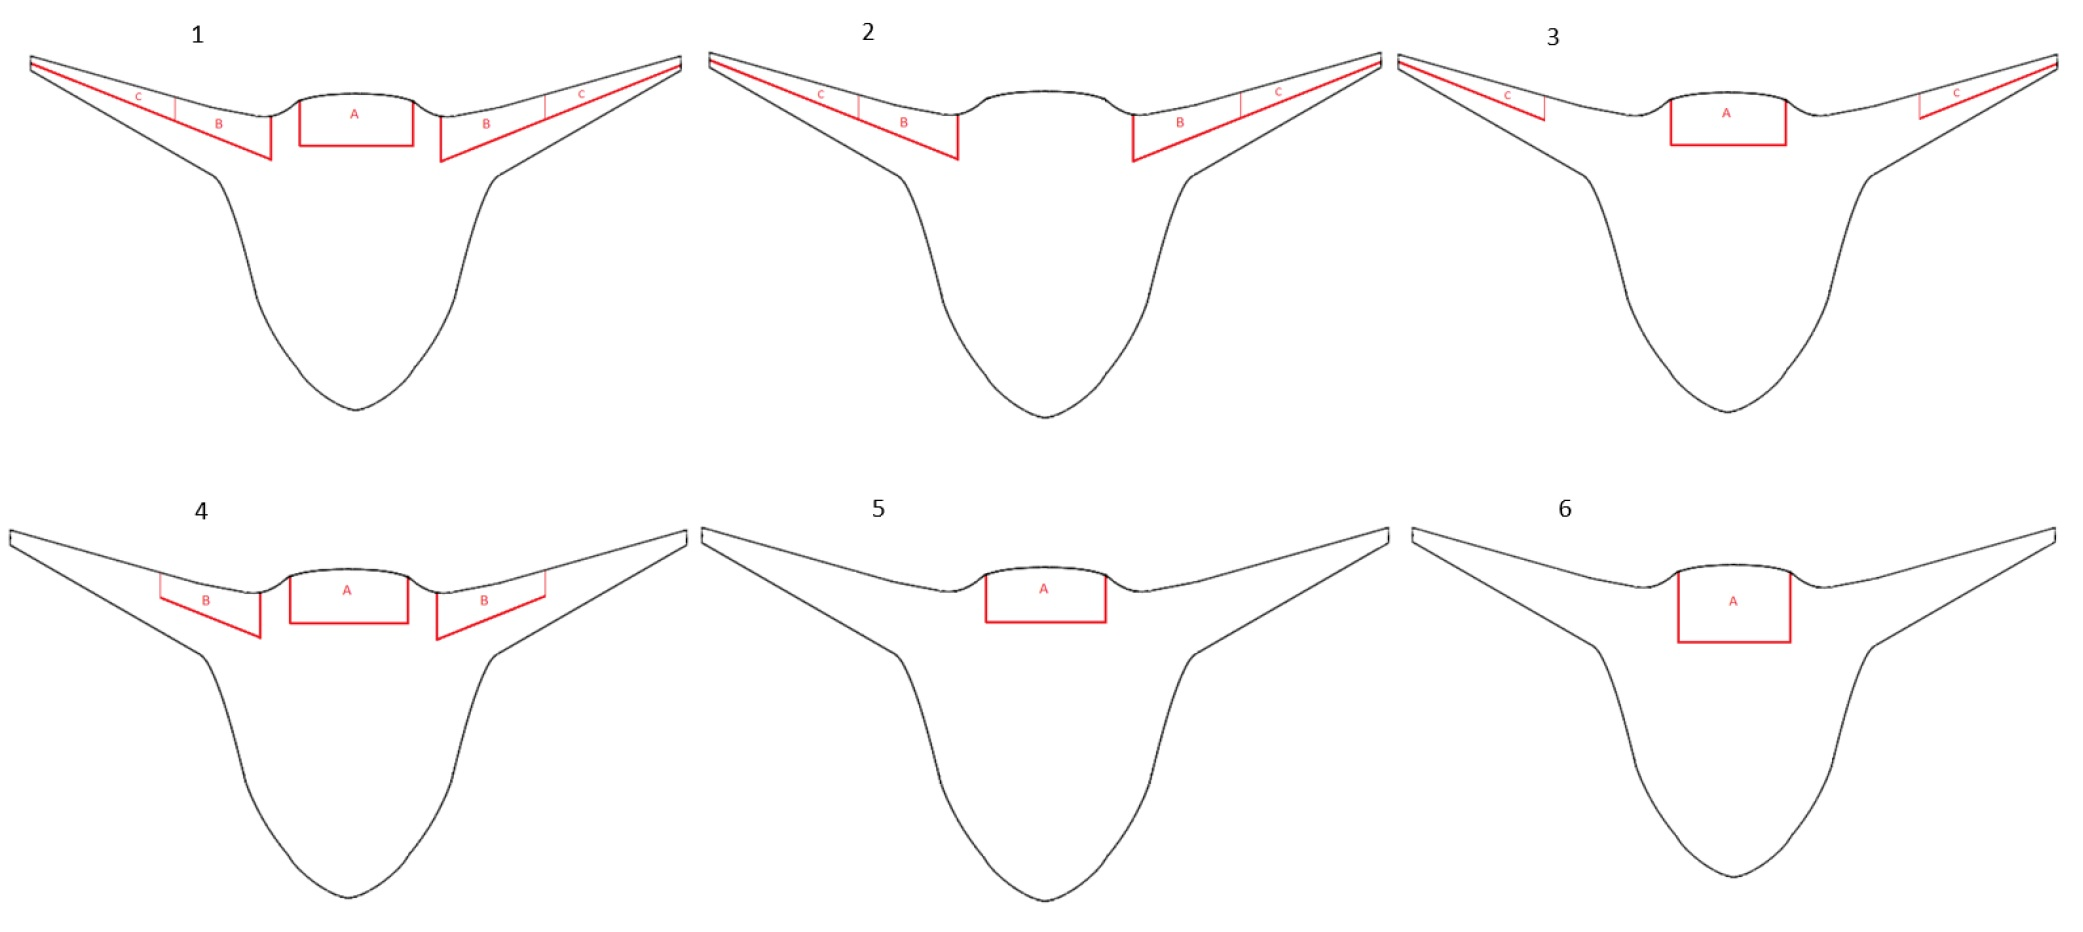
\includegraphics[keepaspectratio, width=\textwidth]{images/chap4/bwb_elevons_configuration.jpg}
	\caption{The 6 control surfaces configurations proposed for the BWB reference geometry for the purpose of this research activity.}
	\label{fig:bwb_elevon_configuration}
\end{figure}

The coefficients $C_{L_{\delta_{e}}}$ and $C_{M_{\delta_{e}}}$ are estimated considering VLM method and relations from Roskam book.
Table~\ref{tab:aero_coeff_elevon_conf} reports the value of these coefficients for each configuration. 
These coefficients can be also seen as efficiency; the bigger are (in absolute value), the less deflection is needed for a given maneuveur.
\begin{table}[!h]
	\centering
	\begin{tabular}{l l c c c c c c}
		\cline{3-8}
		& & \multicolumn{6}{c}{Configuration} \\
		& & 1 & 2 & 3 & 4 & 5 & 6 \\
		\hline
		$C_{L_{\delta_{e}}}$ & [\si{\per\radian}] & 1.87 & 1.33 & 1.18 & 1.28 & 0.56 & 0.73 \\
		$C_{M_{\delta_{e}}}$ & [\si{\per\radian}] & -1.61 & -1.18 & -1.05 & -0.98 & -0.42 & -0.49 \\
		\hline
	\end{tabular}
	\caption{$C_{L_{\delta_{e}}}$ and $C_{M_{\delta_{e}}}$ coefficients for the 6 configurations shown in Fig.~\ref{fig:bwb_elevon_configuration}. They are computed using VLM technique~\cite{bib:avl}.}
	\label{tab:aero_coeff_elevon_conf}
\end{table}

Other important coefficient to evaluate is the hinge moment for control surfaces, defined as
\begin{equation}
	\label{eq:hinge_moment_def}
	\mathcal{M}_H = \frac{1}{2}\rho S_H c_H V^2 C_H
\end{equation}
where $H$ is the hinge moment and $C_H$ the relative coefficient, $S_H$ and $c_H$ the reference area and length respectively for elevons. 
The hinge moment coefficient is modeled in a similar manner than the other aerodynamics coefficient: 
\begin{equation}
	\label{eq:hinge_moment_coeff_model}
	C_H = C_{H_{0}} + C_{H_{\alpha}}\alpha + C_{H_{\delta_{e}}}\delta_{e}
\end{equation}

The coefficients that appear in Eq.~\eqref{eq:hinge_moment_coeff_model} are estimated directly in AVL; results for each configuration are reported in Table~\ref{tab:hinge_coeff_elevon_conf}.
\begin{table}
	\centering
	\begin{tabular}{l l c c c c c c}
		\cline{3-8}
		& & \multicolumn{6}{c}{Configuration} \\
		& & 1 & 2 & 3 & 4 & 5 & 6 \\
		\hline
		$C_{H_{0}}$ & & 0.002558 & 0.003074 & 0.001205 & 0.000801 & -0.000516 & -0.002178 \\
		$C_{H_{\alpha}}$ & [\si{\per\radian}] & 0.019881 & 0.017334 & 0.009186 & 0.012827 & 0.002598 & 0.011336 \\
		$C_{H_{\delta_{e}}}$ & [\si{\per\radian}] & 0.032088 & 0.019938 & 0.015927 & 0.020709 & 0.008863 & 0.021461 \\
		\hline
	\end{tabular}
	\caption{Hinge moment coefficients to define the model of Eq.~\eqref{eq:hinge_moment_coeff_model} for the 6 different configurations shown in Fig.~\ref{fig:bwb_elevon_configuration}.}
	\label{tab:hinge_coeff_elevon_conf}
\end{table}

\subsubsection{The longitudinal control for a BWB configuration}
\label{subsubsec:chap4_bwb_longitudinal_control_results}

In order to draw conclusions, a closed loop control law is modeled in Matlab/Simulink~\cite{bib:simulink}; the problem is solved using the $H_{\infty}$ technique~\cite{bib:apkarian}.
The thrust effects are neglected in this analysis, thus relative terms in Eq.~\eqref{eq:flight_dynamics_system} are set to zero. 

Four different criteria are considered to evaluate performances of the configurations: the hinge moment coefficient evaluation, the saturation limits (defined by the maximum load factor in the flight envelope, for the category chosen $n=2.5$~\cite{bib:megson}), the surface deflection and the power demand for the elevons actuation, defined as~\cite{bib:fraj}
\begin{equation}
	\label{eq:actuator_power_demand}
	P_{act}\left(t\right) = \dot{\delta}_{e}\left(t\right)\mathcal{M}_{H}\left(t\right)
\end{equation}

These quantities are evaluated for each configuration shown in Fig.~\ref{fig:bwb_elevon_configuration}, on a given set of angles of attack. 
Results are shown in Fig.~\ref{fig:bwb_control_elevon_deflection} for the elevon deflection, Fig.~\ref{fig:bwb_control_hinge_moment} for the maximum hinge moment and Fig.~\ref{fig:bwb_control_peak_power} for the actuator peak power. 
\begin{figure}[!h]
	\centering
	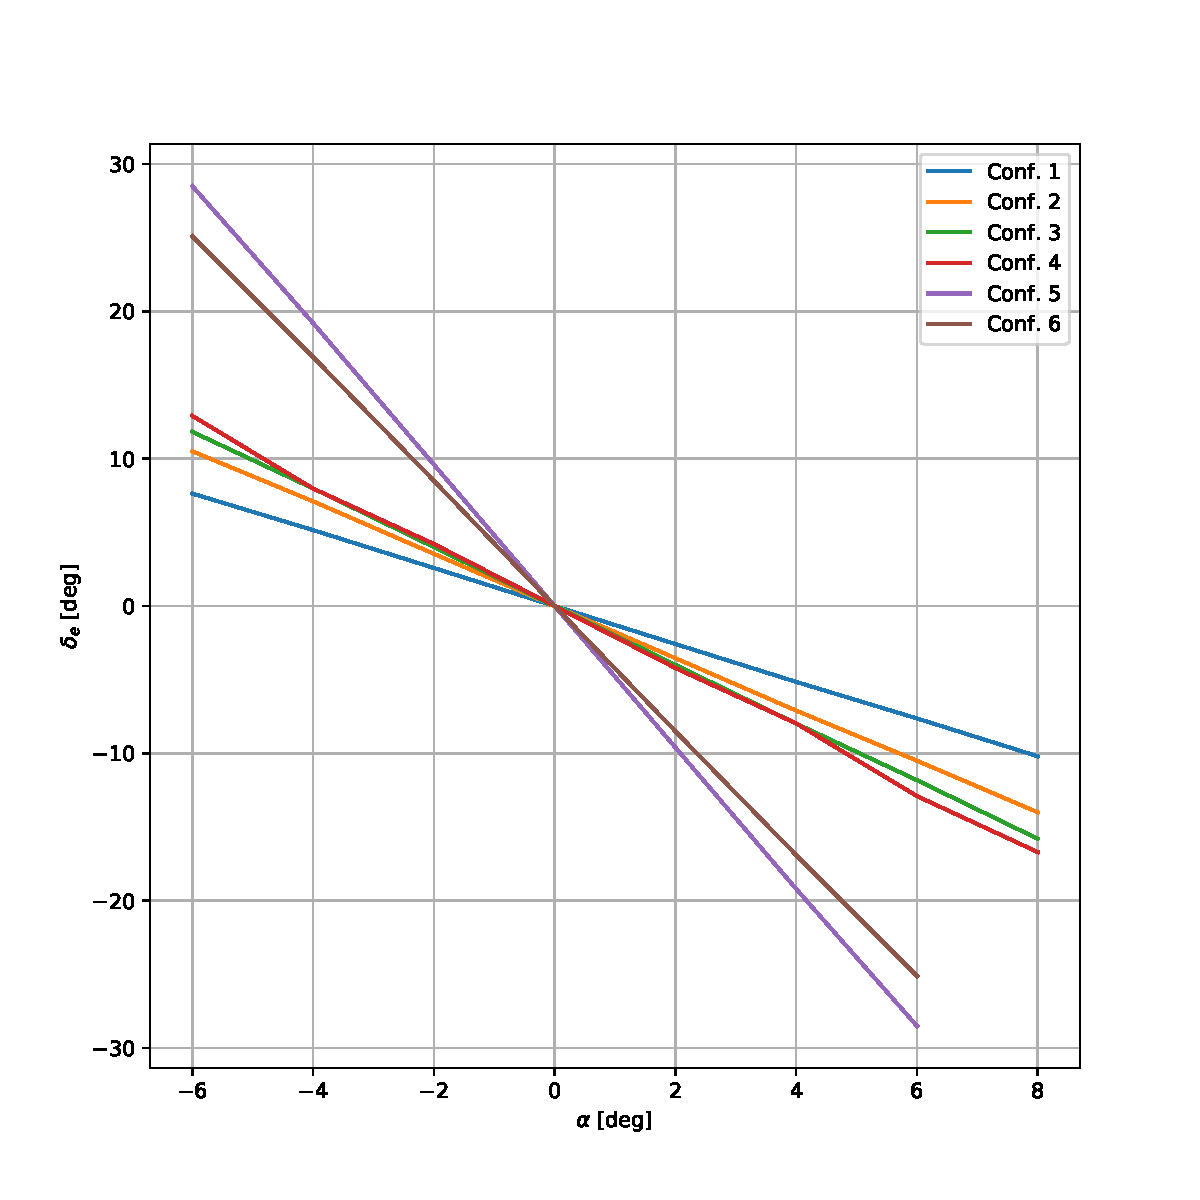
\includegraphics[keepaspectratio, width=0.6\textwidth]{images/chap4/bwb_control_elevon_deflection}
	\caption{Elevon deflection $\delta_{e}$ for the 6 BWB configurations of Fig.~\ref{fig:bwb_elevon_configuration}, as function of demanded angle of attack.}
	\label{fig:bwb_control_elevon_deflection}
\end{figure}
\begin{figure}[!h]
	\centering
	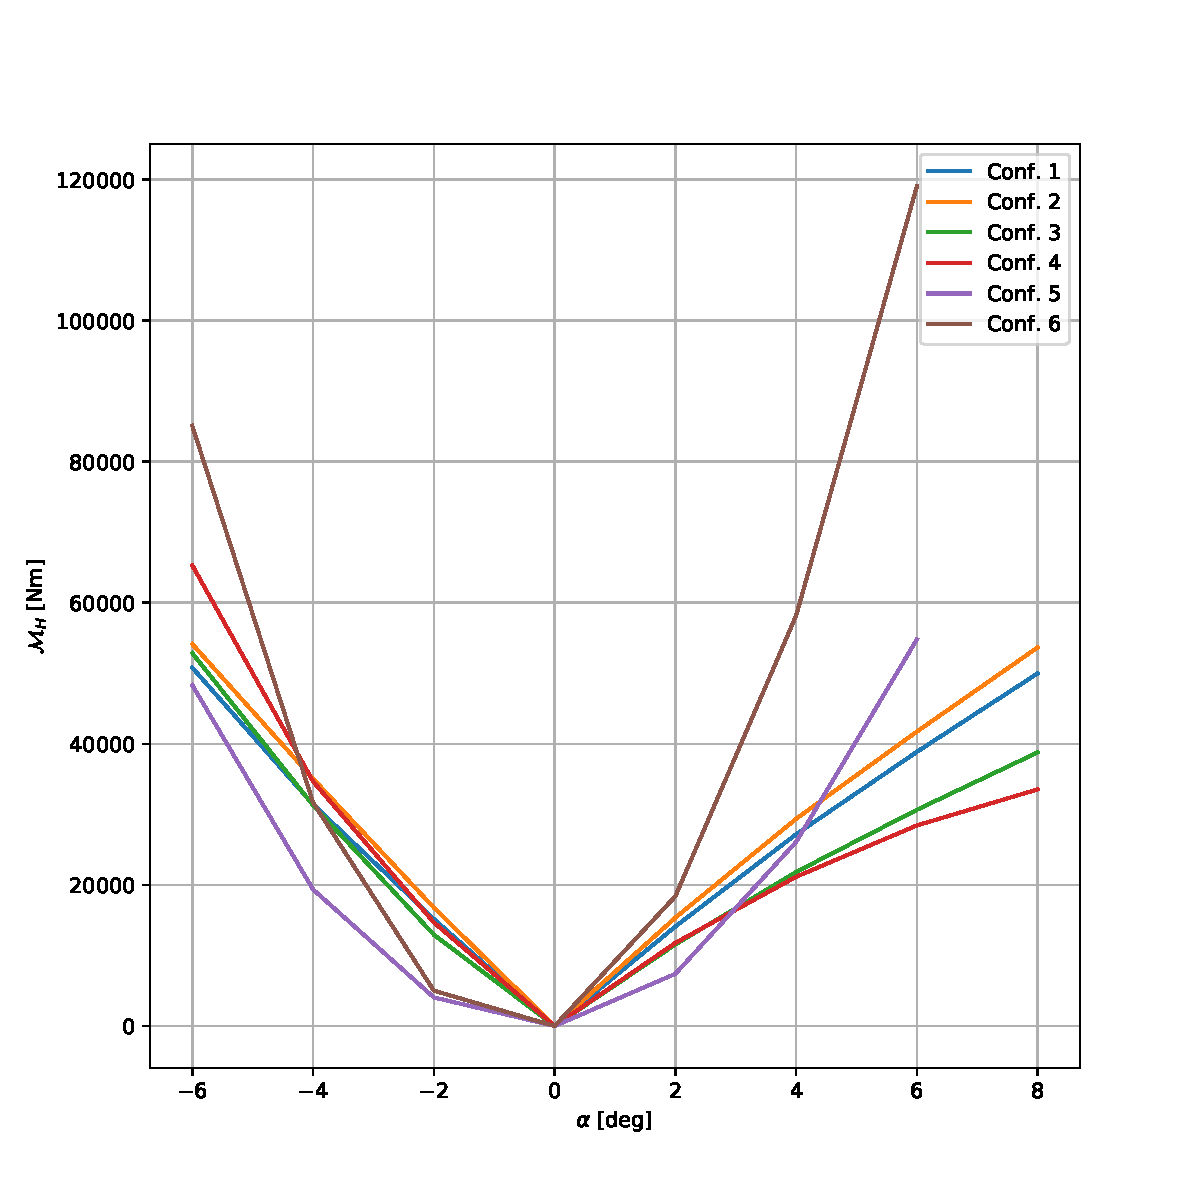
\includegraphics[keepaspectratio, width=0.6\textwidth]{images/chap4/bwb_control_hinge_moment}
	\caption{Maximum hinge moment for the 6 BWB configurations of Fig.~\ref{fig:bwb_elevon_configuration}, as function of demanded angle of attack.}
	\label{fig:bwb_control_hinge_moment}
\end{figure}
\begin{figure}[!h]
	\centering
	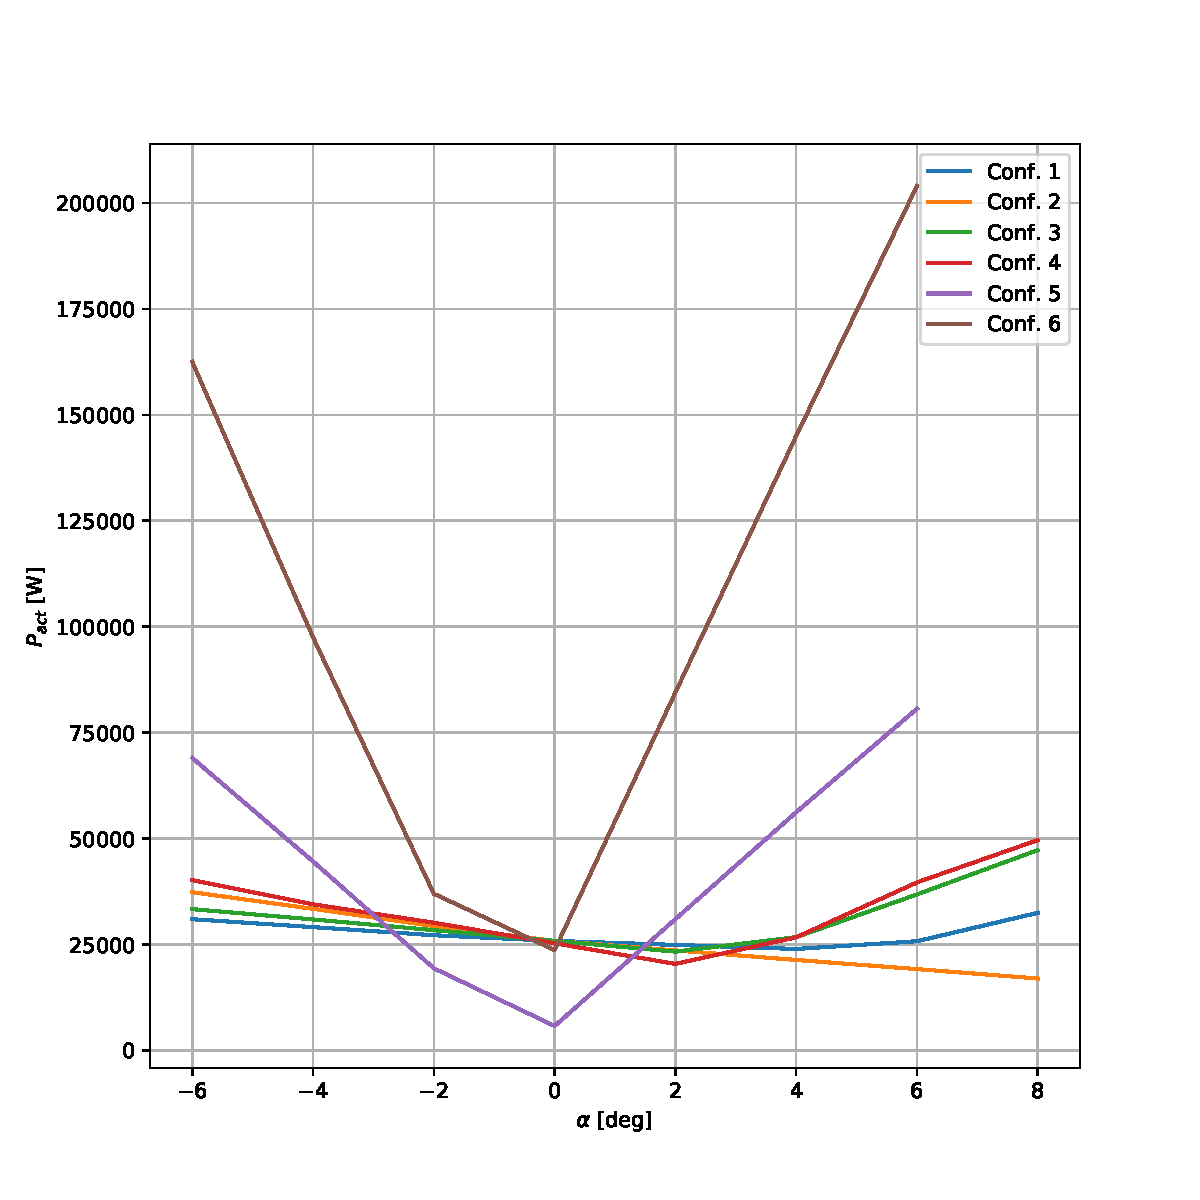
\includegraphics[keepaspectratio, width=0.6\textwidth]{images/chap4/bwb_control_peak_power}
	\caption{Peak power for the 6 BWB configurations of Fig.~\ref{fig:bwb_elevon_configuration}, as function of demanded angle of attack.}
	\label{fig:bwb_control_peak_power}
\end{figure}

In terms of elevons deflection (Fig.~\ref{fig:bwb_control_elevon_deflection}), the first configuration is indeed the one that gives the best results, especially for high variations of angle of attack (which are equivalent to high load factors). 
Configurations 2, 3 and 4 have similar properties, not so different from that of configuration 1 in any case, while the last two configurations are by far the less performing and reach saturation limit maneuver. 
Indeed the efficiency of the elevons type A is much lower than that of type B and C, and using them alone will require very high deflection to balance the aircraft. 
This is also seen from Table~\ref{tab:aero_coeff_elevon_conf}, which shows the efficiency for configurations 5 and 6 is worse than the others.
It is to highlight that deflections are so high that before reaching the limit values, the flow may occur in stall phenomenon.

Coming to the hinge moment (Fig.~\ref{fig:bwb_control_hinge_moment}), it is to note that configurations 1 and 2 represent again the most performing among the 6 configurations. 
Indeed, the hinge moment depends on the elevons deflection, and so the same conclusions as before can be drawn in this case. 
Note that the higher the number of elevators, the smaller is the necessary total deflection and consequently the hinge moment. 
This reflects in a desizing of the actuator system, which needs to provide less power, saving mass and internal volume. 
The values, however, are quite high for all the configurations, but it is to remark that surfaces have big areas (between 10 and 12~\si{\square\meter}), which is almost 10 times the size of a conventional A320 aileron. 
Nevertheless, a certain uncertainty is related intrinsically to the multifidelity adopted: despite the reliability in the CFD values, the VLM are based on limiting assumptions, which introduce an error, perhaps difficult to quantify at this stage. 
Also, it is recalled that the BWB reference aircraft is stable with a margin of 46\%, and then more power is demanded to systems for the trimming.

Finally, the peak power is to be discussed (Fig.~\ref{fig:bwb_control_peak_power}). 
Contrarly to other cases, configurations 3 and 4 represent the most performing for high variation of angle of attack. 
At low angle of attack, all the configurations show similar performances, even with some minor differences. 
This is due to the fact that, at small angle of attack, the power consumption demanded by smaller deflection compensates the smaller energy consumption of configurations 3 and 4. 
Also, configurations 5 and 6 seem to require less actuation power than the others for small variations, but their efficiency drops drastically for high changes, make them not worthy of further analyses. 

To conclude, it seems that configurations 1 and 2 are the most interesting for BWB longitudinal control: despite they are not the most performing in terms of peak power, they are the best compromise among all the criteria. 
Configuration 1 features one elevon type A in the centerbody, a location where it could be convenient to save space in order to accomodate propulsive or other aircraft systems. 
Moreover, one more elevon results in more weight and higher costs (design, operative and maintenance costs): despite the configuration is slightly more power efficient, results are so close that it seems the less power demanded does not compensate the greater weight and costs. 

In conclusion, after the analysis here conducted, a configuration like the number 2 of Fig.~\ref{fig:bwb_elevon_configuration} seems to be the best choice for the BWB longitudinal control. 
This configuration shows that the BWB concept can be trimmed with specific configuration of elevons. 
The choice done here leaves the centerbody trailing edge free, which can be used to locate distributed propulsion systems, a non trivial aspect. 

However, it is to remark that this analysis has lots of limitations, related mainly to the numerical methods, but also to the thrust effects neglected, and in the future more detailed studies must be carried out, including also an assessment of the lateral control with the chosen configuration. 

\subsubsection{Sensitivity analysis on the BWB stability}
\label{subsubsec:chap4_bwb_sensitivity_sm}

Once that the configuration is selected, an analysis on the stability has been conducted. 
Indeed, it has been said that the BWB reference geometry is very stable, with a margin of 46\%, meanwhile for a BWB previous works suggest a reduced margin, near zero~\cite{bib:nickel, bib:ashkenas, bib:wang}.
In some cases it is also suggested to have an unstable aircraft, which is trimmed defining automatic control laws. 
Also, to note that a margin of 5-10\%, required for conventional aircraft, makes complicate the control of a BWB, since the MAC is greater; as example, for the BWB ISAE-Supaero and ONERA reference geometry 10\% of the MAC corresponds to 1~\si{\meter}. 

For this reason, the static margin is changed in order to understand how it impacts the trim condition, regarding the angle of attack $\alpha$, the elevons deflection $\delta_{e}$ and the variation of LoD with respect to non trim condition. 
The analysis has been conducted using AVL, which automatically computes the trim condition. 
The neutral point is not known a priori, so a first estimate is given and then the position of the center of gravity is obtained reversing Eq.~\eqref{eq:static_margin_def}:
\begin{equation}
	\label{eq:cg_func_sm}
	x_{cg} = x_n - SM\bar{c}
\end{equation}
This procedure is iterated until the convergence is reached. 
It is recalled that in this research the assumption that SM is positive corresponds to a stable condition. 

Results are shown in Fig.~\ref{fig:bwb_static_sensitivity_results} regarding the three quantities of interested listed above. 
\begin{figure}[!h]
	\centering
	\begin{subfigure}{0.5\textwidth}
		\centering
		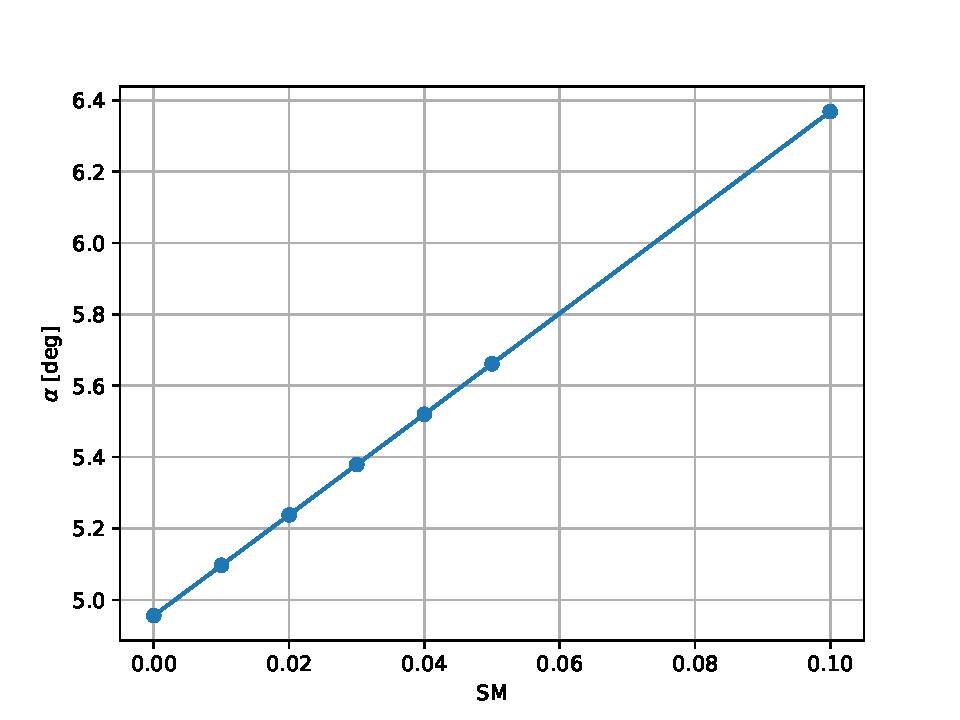
\includegraphics[keepaspectratio, width=\linewidth]{images/chap4/bwb_static_aoa}
		\caption{Angle of attack $\alpha$.}
		\label{fig:bwb_static_aoa_trim}
	\end{subfigure}
	\begin{subfigure}{0.5\textwidth}
		\centering
		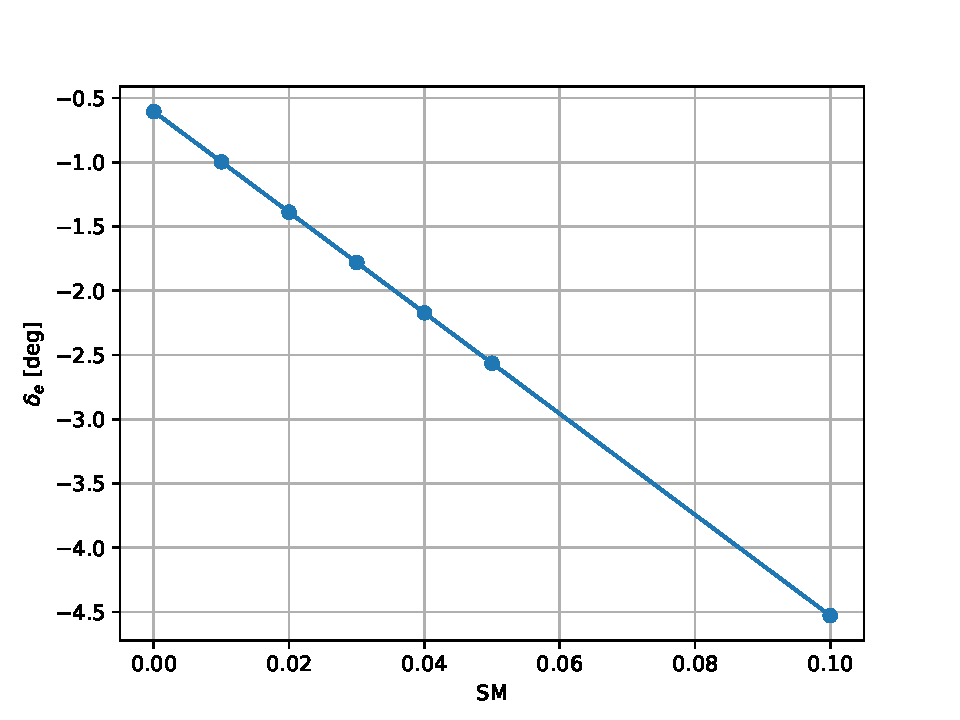
\includegraphics[keepaspectratio, width=\linewidth]{images/chap4/bwb_static_elev_angle}
		\caption{Elevon's deflection $\delta_{e}$.}
		\label{fig:bwb_static_elev_angle_trim}
	\end{subfigure}
	\begin{subfigure}{0.5\textwidth}
		\centering
		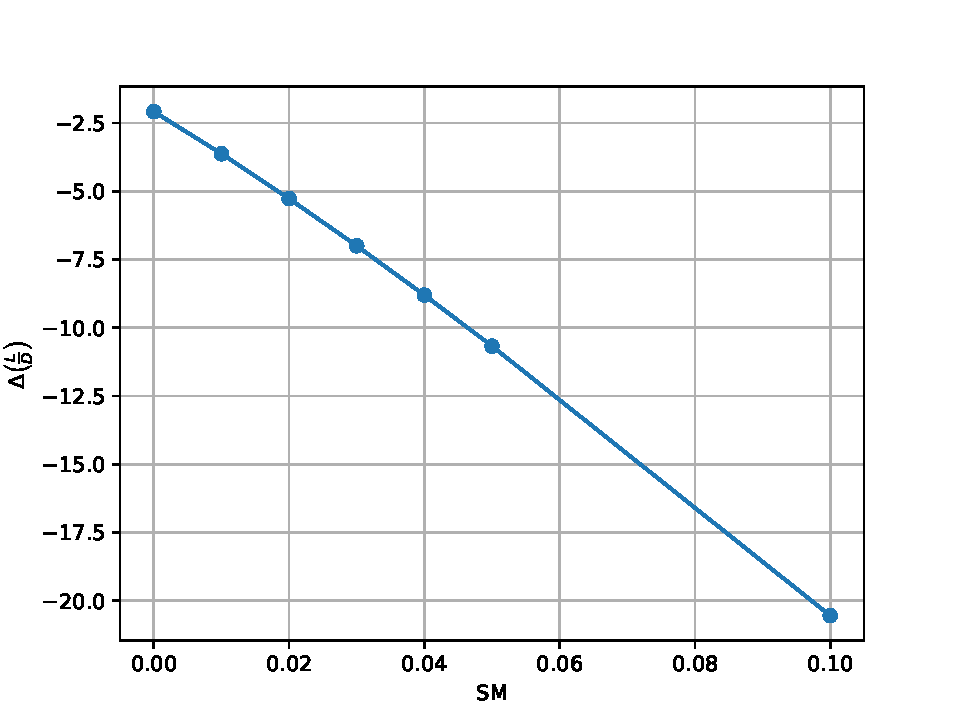
\includegraphics[keepaspectratio, width=\linewidth]{images/chap4/bwb_static_l2d_var}
		\caption{Variation of LoD value $\Delta\left(\frac{L}{D}\right)$.}
		\label{fig:bwb_static_l2d_var}
	\end{subfigure}
	\caption{Sensitivity analysis of trimmed condition with respect to the static margin. Quantities of interest considered are the angle of attack $\alpha$, the elevon's deflection $\delta_{e}$ and the variation of LoD value between trimmed and non trimmed condition $\Delta\left(\frac{L}{D}\right)$.}
	\label{fig:bwb_static_sensitivity_results}
\end{figure}
As expected, the SM strongly impacts the trim: for a margin of 10\% the difference in LoD between trim and no trim condition is about 20\%, as it decreases up to 2\% for a margin near to zero. 
This is due to the elevons deflection which is lower, and then reduces phenomenon of separation at trailing edge. 
It is also to note that the angle of attack, for a margin of 10\% is about 6~\si{\deg}, which is unfeasible for modern aircraft, meanwhile it reduces to 4.5~\si{\deg} for lower margin, that represents a more reasonable value. 

It is to highlight that in this case the center of gravity is fixed in order to obtain the desider SM, and this procedure is set only for stability studying purposes, but in real the SM represents an output and not an input of the system. 
As conclusion, for the BWB sizing reduced limits for the SM can be considered; to be conservative in the design and limit the risk, the case of unstable aircraft is not taken into account, and the modified condition states that the SM must be between 0 and 5\%, in place of 5 and 10\%:
\begin{equation}
	\label{eq:static_margin_bwb_limit}
	0 \leq \textrm{SM} \leq 0.05
\end{equation}

At this point, the longitudinal control has been studied; the final configuration chosen defines which is the space needed for control surfaces and the usable space for distributed propulsion or other systems. 
Next section will present the structural design, in order to get a surrogate model for the mass estimation.

\subsection{Blended Wing-Body structural design}
\label{subsec:chap4_bwb_structural_design}

\subsubsection{Modelling of the Blended Wing-Body internal structure}
\label{subsubsec:chap4_bwb_internal_structure_model}

For structural design it is intended the definition of the cabin concept and the design of structural elements, such as ribs, stringers and spars.
In Sec.~\ref{subsubsec:chap1_bwb_structure} three different cabin concepts have been analysed, pointing out their advantages and issues regarding some criteria, as specified in Table~\ref{tab:bwb_cabin_structure_synthesis}. 
In this research, it has been decided to consider an integrated cabin, because it represents the best compromise between passenger comfort, aerodynamics and structural loads. 

The structure is more complex than a conventional aircraft, since the cabin is not cylindrical anymore and elements pass through this part, so that the usable centerbody volume for payload is reduced.
Following the work done by Bradley~\cite{bib:bradley_bwb}, there are two spars, located at the leading edge (10\% of the chord) and at 70\% of the chord. 
In the integrated concept there is no separation between internal and external shell but just a single panels layer sustain both pressurization and aerodynamics load: these panels are modelled at thin plates with stringers to reinforce the structure, and they follow the thin plates theory~\cite{bib:megson}. 
Regarding the stringers, some literature references use the equivalent thickness philosophy to allow a fast and changeable stringer properies and configuration~\cite{bib:bradley_bwb, bib:mukhopadhayay_2005}. 
This is a possibility to reduce computational cost; however, for the present study, however, beam theory is applied~\cite{bib:megson} in order to have more accurate results. 
Finally, in the cabin there are some ribs to separate the centerbody from the transition zone, and eventually divide also the internal cabin.
A drawing of the final concept is shown in Fig.~\ref{fig:bwb_internal_structure_design}; ribs have been omitted for visualisation purposes. 
\begin{figure}[!h]
	\centering
	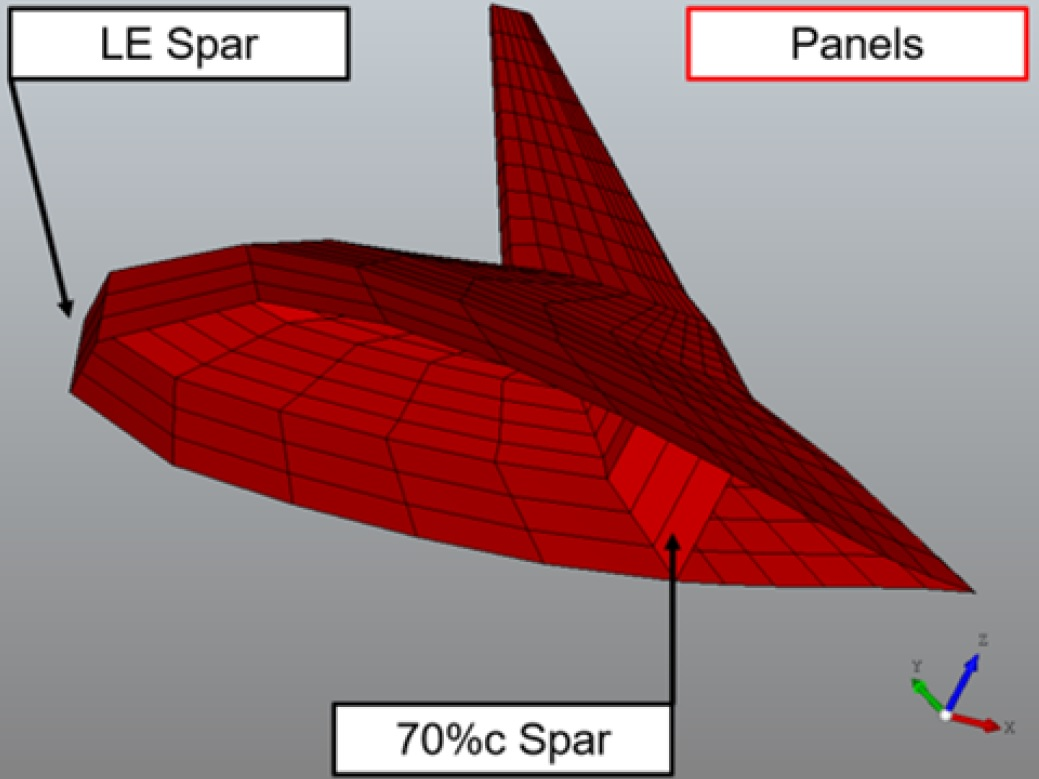
\includegraphics[keepaspectratio, width=0.4\textwidth]{images/chap4/bwb_internal_structure.jpg}
	\caption{BWB geometry visualisation; ribs have been omitted for clarity purposes.}
	\label{fig:bwb_internal_structure_design}
\end{figure}

The analysis is carried out through the FEM technique; tools used are the software Patran for modelisation and meshing~\cite{bib:patran} and Nastran for the structural analysis~\cite{bib:nastran}. 
Due to symmetry, only half of the BWB is considered, thus in the centerbody the symmetry boundary condition is applied.  

Concerning the material, the classical Aluminium Alloy 7075 (AA7075) used in aeronautics is considered by the time~\cite{bib:megson} and its properties are listed in Table~\ref{tab:aa7075_properties}.
\begin{table}[!h]
	\centering
	\begin{tabular}{l r l}
		\hline
		Young's modulus & 71.7 & \si{\giga\pascal} \\
		Poisson ratio & 0.33 & \\
		Max tensile strett & 138 & \si{\mega\pascal} \\
		Density & 2810 & \si{\kilogram\per\cubic\meter} \\
		\hline
	\end{tabular}
	\caption{Aluminium alloy 7075 properties~\cite{bib:megson}.}
	\label{tab:aa7075_properties}
\end{table}
It is to note that this choice is mainly dictated by the fact that this material is widely used in aeronautics, but it is in contrast with what is suggested in literature. 
Van Dommelen and Vos~\cite{bib:van_dommelen}, as well as Mukhopadhyay~\cite{bib:mukhopadhayay_2005} consider this material, but Liebeck argues that the high variation of pressure loads in the cabin favours the use of composite materials~\cite{bib:liebeck_1998}, and different authors consider deep sandwich composite with honeycomb aluminium core~\cite{bib:mukhopadhyay_2007}, isotropic and orthotropic composite materials~\cite{bib:mukhopadhyay_1996, bib:mukhopadhayay_2004}, and the advanced Carbon Fiber Reinforced Polymer (CFRP) material~\cite{bib:bradley_bwb}. 
In particular, this late one is used by Bradley to get the surrogate model described by Eq.~\eqref{eq:bwb_cabin_mass}.

\subsubsection{Static analysis}
\label{subsubsec:chap4_bwb_structure_static_analysis}

At the time, a static analysis is conducted to get the deformation and understand the feasibility of the concept to carry out the loads. 
Dynamic is not included, by this is not a limitation since such kind of analysis is more focused in studying the aeroelasticity effects, and this step can not be done if first it is ensured that in static condition the structure comply with sizing criteria. 
At the end, also an estimation of the mass can be done, which can be compared with the models adopted in FAST~\cite{bib:airbus_notes} and by Bradley~\cite{bib:bradley_bwb}.

The pressurization loads come from the Bradley reference again~\cite{bib:bradley_bwb}, which suggest a value of ultimate pressure differential of 18.6~\si{\psi}. 
Aerodynamics loads come from the CFD analysis previously done in Sec.~\ref{subsec:chap4_bwb_aero_cfd}: they are concerted into shear and bending applied to the outer rib of the centerbody. 
They are then multiplied by 1.5, which represents the ultimate design load for the sizing~\cite{bib:megson}. 

Results of this static analysis are shown in Fig.~\ref{fig:bwb_static_analysis_result} in terms of Von Mises stress; the optimisation of components to minimise the stress is carried out by the software. 
\begin{figure}[!h]
	\centering
	\begin{subfigure}{0.6\textwidth}
		\centering
		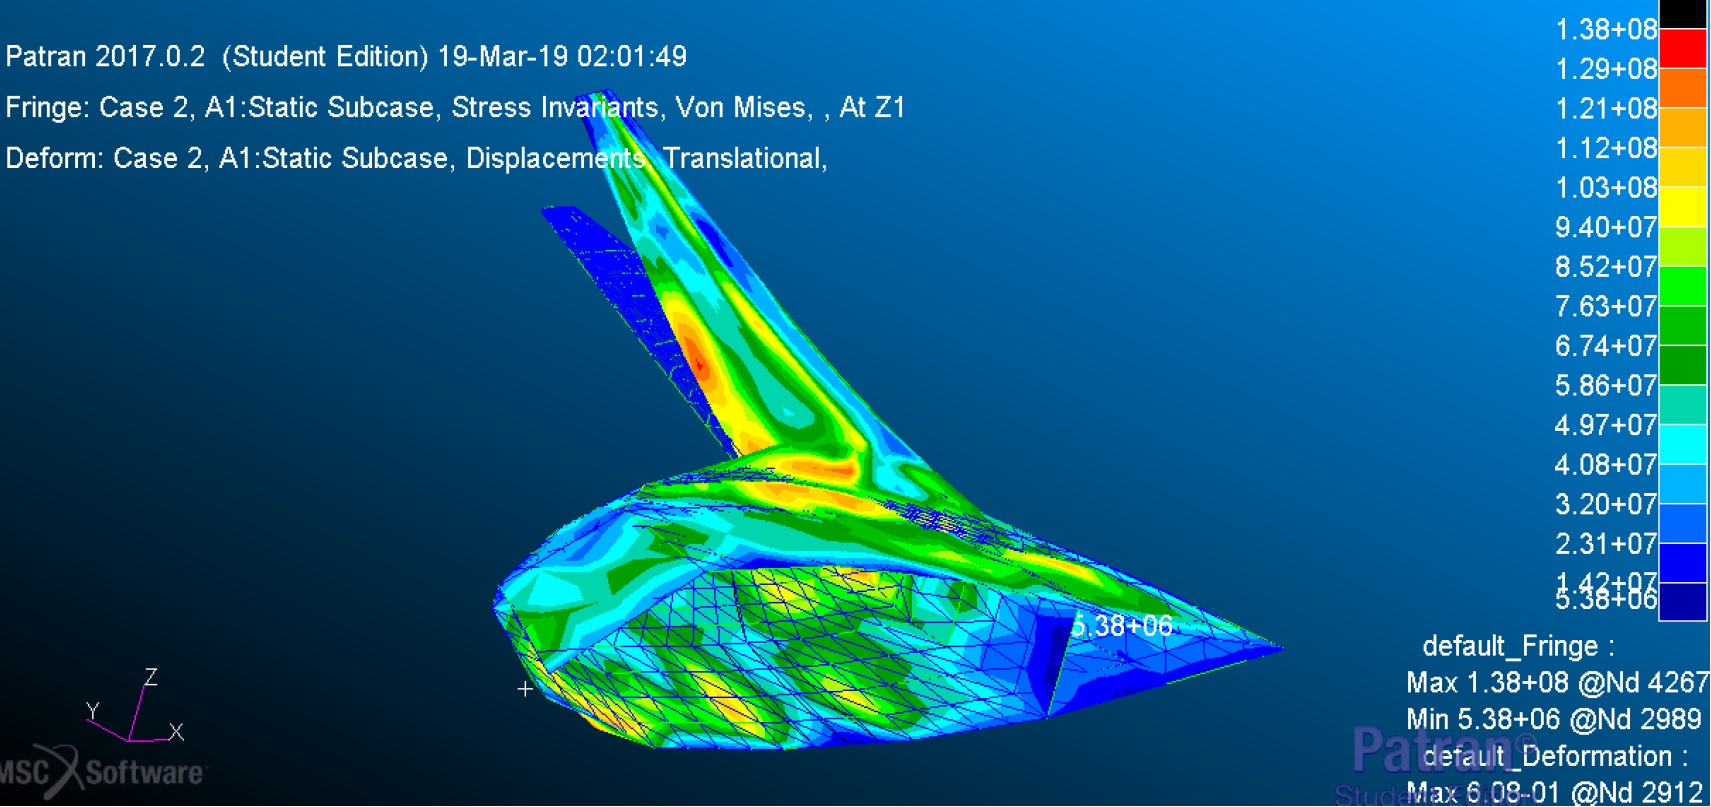
\includegraphics[keepaspectratio, width=\linewidth]{images/chap4/bwb_static_analysis_res_full_model.jpg}
		\caption{Full model.}
		\label{fig:bwb_static_analysis_full_model}
	\end{subfigure}
	\begin{subfigure}{0.6\textwidth}
		\centering
		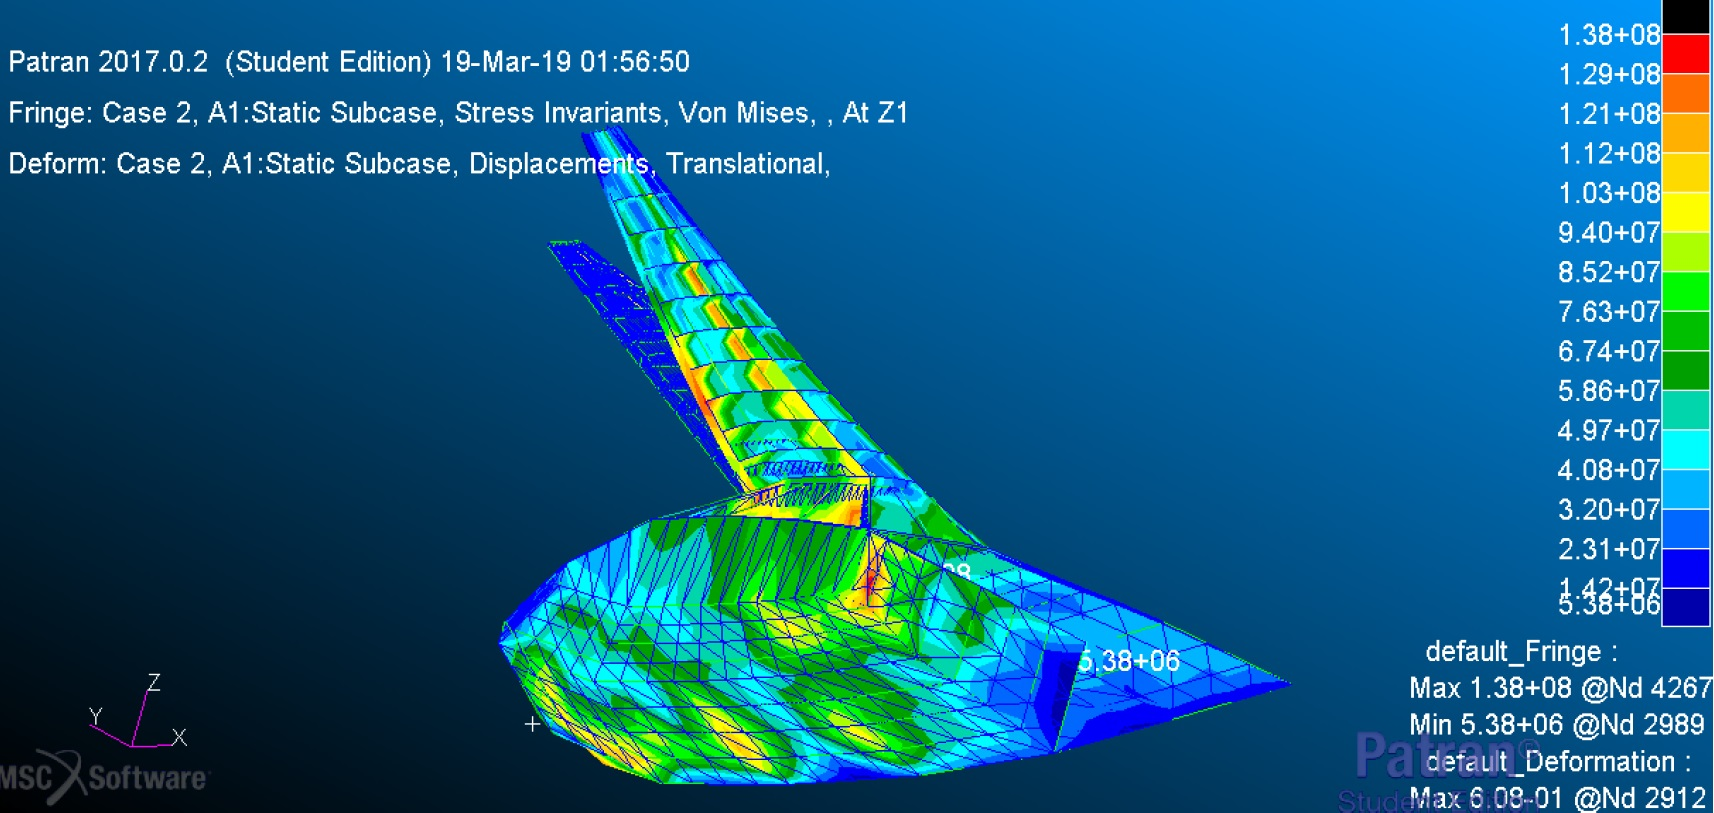
\includegraphics[keepaspectratio, width=\linewidth]{images/chap4/bwb_static_analysis_res_detail.jpg}
		\caption{Upper panels and Central ribs omitted for visualisation.}
		\label{fig:bwb_static_analysis_detail}
	\end{subfigure}
	\caption{Static analysis results for the BWB reference geometry design.}
	\label{fig:bwb_static_analysis_result}
\end{figure}
It can be observed that highest loads appear at the rear spar, in the pressurised area; in particular in the zone of connection between outer wing and centerbody. 
In this zone, the maximum Von Mises stress is of 136~\si{\mega\pascal}; due to the optimisation, this value is very close to the maximum allowable tensile stress. 
The wingtip is the most deflected zone, with a deflection of 6.1~\si{\centi\meter}.
Also wing torsion is detected, in the effect of a twist down more pronounced at the wingtip. 

The thicknesses of each component are reported in Table~\ref{tab:bwb_structure_thickness_results}.
Note that the ribs in the pressurised zone are three times thicker than that of the non-pressurised zone, because of the non-circular pressurization. 
\begin{table}[!h]
	\centering
	\begin{tabular}{l c}
		\hline
		\textbf{Component} & \textbf{Thickness~[\si{\meter}]} \\
		\hline
		Panels & 0.05 \\
		Ribs, non-pressurised & 0.0073 \\
		Ribs, pressurised & 0.033 \\
		Ribs, wing & 0.001 \\
		Spars & 0.0033 \\
		\hline
	\end{tabular}
	\caption{Structural components thickness for the static analysis of BWB reference geometry, case of maximum load factor $n=2.5$.}
	\label{tab:bwb_structure_thickness_results}
\end{table}
However, dimensions are limited and in agreement with what is obtained in conventional aircraft. 

From these data, it is possible to estimate also the total mass, which is of 31.4~\si{\tonne}: the centerbody accounts for 22.6~\si{\tonne}, meanwhile the outer wing accounts for 8.8~\si{\tonne}. 
In this calculation, the mass coming from the FEM has been multiplied by a factor 2, to account joints, fasteners and other components not taken into account in the FEM model~\cite{bib:mukhopadhyay_1996, bib:mukhopadhayay_2004}. 
The detailed mass breakdown for the components is illustrated in Fig.~\ref{fig:bwb_static_analysis_res_mb}.
The panels represent the majority of the mass, as it is responsible for sustaining both pressurization and aerodynamics load; also the stringers are slightly oversized since it incurs a bending due to the non-circularity of the centerbody. 
\begin{figure}[!h]
	\centering
	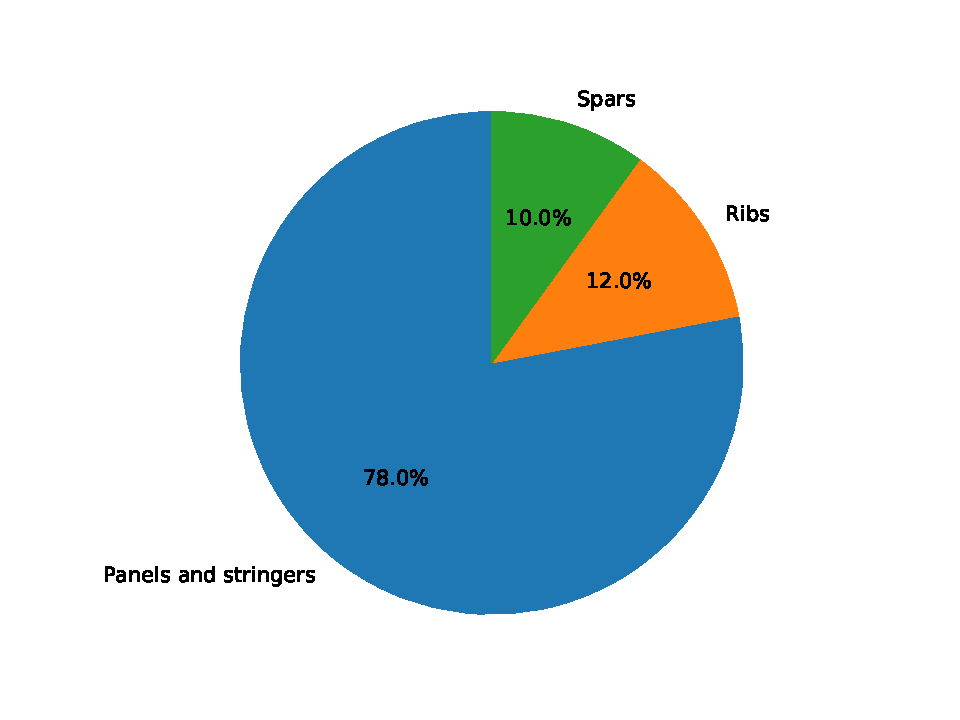
\includegraphics[keepaspectratio, width=0.6\textwidth]{images/chap4/bwb_internal_structure_breakdown}
	\caption{Structural components mass breakdown for the static analysis of BWB reference geometry.}
	\label{fig:bwb_static_analysis_res_mb}
\end{figure}

A comparison between some available data in literature (see Table~\ref{tab:bwb_struc_masses}) shows that the value of 31.4~\si{\tonne} is in the right order of magnitude for 250 or more passengers, but the value is doubled with respect to what has been estimated by Bradley for the 150 passengers BWB.
A more detailed comparison between the FEM analysis and the low fidelity models, that are surrogate models described in Eq.~\eqref{eq:bwb_cabin_mass} and the standard wing mass estimation used in FAST for the outer wing~\cite{bib:airbus_notes}, is reported in Table~\ref{tab:bwb_structure_method_comparison}.
Table~\ref{tab:bwb_structure_method_comparison} identifies the major source of error in the centerbody: indeed, the model used in FAST for outer wing specifies the AA7075 as material, and thus is quite accurate, meanwhile Bradley to get its surrogate model for the centerbody mass considers the CFRP material. 
\begin{table}[!h]
	\centering
	\begin{tabular}{l c c c}
		\hline
		& \textbf{FEM} & \textbf{Surrogate model} & \textbf{Difference} \\
		\hline
		Centerbody [\si{\tonne}] & 22.66 & 15.51 &  45.7\% \\
		Outer wing [\si{\tonne}] & 8.84 & 8.62 & 2.55\% \\
		\hline
	\end{tabular}
	\caption{Comparison between the FEM analysis and the surrogate model for centerbody and outer wing, for the BWB reference geometry case. Aluminium alloy 7075 is used as material.}
	\label{tab:bwb_structure_method_comparison}
\end{table}

The CFRM material has significantly different properties.
The density is 1550~\si{\kilogram\per\cubic\meter}, compared to 2810~\si{\kilogram\per\cubic\meter} for the AA7075, and the allowable tensile stress is 344~\si{\mega\pascal}, about 3 times higher than that of AA7075 (see Table~\ref{tab:aa7075_properties}). 

For validation purposes, a new analysis is carried out considering the CFRM as material for the centerbody; results for mass estimation are reported in Table~\ref{tab:bwb_bradley_model_validation}.
In this new case, the difference is less than 2\%, and then Eq.~\eqref{eq:bwb_cabin_mass} is validated.
\begin{table}[!h]
	\centering
	\begin{tabular}{l c c c}
		\hline
		& \textbf{FEM} & \textbf{Surrogate model} & \textbf{Difference} \\
		\hline
		Centerbody [\si{\tonne}] & 15.67 & 15.51 &  1.6\% \\
		\hline
	\end{tabular}
	\caption{Comparison between the FEM analysis and the surrogate model for centerbody and outer wing, for the BWB reference geometry case. CFRM material is used in the centerbody.}
	\label{tab:bwb_bradley_model_validation}
\end{table}

In conclusion, it has been shown that there is a good correlation between the FEM and the surrogate models, and thus the same model already adopted in FAST is retained for the outer wing, meanwhile for the centerbody Eq.~\eqref{eq:bwb_cabin_mass} is used, eventually with a corrective factor to consider the aluminium alloy in place of the CFRM as material. 

At this point, it is time to pass to the nacelle integration, in order to estimate the effect of an ingesting boundary layer. 
This will be the goal of the next section. 

\subsection{Nacelle integration in the Blended Wing-Body architecture}
\label{subsec:chap4_nacelle_integration}

This section studies the integration of the nacelle in a BWB architecture, in order to estimate the effect of an ingesting device as the BLI. 
At this stage of the research, so much resources have been deployed in the CFD analysis that it has not been possible to carry out this analysis using the CFD, due to the high number of hours required by the modelisation, meshing and analysis. 

For this reason, the study is carried out using the software MSES, developed at MIT by Mark Drela~\cite{bib:mses}. 
The code is a medium fidelity software, that relies on hybrid methods between potential flow and CFD regression analysis, capable to analyse the flow field for multibody objects. 
Also, one of its greatest features is the possibility to optimise the body thanks to the LINDOP, a subroutine of MSES~\cite{bib:lindop}. 
LINDOP has been developed mainly for the optimisation of multi-element airfoils~\cite{bib:drela_1993}, which is interesting to optimise a nacelle integrated in a BWB.
The main limitation of MSES is that it is a 2D software, and all the three-dimensionality effects, which are not trivial in case of ingesting propulsors, are neglected.
 
The BWB reference geometry, shown in Fig.~\ref{fig:bwb_ref_geometry}, is divided into different slices, and each one is studied separately using MSES. 
At the end, the global $C_L$ and $C_D$ values are obtained through numerical integration~\cite{bib:rodriguez_1999}.
The engines are distributed only in the centerbody part, for what has been said in Sec.~\ref{subsec:chap4_bwb_control}; the integrated geometry is shown in Fig.~\ref{fig:bwb_nacelle_geom}, in the symmetry plane (that of maximum length).
\begin{figure}[!h]
	\centering
	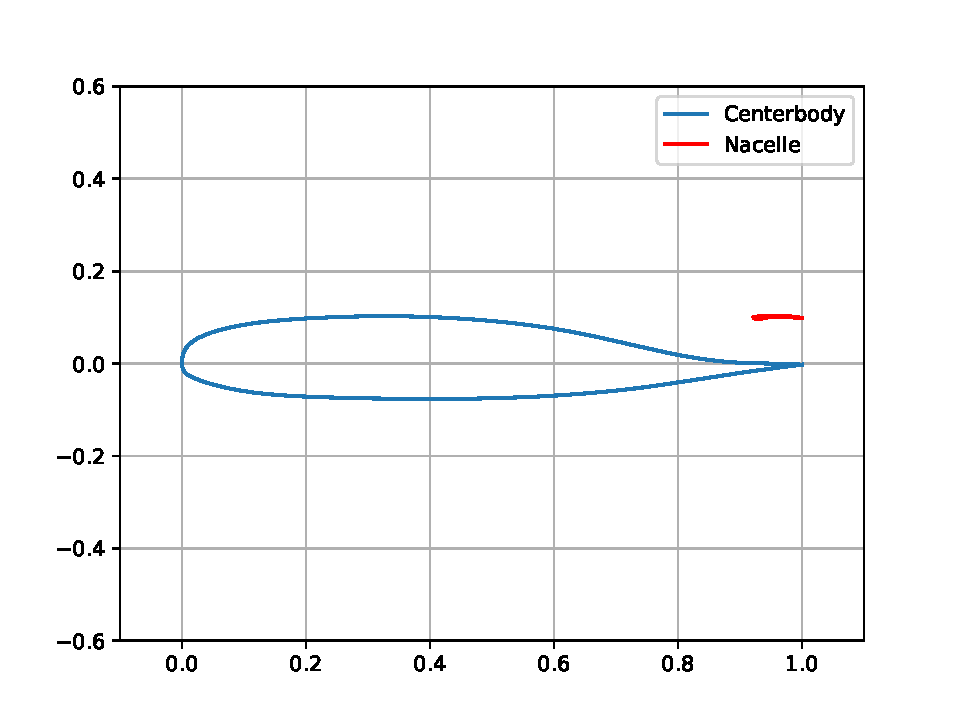
\includegraphics[keepaspectratio, width=0.6\textwidth]{images/chap4/bwb_nacelle_geom}
	\caption{BWB reference geometry, together with integrated nacelle, at the symmetry section.}
	\label{fig:bwb_nacelle_geom}
\end{figure}

The flow condition for the analysis corresponds to the estimated design point and they are reported in Table~\ref{tab:mses_flow_condition}.
\begin{table}[!h]
	\centering
	\begin{tabular}{l c}
		\hline
		Mach number & 0.78 \\
		Angle of attack & 1.5~\si{\deg} \\
		Reynolds & $6.24\times10^6$ \\
		$C_T$ & $1.66\times10^{-3}$ \\
		\hline
	\end{tabular}
	\caption{Condition for the study of nacelle effect in MSES.}
	\label{tab:mses_flow_condition}
\end{table}
The value of thrust coefficient is estimated by the knowledge of the mass; in balanced flight it is possible to write
\begin{equation}
	\label{eq:thrust_balanced_flight}
	T = \frac{m_{cr}g}{\left(\frac{L}{D}\right)_{\max}}
\end{equation}
The value of LoD comes from the CFD analysis. 
A total of 32 engines is used: this is the maximum number of engines that can be placed in the zone of interest.
This value is estimated from the ducted fan sizing procedure described in Sec.~\ref{subsec:chap3_duct_fan_sizing}.

The initial geometry for the nacelle is the NACA64A010; using the code LINDOP it is then optimised in order to reduce the drag coefficient, section by section. 
Drela suggests to use a multipoint optimisation~\cite{bib:drela_1993}: in fact, with the single point there are very good performance at the optimisation point, but in off design conditions they may not be satisfactory. 

The objective function is
\begin{equation}
	\label{eq:mses_multipoint_obj}
	f = 0.75 C_{D_{M=0.6}} + C_{D_{M=0.7}} + 1.25 C_{D_{M=0.78}}
\end{equation}
where the subscripts indicate the Mach number to which the $C_D$ refers. 
In this way, all the transonic regime is covered, and the design point has more weight in the optimisation than the others. 

The final nacelle geometry, after the optimisation, is shown in Fig.~\ref{fig:bwb_nacelle_geom_detail}, meanwhile the performance of the geometry with nacelle integrated is reported in Fig.~\ref{fig:clcd_nacelle_integration_performance}, varying the Mach number. 
On the left there is the non optimised case, meanwhile on the right the optimised one.
\begin{figure}[!h]
	\centering
	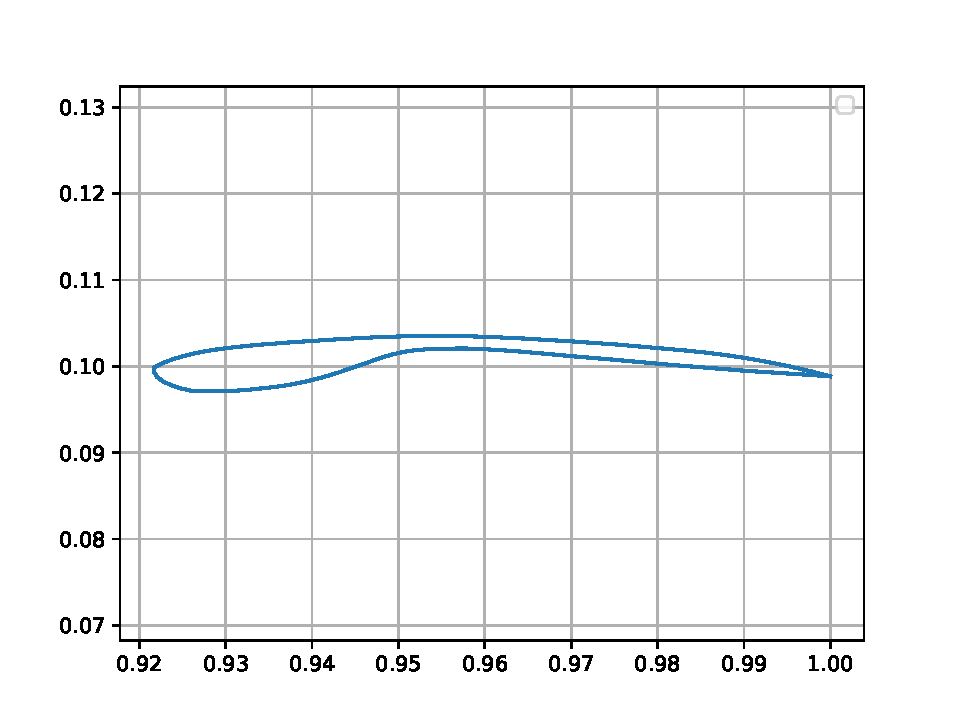
\includegraphics[keepaspectratio, width=0.6\textwidth]{images/chap4/bwb_nacelle_geom_detail}
	\caption{Detail of the optimised nacelle, mounted on the BWB.}
	\label{fig:bwb_nacelle_geom_detail}
\end{figure}
\begin{figure}[!h]
	\centering
	\begin{subfigure}{0.45\textwidth}
		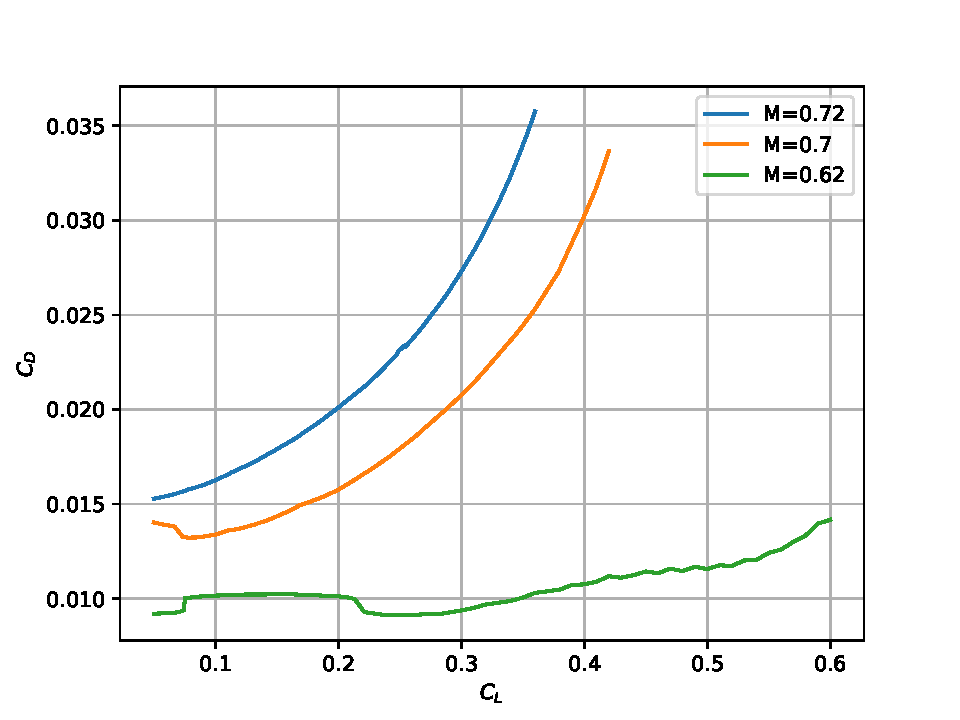
\includegraphics[keepaspectratio, width=\linewidth]{images/chap4/clcd_nacelle_non_opt_comparison}
		\caption{Non optimised case.}
		\label{fig:clcd_nacelle_non_optim}
	\end{subfigure}
	\begin{subfigure}{0.45\textwidth}
		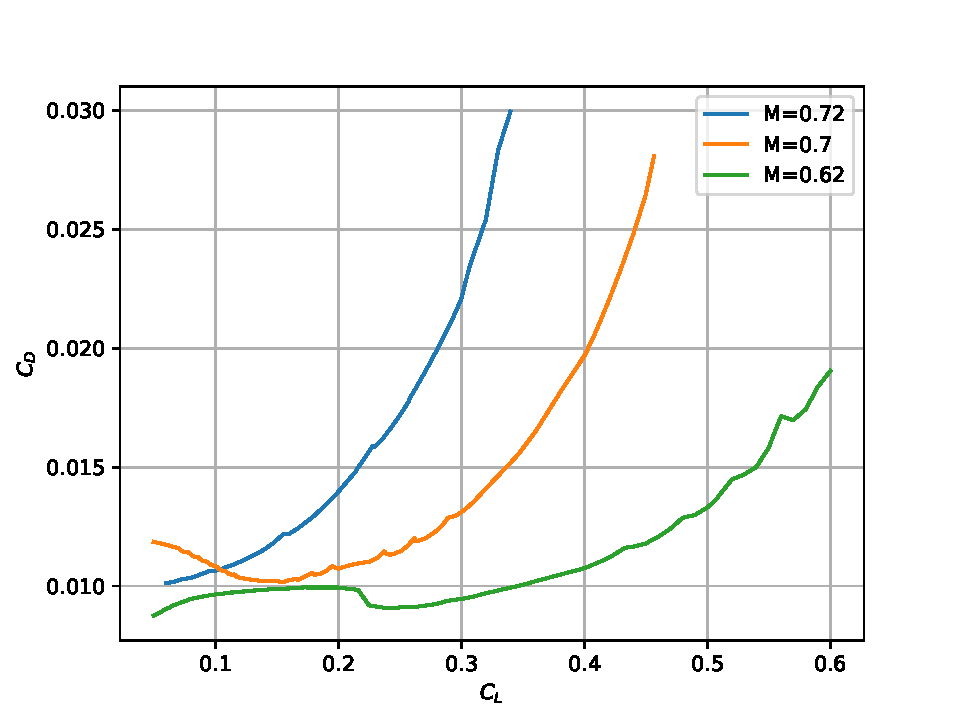
\includegraphics[keepaspectratio, width=\linewidth]{images/chap4/clcd_nacelle_opt_comparison}
		\caption{Optimised case.}
		\label{fig:clcd_nacelle_optim}
	\end{subfigure}
	\caption{Performance comparison between the non optimised and optimised nacelle geometry using MSES.}
	\label{fig:clcd_nacelle_integration_performance}
\end{figure}

From the comparison of Fig.~\ref{fig:clcd_nacelle_integration_performance} emerges that the baseline has not very good performances, despite the initial geometry of NACA 641010 is designed for transonic purposes~\cite{bib:anderson_aero}, but after the optimisation the wave drag is well reduced, and thanks to the multipoint adopted in Eq.~\eqref{eq:mses_multipoint_obj} the reduction occurs for all the Mach numbers.

To estimate the effect of a BLI device, the procedure suggested by NASA is used~\cite{bib:bwb_n3_vol2}. 
The drag coefficient can be decomposed in two terms, one related to the dissipation of energy $C_{\phi}$ and another one to the vortex dissipation $C_{E_{v}}$:
\begin{equation}
	\label{eq:cd_energy_decomposition}
	C_D = C_{\phi} + C_{E_{v}}
\end{equation}

In case of ingestion, the term related to the energy dissipation is modified as
\begin{equation}
	C_{\phi}^{'} = C_{D_{p}} - f_{BLI} \frac{K_{\infty}-K_{TE}}{\rho_{\infty}V_{\infty}^3S_w}
\end{equation}
where $C_{D_{p}}$ is the parasite drag of non ingesting case, $f_{BLI}$ the fraction of the body's kinetic energy defected ingested by the engine, $K_{\infty}$ and $K_{TE}$ the kinetic energy at inflow and trailing edge respectively. 

From MSES it is possible to obtain all the boundary layer parameters, in particular the dispacement and kinetic energy thickness: a comparison between the non ingesting and ingesting case is shown in Fig.~\ref{fig:bwb_nacelle_bl_param_comp}.
\begin{figure}[!h]
	\centering
	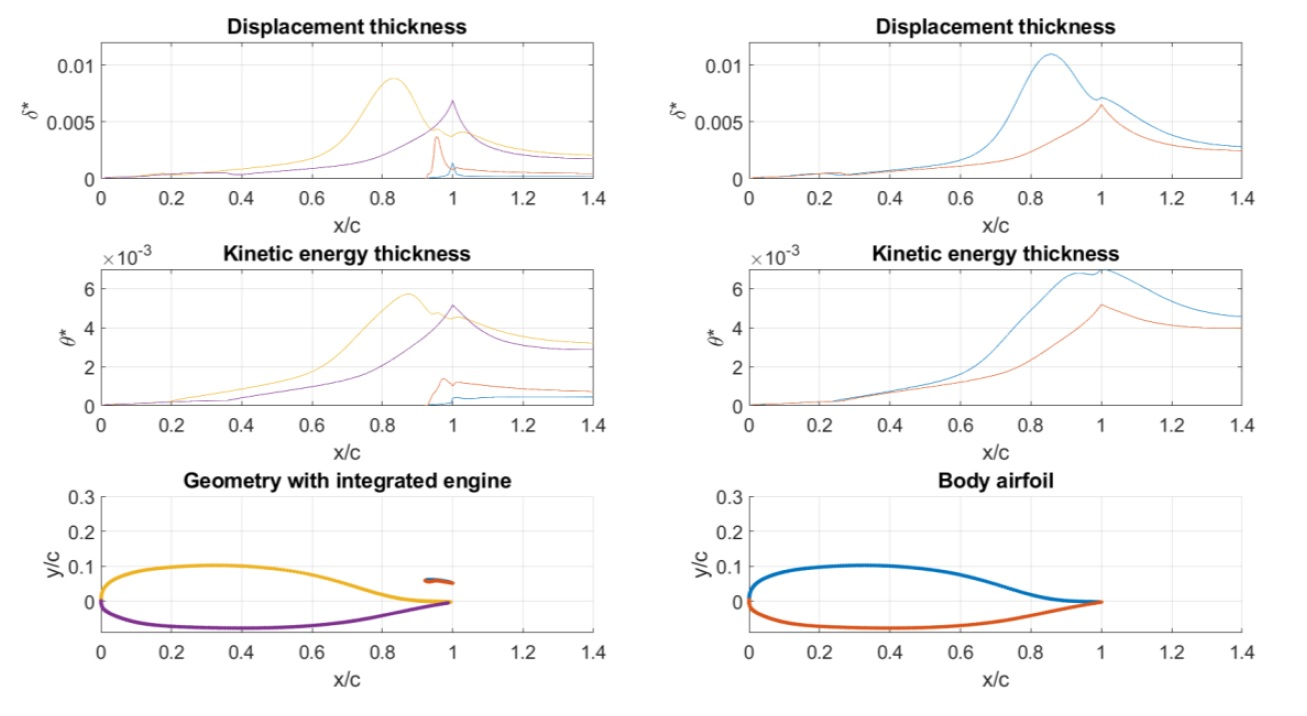
\includegraphics[keepaspectratio, width=\textwidth]{images/chap4/bwb_nacelle_bl_param.jpg}
	\caption{Displacement thickness and kinetic energy thickness comparison between the integrated geometry and the isolated body geometry.}
	\label{fig:bwb_nacelle_bl_param_comp}
\end{figure}

Thanks to the knowledge of these parameters, through integration it is possible to estimate $f_{BLI}$ and $C_{\phi}$. 
For the condition of Table~\ref{tab:mses_flow_condition}, the BLI effect is estimated in a reduction on the drag coefficient of 14\%. 
The value is in agreement with estimations given by IATA reports~\cite{bib:iata_annex}, despite the limitations due to the 2D assumption. 

In real, for an ingesting device a flow distorsion appears, as explained in Sec.~\ref{subsubsec:chap1_bli_review}, which worsen the benefits; on the other hand, an ingesting architecture saves fuel because the nacelle wetted area is reduced, which is beneficial for aerodynamics and mass. 
So at the end the benefits coming from the BLI are a balance between these effects. 
A more accurate estimation can be obtained only using the CFD; for the purposes of this research these benefits are simply modelled with a corrective factor. 
To be conservative, a reduction in $C_D$ of 10\%, in place of 14\% is considered for the evaluation of the concept. 
This value is in agreement with other studies on the BLI effects~\cite{bib:iata_annex, bib:steiner_2012, bib:uranga}.

The estimation of BLI is the last step that had to be carried out to finally correct the models; next section is deputed to define the parametrization for the BWB planform sizing and the internal arrangement. 

\subsection{Blended Wing-Body design synthesis}
\label{subsec:chap4_bwb_arrangement}

This section provides an exhaustive analysis of the decisions done in the BWB sizing: at first the parametrization adopted is presented, and then the final concept, including the subsystem positioning, is described.
It is to highlight that most of the assumptions done in the second part are on a level of detail that can not be included in the conceptual sizing loop; however decisions on cargo, exit doors and so on must be done in order to give feasibility to concept, and limit the usable volume in the sizing process. 

\subsubsection{Planform sizing}
\label{subsubsec:chap4_bwb_centerbody_sizing}

Since the BWB relies on the idea of having a whole lifting surface, it is schematised as a wing with three or more sections, and the parametrization here adopted follows this concept. 
The planform is divided into three parts: centerbody, transition zone and outer wing, each one considered as a wing section. 
The entries for the sections are the same of a wing planform: sweep angle, taper ratio, span or aspect ratio, and thickness to chord ratio. 

The parametrization is shown in Fig.~\ref{fig:bwb_planform_scheme}, with the main parameters noted on the image. 
\begin{figure}[!h]
	\centering
	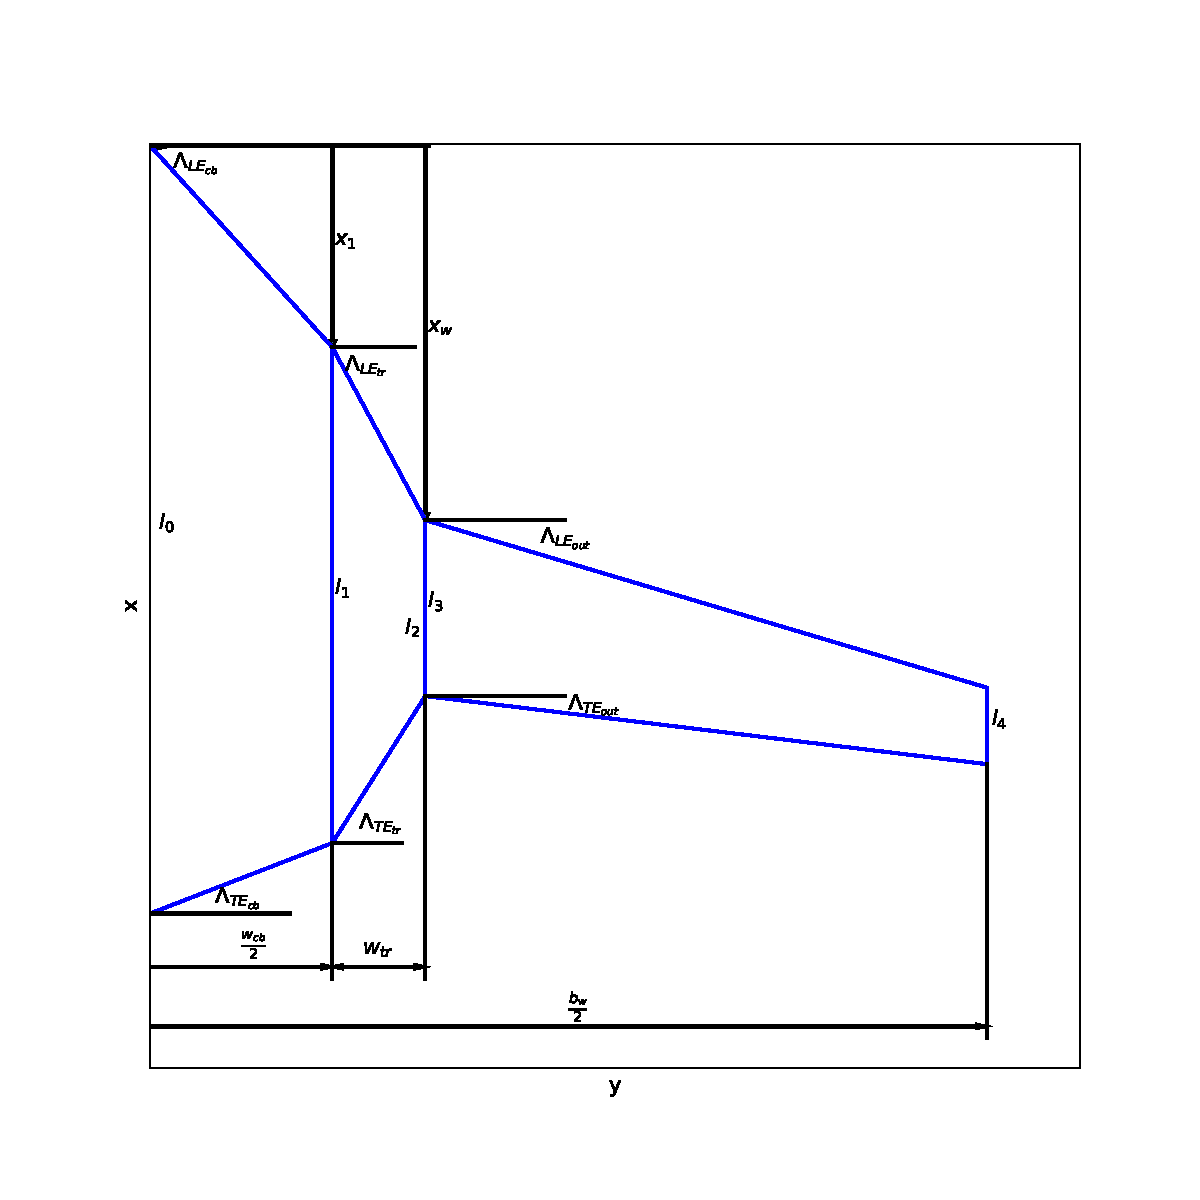
\includegraphics[keepaspectratio, width=0.8\textwidth]{images/chap4/bwb_planform_scheme}
	\caption{Planform scheme for the Blended Wing-Body sizing.}
	\label{fig:bwb_planform_scheme}
\end{figure}
The hardest section to model is the central one, since it has to supply enough space for seats allocation; once that the cabin is fully sized, transition zone and outer wing can be easily obtained. 
The explanation of the sizing starts indeed from the cabin.

\subsubsection{Cabin modelling}
\label{subsubsec:chap4_bwb_cabin_model}

The cabin must allow enough space for the passengers allocation; following the work of Bradley~\cite{bib:bradley_bwb} the cabin is divided into bays, separated by ribs in an integrated design. 
Each bay is single aisle, with two lines of seats. 

The starting point for the sizing procedure is the definition of an equivalent tube-and-wing configuration, with the same number of passengers per row of a bay, to know the length required for all the seats:
\begin{equation}
\label{eq:taw_eq_length}
L_{req}=\sum_{i=1}^{3}N_{r_{i}}L_{i} + N_{exit}W_{exit}
\end{equation}
where $N_{r_{i}}$ is the number of rows and $L_i$ the length of the seats for the $i$ class, $N_{exit}$ and $W_{exit}$ the number and the width of exit doors. 
In the case of a single class, which is the case of interest for the type of aircraft selected, $N_r=\frac{N}{6}$, where $N$ is the number of passengers and 6 represents the seats per row in economic class.

The number of bays is then computed considering a rectangular cabin:
\begin{equation}
\label{eq:bays_number}
N_b=\left[\frac{L_{req}}{l_{out_{\max}}}\right]+1
\end{equation}
where $l_{out_{\max}}$ is the maximum allowable outermost wall length, computed as it will be explained later, and the square brackets represent the integer function.

With some geometrical considerations, it is possible to write an equation to get the total length available for seats in the BWB (see Fig.~\ref{fig:bradley_seats_arrangement} for clarity):
\begin{equation}
\label{eq:bwb_total_length}
L_{tot} = \sum_{i=1}^{N_b}\left[l_{out} + \frac{1}{2}\left(i-1\right)w_b\tan\Lambda_{cb}\right] = N_bl_{out} + \frac{1}{2}w_b\tan\Lambda_{cb}\sum_{i=1}^{N_b}\left(i-1\right)
\end{equation}
with $l_{out}$ outermost wall length, $w_b$ the bay of a single width and $\Lambda_{cb}$ the centerbody sweep angle, computed at leading edge. 
\begin{figure}[!h]
	\centering
	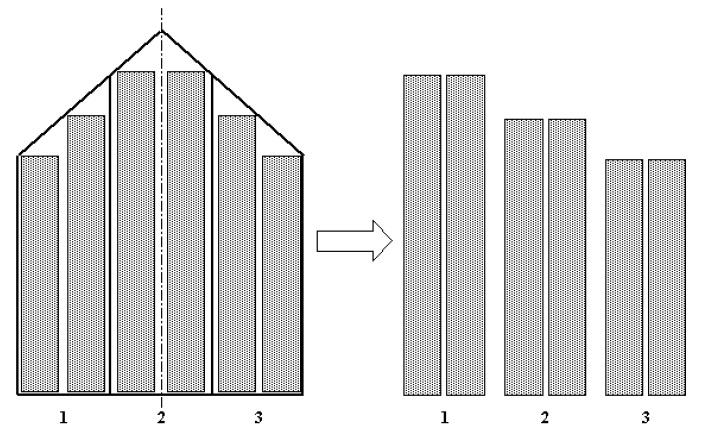
\includegraphics[width=0.6\textwidth, keepaspectratio]{images/chap4/bwb_bradley_equivalent_bay.jpg}
	\caption{Seats arrangements for a three class BWB configurations.}
	\label{fig:bradley_seats_arrangement}		
\end{figure}

Setting $L_{req}=L_{tot}$ yields to the following expression to compute the actual outermost wall length:
\begin{equation}
\label{eq:outermost_wall_length}
l_1 = \frac{L_{tot}-\frac{1}{2}w_b\tan\Lambda_{LE_{cb}}\sum_{i=1}^{N_b}\left(i-1\right)}{N_b}
\end{equation}
and the cabin results fully defined, since the centerbody is then obtained as follows:
\begin{equation}
\label{eq:center_section_length}
l_0 = l_1 + \frac{N_b}{2}w_b\tan\Lambda_{LE_{cb}}
\end{equation}
A margin is then taken to allocate horizontal aisle and toilets, according to preliminary methods from Roskam~\cite{bib:roskam_partIII}. 
These dimensions are only related to the pressurised cabin; recalling that this occupies the 70\% of the centerbody, the total length is obtained dividing these values by 0.7.

This procedure allows to size a cabin, but it depends on the value of $l_{out_{\max}}$, which is unknown at the beginning. 
Bradley suggests to use 15.6~\si{\meter}, with a centerbody sweep angle of 45~\si{\deg}. 
In the reference paper, unfortunately, there are no information about the origin of this value~\cite{bib:bradley_bwb}; in this research it has been considered that the maximum length is deduced from the centerbody taper ratio. 
Since the value $l_0$ is unknown, an iterative procedure is needed. 

The length must also supply the cabin vertical arrangement criterion. 
According to Airbus, the minimum cabin height has to be 1.95~\si{\meter}; considering a 12\% structural margin~\cite{bib:raymer, bib:roskam_partIII} yields to a total height of 2.18~\si{\meter}.
From the value of thickness-to-chord ratio it is then possible to estimate the total length needed in this section to provide such height:
\begin{equation}
\label{eq:outermost_section_length}
l_1 = \frac{h_{min}}{\left(\frac{t}{c}\right)_{cb}}
\end{equation}
An iterative procedure is set up to find the values of thickness-to-chord ratio and maximum outmost length of the final geometry. 

In this way, the cabin planform is finally sized, but nothing has been said on the airfoil sizing yet. 
The only information known is that reflex airfoils are needed for stability purposes, as recalled several times~\cite{bib:alex, bib:nickel}.
The most correct way is to include the airfoil sizing within the optimisation procedure, but this is unfeasible without the application of CFD, which is very costly. 

The relation described by Eq.~\eqref{eq:outermost_section_length} can help to choose a value of thickness-to-chord ratio able to ensure enough space at the section with maximum thickness, but this is not sufficient to ensure that all the cabin fits in the profile.
In fact, the minimum height criterion must be valid in all the sections, and the most stringent one is that corresponding to the last row of passengers (70\% of the chord).

The relative thickness can be changed in post processing where the planform is obtained, but this is not coherent with the sizing process, and all the results will be misleading. 
Thus it is a key point to have the possibility to get as output a thickness-to-chord ratio that allows to choice an airfoil without the fitting problems. 
To do that, the analytic thickness distribution must be known, to be able to constraint the height value at 70\% of the cabin. 

The thickness distribution is know only for the NACA family~\cite{bib:abbott}, where 
\begin{equation}
\label{eq:thickness_distribution}
\pm y_t = \frac{t}{0.20}\left(0.2969\sqrt{x}-0.1260x-0.3516x^2+0.2843x^3-0.1015x^4\right)
\end{equation}
with $y_t$ the thickness distribution, $t$ the maximum thickness and $x$ the abscissa; all of these parameters are in percentage of the chord. 

Requiring that $y_t c=\frac{1.95\times 1.12}{2}$ at $x=0.7$ it is possible to correct the initial estimation of thickness-to-chord ratio, that suites the cabin height requirements. 
Once that this value is obtained within the sizing loop, it is possible to choose one of the NACA airfoil with the chosen relative thickness, avoiding the problem of fitting.
In particular, the 5-digit series is worthy of attention because it is a family of reflex airfoil, that provides almost zero momentum coefficient.  

The condition described by Eq.~\eqref{eq:thickness_distribution} must be written for all the sections: in fact, the most stringent is the outmost section, where the length is smaller, but applying a constant thickness-to-chord ratio results in an oversizing of other sections, worsening the aerodynamics. 
For simplicity, in the sizing procedure only the symmetry and the outermost section are considered, and the mean value of thickness-to-chord ratio is taken for aerodynamics calculation. 

However, it has to be remarked that the choice of NACA family has been done for simplicity and to close the problem, but it is just a first assumption that needs to be redefined in a more detailed design, with the help of high fidelity optimisation.

\subsubsection{Transition zone and outer wing modelling}
\label{subsubsec:chap4_tr_zone_outer_wing_model}

Once that the centerbody dimensions are got, the others come as consequence. 
For continuity, the root chord of the transition zone is equal to the tip chord of the centerbody; the tip chord of this zone is obtained by the definition of taper ratio as
\begin{equation}
	\label{eq:transition_tip_chord}
	l_2 = l_1 \lambda_{tr}
\end{equation}

The surface of transition zone results to be:
\begin{equation}
	\label{eq:transition_surface}
	S_{tr} = \frac{\left(l_2 + l_1\right)w_{tr}}{2} = \frac{\left(1+\lambda_{tr}\right)l_1 w_{tr}}{2}
\end{equation}
where $w_{tr}$ is the width of transition zone, set to satisfy allocation criterion that will be later explained.

The sweep angle for this zone is not an input of the parametrization, but it is an output, according to the wing position:
\begin{equation}
	\label{eq:transition_sweep}
	\Lambda_{tr} = \arctan{\frac{x_w - x_1}{w_{tr}}} = \arctan{\frac{x_w - w_{cb}\tan{\Lambda_{LE_{cb}}}}{w_{tr}}}
\end{equation}

The total planform surface is set by a top level criterion, as will be explained in next section.
The knowledge of this surface plus the centerbody and the transition surface yields to the surface of outer wing solely:
\begin{equation}
	\label{eq:outer_wing_surface}
	S_{w_{out}} = S_w - S_{cb} - S_{tr}
\end{equation}
and from Eq.~\eqref{eq:transition_surface} written for outer wing the root chord $l_3$ is obtained:
\begin{equation}
	\label{eq:l3_out_wing}
	l_3 = \frac{2 S_{w_{out}}b_{out}}{1 + \lambda_{w_{out}}}
\end{equation}
with $b_{out}=b_w - w_{tr} - w_{cb}$. 
Of course, the total span is obtained by the aspect ratio definition as 
\begin{equation}
	\label{eq:total_span}
	b_w = \sqrt{AR_w S_w}
\end{equation}

In this way, all the planform dimensions are fully defined. 
On the other plane, the thickness-to-chord ratio is sized considering space needing for the transition zone, and aerodynamics considerations, as for conventional aircraft, for the outer wing. 

For sake of clarity, Table~\ref{tab:bwb_geom_input_sum_up} reports all the geometrical entries needed for the adopted parametrization. 
\begin{table}[!h]
	\centering
	\begin{tabular}{c c c c}
		\hline
		\textbf{Global} & \textbf{Centerbody} & \textbf{Transition zone} & \textbf{Outer wing} \\
		\hline
		Aspect ratio & Sweep angle & Taper ratio & Sweep angle \\
		Total area & Minimum cabin height & & Relative thickness \\
		& Taper ratio & & Position \\
		& Number of passengers & & Taper ratio \\
		\hline 
	\end{tabular}
	\caption{Sum up of geometrical entries for the BWB parametrization.}
	\label{tab:bwb_geom_input_sum_up}
\end{table}

Finally, at this point the overall illustration, including some assumptions on the subsystems position, can be drawn, as in next section.

\subsubsection{Subsystem positioning}
\label{subsubsec:chap4_bwb_subsystem_position}

The rendering of the Blended Wing-Body with distributed electric propulsion, final goal of this research, is shown in Fig.~\ref{fig:bwb_dep_render}, as in OpenVSP. 
The engines are distributed at the trailing edge, in the centerbody, leaving free all the outer wing surface for control surfaces, as described in Sec.~\ref{subsec:chap4_bwb_control}. 
At the wing tip there are two winglets, used also as vertical tails for lateral control. 
\begin{figure}[!h]
	\centering
	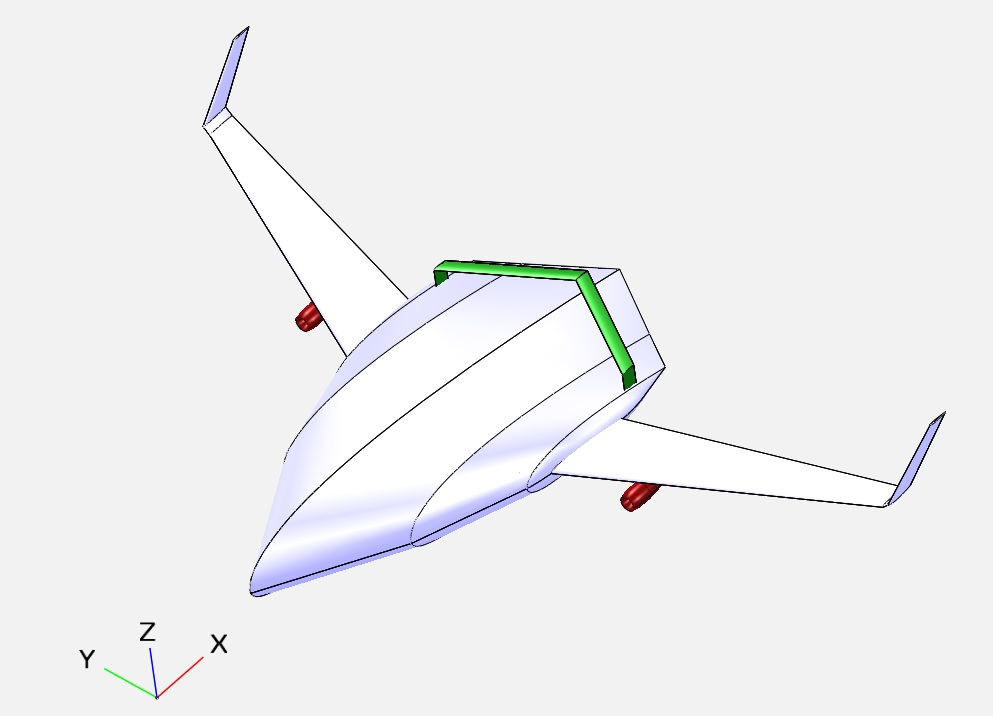
\includegraphics[keepaspectratio, width=0.6\textwidth]{images/chap4/bwb_dep_render.jpg}
	\caption{Final rendering of Blended Wing-Body with distributed propulsion.}
	\label{fig:bwb_dep_render}
\end{figure}

It is to clarify that Fig.~\ref{fig:bwb_dep_render} just illustrates how the final concept looks like, but it is not yet a result of a proper sizing. 

The first issue to deal with regards the boarding door, which is a point not well treaten in literature. 
Some of the proposed concepts show boarding doors only at the leading edge (see \textit{i.e.} \cite{bib:dzyne_bwb, bib:bwb_n3_vol1}), but such a position may create problems since it does not account for the CS specification for large aeroplanes~\cite{bib:cs_evacuation}. 
The document states that each side of the aircraft should be equipped with two doors of type I~\cite{bib:roskam_partIII} for boarding, and two doors of type III for evacuation~\cite{bib:roskam_partIII}. 
The first category is the most critical since they require fixed dimensions and a positioning at the front and the rear of the aircraft, menawhile the second category does not have any constraint on dimensions, but they just satisfy a minimum distance between them. 

The requirement of boarding doors at the front and the rear of the aircraft has also been noted by Airbus, both for certification and acceptance purposes. 
A suitable arrangement for seats and boarding doors is shown in Fig.~\ref{fig:bwb_boarding_door_position}; the coloring helps to understand how each passenger is close to a door or not. 
\begin{figure}[!h]
	\centering
	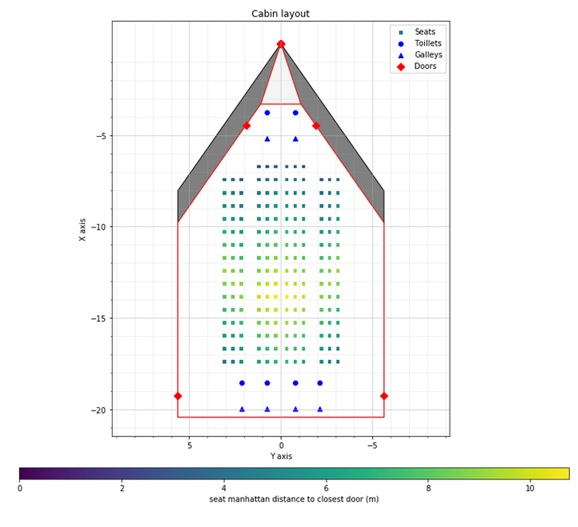
\includegraphics[keepaspectratio, width=0.6\textwidth]{images/chap4/bwb_boarding_door_position.jpg}
	\caption{Seats arrangement and boarding doors position assumption for the BWB geometry.}
	\label{fig:bwb_boarding_door_position}
\end{figure}
In Fig.~\ref{fig:bwb_boarding_door_position} emergency exits are not noted, but they are assumed to be in the central part of the cabin, coming out on the outer wing, as in a conventional aircraft. 
This configuration has been validated by Airbus expertes, however it is to remark that it is just a proposition and not a detailed study. 
All related issues, such as the corridor that passes through the structure to allow passengers entrance, and the impact of the necessary cut-off on the structure must be detailed in future development. 
Note also that such configuration constraints the outer wing trailing edge, in order to leave enough space for the rear door. 

One of the potential advantages is that the required boarding time may be reduced, thanks to the wider cabin that allows passengers to move in the cabin more freely. 
The colouring of Fig.~\ref{fig:bwb_boarding_door_position} shows that there are just few places that are farer from an exit, but in mean all the others are close enough to reach its place in a reasonable time. 

To confirm this theory, a boarding simulation is carried out, using a software called PAXelerate~\cite{bib:schmidt_2016}, which simulates the boarding using random dynamic algorithms for passengers' behavior~\cite{bib:macal}.
\begin{table}[!h]
	\centering
	\begin{tabular}{l c c}
		\hline
		& \textbf{A320} & \textbf{BWB} \\
		\hline
		\textbf{With handbags} & 11~\si{\minute} 47~\si{\second}  & 8~\si{\minute} 12~\si{\second} \\
		\textbf{Without handbag} & 9~\si{\minute} 54~\si{\second} & 7~\si{\minute} 4~\si{\second} \\
		\hline
	\end{tabular}
	\caption{Boarding time for the BWB and the A320 reference aircraft with and without handbags, 150 passengers. Simulation carried out using PAXelerate~\cite{bib:schmidt_2016}.}
	\label{tab:bwb_boarding_time_comparison}
\end{table}
Results are reported in Table~\ref{tab:bwb_boarding_time_comparison} for the A320 cabin and the BWB cabin shown in Fig.~\ref{fig:bwb_boarding_door_position}.
Both simulations with passengers carrying handbags and not show a reduced boarding time for the BWB.
With these results, it has been decided to proceed with the proposed layout, and the choice has been validated by Airbus. 

In a similar way, also the evacuation is expected to be facilitated in a BWB, despite by the time is still a point to be detailed. 
It is to not forget that in the middle of the cabin there is a rib, that works as structural element. 
This rib must be provided of some passages to go from a bay to another, that may weaken the structure: the effect is neglected at this stage. 

The internal volume available is occupied by the cargo and the other subsystems, such as landing gears and propulsive element. 
The illustration of Fig.~\ref{fig:bwb_dep_render_detail} clarifies the positioning, showing some details of internal arrangement.
\begin{figure}[!h]
	\centering
	\begin{subfigure}{0.6\textwidth}
		\centering
		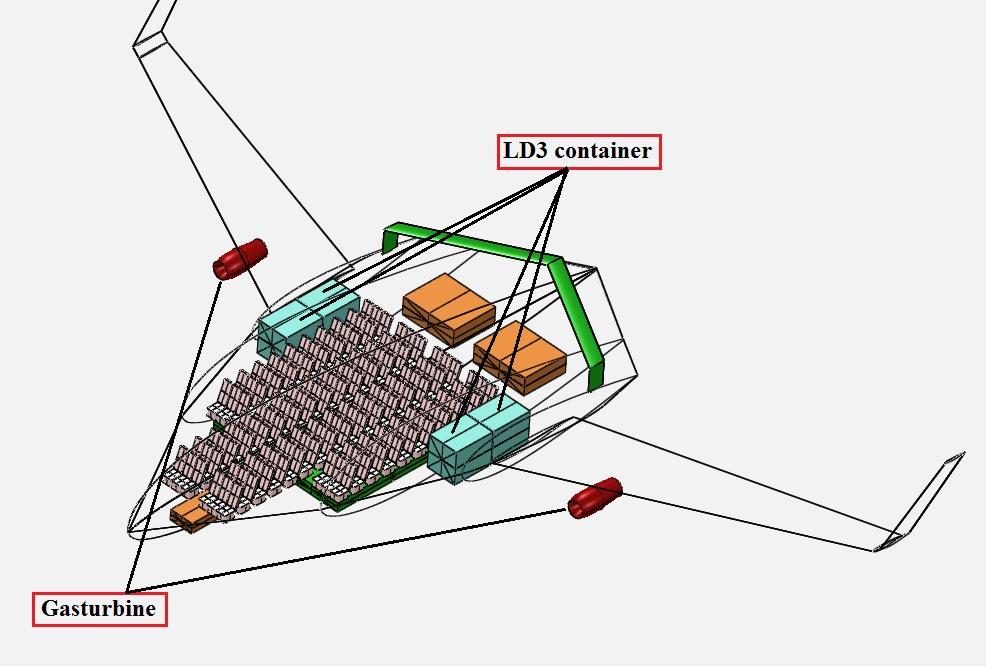
\includegraphics[keepaspectratio, width=\linewidth]{images/chap4/bwb_dep_render_upper.jpg}
		\caption{Upper surface.}
		\label{fig:bwb_dep_render_upper}
	\end{subfigure}
	\begin{subfigure}{0.6\textwidth}
		\centering
		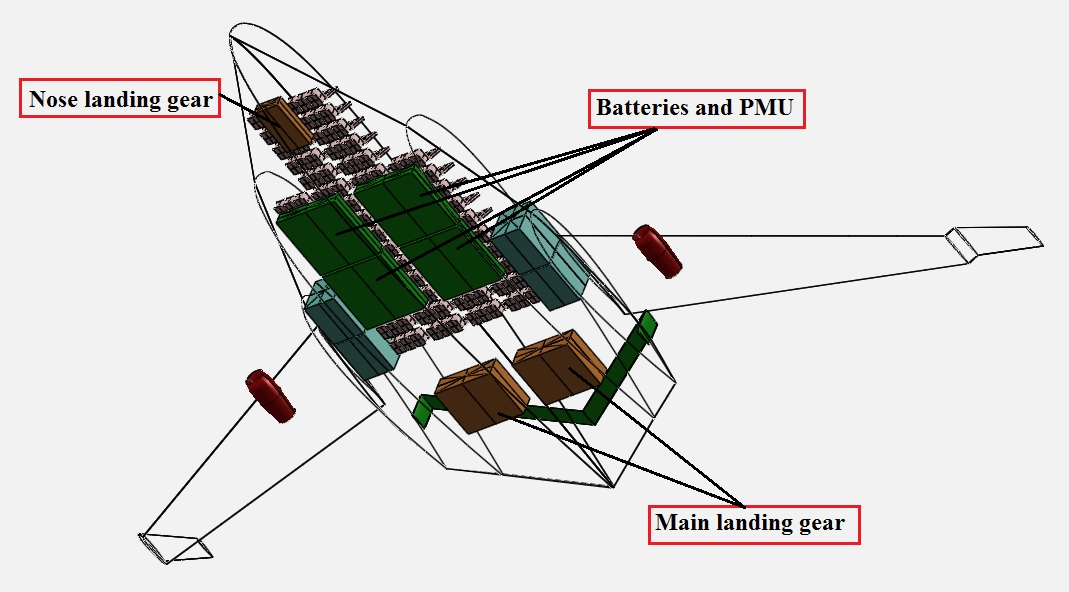
\includegraphics[keepaspectratio, width=\linewidth]{images/chap4/bwb_dep_render_lower.jpg}
		\caption{Lower surface.}
		\label{fig:bwb_dep_render_lower}
	\end{subfigure}
	\caption{Blended Wing-Body with distributed propulsion rendering, detail of subsystems allocation.}
	\label{fig:bwb_dep_render_detail}
\end{figure}

The transition zone is used to place the cargo. 
For 150 passengers, the maximum payload to be placed in the freight is 6000~\si{\kilogram}~\cite{bib:raymer, bib:airbus_notes}; in commerce different types of containers are available~\cite{bib:roskam_partIII}. 
Among the possibilities, the LD3 are here considered: they have maximum dimensions of $153\times164\times200$~\si{\centi\meter} for a total capacity of 1588~\si{\kilogram}, thus 4 of them are needed, as shown in Fig.~\ref{fig:bwb_dep_render_upper}. 
The width of transition zone $w_{tr}$ is fixed to 2~\si{\meter} to enable enough space to fit this type of containers.

Batteries and PMU are instead placed beneath the cabin.
They do not need a lot of volume and can be stretched, so they can fit in the volume available in that zone. 
Also, this positioning allows to forward the center of gravity, resulting in an outer wing advanced toward the leading edge, leaving space at the rear for boarding doors. 
Note that to make batteries work properly, this zone must be pressurised too.
In case the BWB uses conventional engines, the volume beneath the passengers cabin may be used for additional fuel tanks. 
The two gasturbines are placed beneath the wing: it is unusual to see engines in this position on a BWB, but among all the possibilities this one is the most reasonable.
In any case, the gasturbines are considerably smaller than a turbofan engine, and they can be allocated there without any drawbacks regarding the height from the ground. 

The landing gears are the remaining subsystems. 
Their dimensions are the same of the nose and main landing gear of the A320, increased of a percentage equals to the relative difference between the MTOW, to consider scaling effects.
The nose landing gear, which is more compact, is beneath the cockpit, where the airfoil rounded shape leaves space. 
The main landing is instead placed after the main spar, at 70\% of the chord. 
This position may not ensure enough rotational qualities at takeoff, but it is the only one possible.
It is to not forget that the BWB is more compact and shows a considerably smaller total length, so the center of gravity variation is not as wide as for the conventional aircraft. 
To tackle this issue, is assumed that the BWB can lift-off without rotation. 
This assumption will be verified during the sizing loop. 

Page et al.~\cite{bib:dzyne_bwb} developed a landing gear system that sets a virtual rotational point in order to ensure momentum at takeoff in all the conditions. 
Unfortunately, they do not provide details since it is a patent; in this research the assumption of takeoff without rotation, as for the B-52, is done. 

The description above has been done only considering the needing in volume for the main subsystems, but it does not present any detail on operations. 
For example, the cargo can be placed in the transition zone, but none has been said on the doors and systems to open and move containers. 
Same considerations are done for the batteries, that must be removed and inserted easily between one mission and another. 
These operations require cute-off, that must be properly sized, and weaken the structure. 
Future work on a more detailed design can not prescind by these aspects. 

Next section will finally present the integration of all the methods developed in the sizing procedure, to design a BWB, and the further implementation of the MDA in an optimisation loop. 

\section{Methodology for the Blended Wing-Body sizing}
\label{sec:chap4_bwb_sizing}

\subsection{MDA sizing loop}
\label{subsec:chap4_bwb_mda}

The revised sizing loop, tailored for the BWB, is shown in Fig.~\ref{fig:fast_mda_bwb}, with the detailed algorithm reported in Alg.~\ref{alg:fast_mda_bwb}.
Note that, as intermediate step, the MDA presented here is intended to design a BWB with conventional propulsion; the hybrid architecture will be added later on.
\begin{figure}[!h]
	\centering
	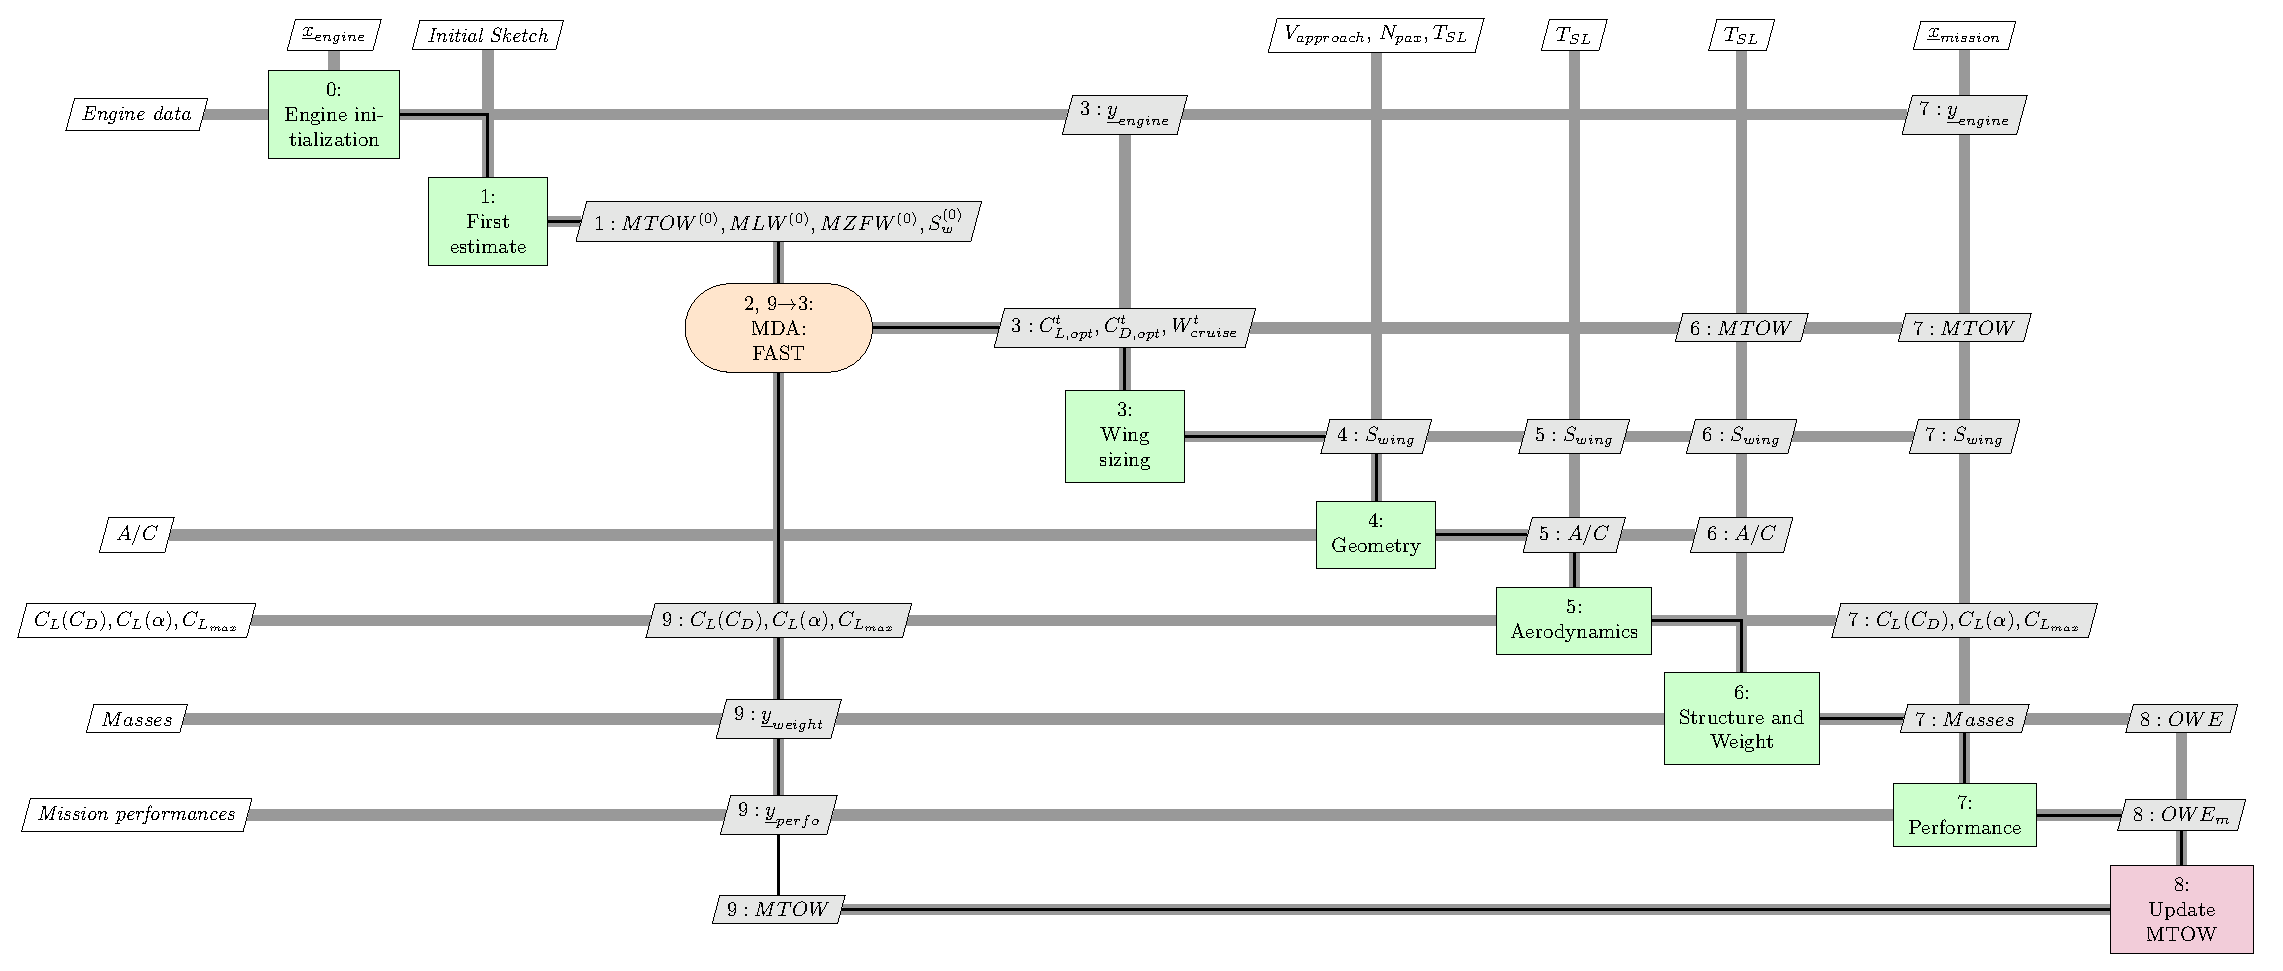
\includegraphics[keepaspectratio, width=1.3\textwidth, angle=90]{images/chap4/FAST_MDA_BWB}
	\caption{MDA loop tailored for the Blended Wing-Body sizing with conventional propulsion.}
	\label{fig:fast_mda_bwb}
\end{figure}

\begin{algorithm}[!h]
	\caption{FAST algorithm, tailored for the BWB sizing with conventional propulsion. Numbering is referred to Fig.~\ref{fig:fast_mda_bwb}.}
	\label{alg:fast_mda_bwb}
	\begin{algorithmic}
		\REQUIRE Initial design parameters (TLAR)
		\ENSURE Sized aircraft, drag polars, masses, design mission trajectory
		\STATE 0: Engine initialization.
		\STATE 1: First estimate of top level parameters, such as wing area, OWE and MTOW.
		\STATE 2: Initialise the sizing loop.
		\REPEAT
		\STATE 3: Wing area sizing. For the BWB the wing area is intended as total planform area.
		\STATE 4: Geometry is obtained and then resized to match stability constraint, according to the parametrization described in Sec.~\ref{subsec:chap4_bwb_arrangement}.
		\STATE 5: Aerodynamics calculation. Here corrective factors to adjust data with high fidelity are applied.
		\STATE 6: Mass breakdown analysis..
		\STATE 7: Performance calculation.
		\STATE 8: Update the value of MTOW, with the data coming from analyses 5 and 7, according to Eq.~\eqref{eq:mtow_new}.
		\STATE 9: Check the convergence: if the tolerance is below the needed thresold, return the sized aircraft, otherwise proceed to next iteration.
		\UNTIL {$9 \rightarrow 3$: MDA has converged}
	\end{algorithmic}
\end{algorithm}

The xDSM scheme illustrated in Fig.~\ref{fig:fast_mda_bwb} does not differ greatly from that one of Fig.~\ref{fig:fast_basic}. 
Indeed, the global procedure is always the same, at least regarding the call of analyses.
The differences are in the modules adopted, that are tailored for the BWB, as described in previous sections. 

The wing area, called at step 3, is also changed: it is to recall that a conventional aircraft must comply with approach condition and fuel stored, but these criteria may not be suitable for a BWB. 
Just as example, with the data of the BWB reference geometry reported in Table~\ref{tab:bwb_ref_geometry_tlar} the surface computed with the approach condition results to be around 150~\si{\square\meter}, as the planform reference area is 313~\si{\square\meter}. 

To understand what is the proper condition, a constraint analysis is carried out~\cite{bib:roskam_partI}. 
This analysis gives as output the plot of thrust to weight as function of wing loading for different flight conditions. 
In particular, the criteria considered are:
\begin{itemize}
	\item Approach constraint, to supply enough lift in this phase;
	\item Takeoff constraint, to ensure that the aircraft can depart in a prescribed runway length;
	\item Initial climb constraint, to ensure that at 400~ft and in OEI condition the climb rate is at least 2.4\%;
	\item Top of climb constraint, to ensure that the aircraft has a reserve of vertical speed of 300 ft\si{\per\minute};
	\item Geometrical constraint, in order to guarantee the total area is greater than the centerbody area only;
	\item Span constraint, which is limited to 36~\si{\meter} for this category of aircraft. 
\end{itemize}

The constraint diagram for the BWB is shown in Fig.~\ref{fig:bwb_constraint_analysis}; reference mass is the MTOW, thrust is intended at sea level. 
On a conventional aircraft, for short and medium range the top of climb condition is not so relevant in the design; contrarly for the BWB it becomes the main limitation at the design space.
\begin{figure}[!h]
	\centering
	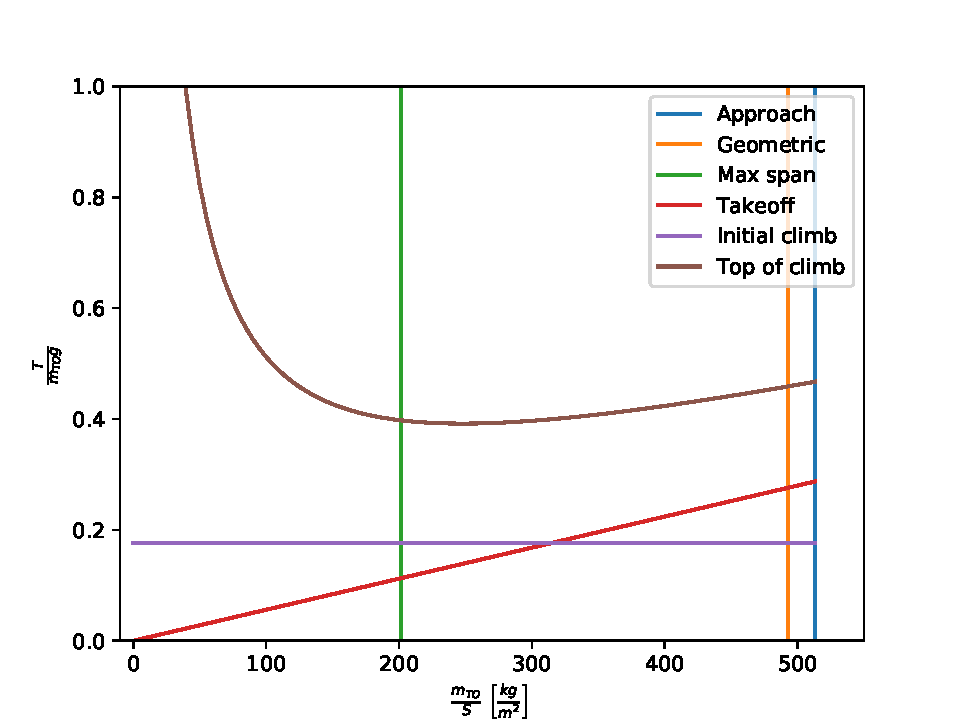
\includegraphics[keepaspectratio, width=0.6\textwidth]{images/chap4/bwb_constraint_analysis}
	\caption{Constraint diagram for the BWB with conventional propulsion.}
	\label{fig:bwb_constraint_analysis}
\end{figure}
It is also to note that the approach condition can not be the right one because the resulting area is lower than that of the centerbody. 
Another remarkable point regards the optimum point: the top of climb condition shows a minimum, which corresponds to the maximum LoD value at that point. 
Thus, at step 2 the top of climb condition replaces the approach condition for the BWB.

Geometry, aerodynamics and mass breakdown modules are modified to consider the models and correction developed in Sec.~\ref{sec:chap4_bwb_modeling}. 
Parametrization shown in Fig.~\ref{fig:bwb_planform_scheme} is used; for the vertical tail same methods as for the TAW concept are applied, with the only difference that for a BWB there are two surfaces in place of one, corresponding to the two winglets. 
Performance module and convergence criteria are not modified. 

The next step is finally the definition of an MDO formulation for the Blended Wing-Body with distributed electric propulsion.

\subsection{MDO formulation}
\label{subsec:chap4_bwb_mdo}

The MDA represents an intermediate step to ensure the BWB sizing procedure works; it also allows to assess the advantage of the BWB solely, without the integration with distributed propulsion. 

The final integration of the DEP into a BWB architecture can be easily obtained at this point of the research. 
In fact, all the individual modules for the BWB sizing and the DEP are ready, and thanks to the modular approach they can be directly inserted in the MDF architecture, replacing the old one. 

The resulting procedure is identical to what has been shown in Fig.~\ref{fig:fast_openmdao_dep} and described in Alg.~\ref{alg:fast_openmdao_dep}, with the modules regarding geometry, aerodynamics and structure tailored for the BWB replace the ones for conventional aircraft. 
The performance is not modified: in fact for this analysis aircraft is described as just a point with mass and aerodynamics properties, and it works fine for all the configurations as far mass and aerodynamics are valid. 

This procedure will be applied in next section to optimise and evaluate performances of BWB featuring DEP. 

\section{The Blended Wing-Body featuring conventional propulsion}
\label{sec:chap4_bwb_mda_results}

\subsection{Design mission analysis}
\label{subsec:chap4_bwb_mda_design_mission}

In this section performance for the BWB featuring conventional propulsion are evaluated, considering the same TLAR as the A320 reference aircraft, reported in Table~\ref{tab:fast_base_tlar}. 

The EIS2035 is considered, so the same assumptions done on structure and aerodynamics and reported in Table~\ref{tab:2035_mass_impact} and Table~\ref{tab:2035_aero_impact} respectively are retained.
The only difference is that no reduction for the fuselage (equivalent to centerbody) is considered, since the use of new material is already contained in Eq.~\eqref{eq:bwb_cabin_mass}.
Also regarding the propulsion, two LEAP type engines~\cite{bib:leap_engine} at the trailing edge are considered. 

The geometrical inputs adopted are reported in Table~\ref{tab:bwb_conv_geom_inp}: for the BWB, the subscript $out$ indicates the outer wing only, meanwhile the subscript $w$ refers to global parameters.
The minimum centerbody height is 2.18~\si{\meter} as explained in Sec.~\ref{subsec:chap4_bwb_arrangement}; also to remark that thickness-to-chord ratio for outer wing is a mean value: in real, it is thicker at root and thiner at tip. 
\begin{table}[!h]
	\centering
	\begin{tabular}{l c}
		\hline
		$AR_w$ & 3.2 \\
		$\Lambda_{LE_{cb}}$ & 45~\si{\deg} \\
		$\lambda_{cb}$ & 0.65 \\
		$\lambda_{tr}$ & 0.8 \\
		$\Lambda_{25_{out}}$ & 25~\si{\deg} \\
		$\left(\frac{t}{c}\right)_{out}$ & 0.1 \\
		$\lambda_{out}$ & 0.3 \\
		\hline
	\end{tabular}
	\caption{Geometrical inputs for the BWB with conventional propulsion sizing case.}
	\label{tab:bwb_conv_geom_inp}
\end{table}

The BWB aircraft is compared with A320 case study, resized to consider the same EIS2035. 
Results for the design mission are reported in Table~\ref{tab:bwb_conv_results}. 
The BWB shows a heavier structure, which results in a greater MTOW, as expected because of the complexity of the structure. 
Nevertheless, the maximum LoD value is increased of 30\%: the improved aerodynamics counterbalance the penalties in mass, and finally the fuel consumption is reduced of about 13\%. 
\begin{table}[!h]
	\centering
	\begin{tabular}{l l c c}
		\cline{3-4}
		& & \textbf{Baseline} & \textbf{BWB} \\
		\hline
		\textbf{MTOW} & [\si{\tonne}] & 68.3 & 73.9 \\
		\textbf{OWE} & [\si{\tonne}] & 40.9 & 48.4 \\
		\textbf{Wing area} & [\si{\square\meter}] & 120.37 & 395.06 \\
		\textbf{Max. LoD} & & 17.02 & 22.92 \\
		\textbf{Cruise altitude} & [kft] & 34.6 & 38.9 \\
		\textbf{Fuel mission} & [\si{\tonne}] & 13.6 & 11.8 \\
		\hline
		\textbf{CAT.POL.A.410(a)-1} & [ft\si{\per\minute}] & 947.36 & 640.97 \\
		\textbf{CAT.POL.A.410(a)-2} & [ft\si{\per\minute}] & 736.79 & 633.95 \\
		\textbf{CS-25.119(a)} & [\%] & 21.52 & 12.27 \\
		\textbf{CS-25.121(a)} & [\%] & 3.66 & 0.79 \\
		\textbf{CS-25.121(b)} & [\%] & 5.53 & 4.28 \\
		\textbf{CS-25.121(c)} & [\%] & 6.96 & 7.46 \\
		\textbf{CS-25.121(d)} & [\%] & 8.41 & 2.12 \\
		\hline		
	\end{tabular}
	\caption{Comparison between the A320 resized to match EIS2035 and the BWB, with the TLAR reported in Table~\ref{tab:fast_base_tlar}.}
	\label{tab:bwb_conv_results}
\end{table}
The centerbody relative thickness is about 0.19: despite the value still makes the airfoil theory valid~\cite{bib:abbott}, it is higher than other BWB in literature, which suggest values around 0.15~\cite{bib:van_dommelen, bib:bwb_n3_vol1}. 
Indeed, the BWB examples found in literature are for very large passengers and long range (competitor of \textit{i.e.} Boeing 777): for these geometries the chord are greater, and this lead to a reduced relative thickness. 
The size of the BWB here considered is smaller, and thus the centerbody is thicker. 
Higher relative thickness may be problematic in transonic, since it facilitates the formation of shock wave; a careful aerodynamics design is needed as further step. 
Regarding the certification, from Table~\ref{tab:bwb_conv_results} comes out also that, even if the BWB complies with all the CS-25, the performances are worse than the conventional aircraft, except for the CS-25.121(c). 

Another feature concerns the cruise altitude, which is higher than the conventional aircraft. 
In some way, this has already been detected in Sec.~\ref{subsec:chap4_bwb_aero_cfd}, where it is mentioned that the first estimate of cruise altitude is underestimating the real value. 
For a BWB, indeed, the wing loading is lower than for a reference aircraft:
\begin{equation}
	\label{eq:wing_loading_bwb_ref_comp}
	\left(\frac{m}{S_w}\right)_{BWB} < \left(\frac{m}{S_w}\right)_{ref}
\end{equation}
Let consider the $C_L$ equation, described in Eq.~\eqref{eq:lift_equation}. 
Replacing the velocity by its definition $V=Ma_{\infty}$ it is possible to manipulate the equation to put in evidence the wing loading:
\begin{equation}
	\label{eq:cl_manipulated}
	C_L = \left(\frac{m}{S_{w}}\right)\frac{2g}{\rho M^2a_{\infty}^2}
\end{equation} 
The combination of Eq.~\eqref{eq:cl_manipulated}, written for the BWB and the reference aircraft, with the condition \eqref{eq:wing_loading_bwb_ref_comp} yields to 
\begin{equation}
	\label{eq:cl_rewritten}
	\frac{C_{L_{BWB}}}{C_{L_{ref}}} < \frac{\rho_{ref}a_{\infty_{ref}}^2}{\rho_{BWB}a_{\infty_{BWB}}^2}
\end{equation}
In case of the BWB, because of the greater area, the $C_L$ in cruise (that is recalled, is equal to the optimal $C_L$) is smaller than the reference aircraft, as depicted in Fig.~\ref{fig:bwb_polar_comp}, that shows the comparison of the cruise polars for the BWB and the reference aircraft.
\begin{figure}[!h]
	\centering
	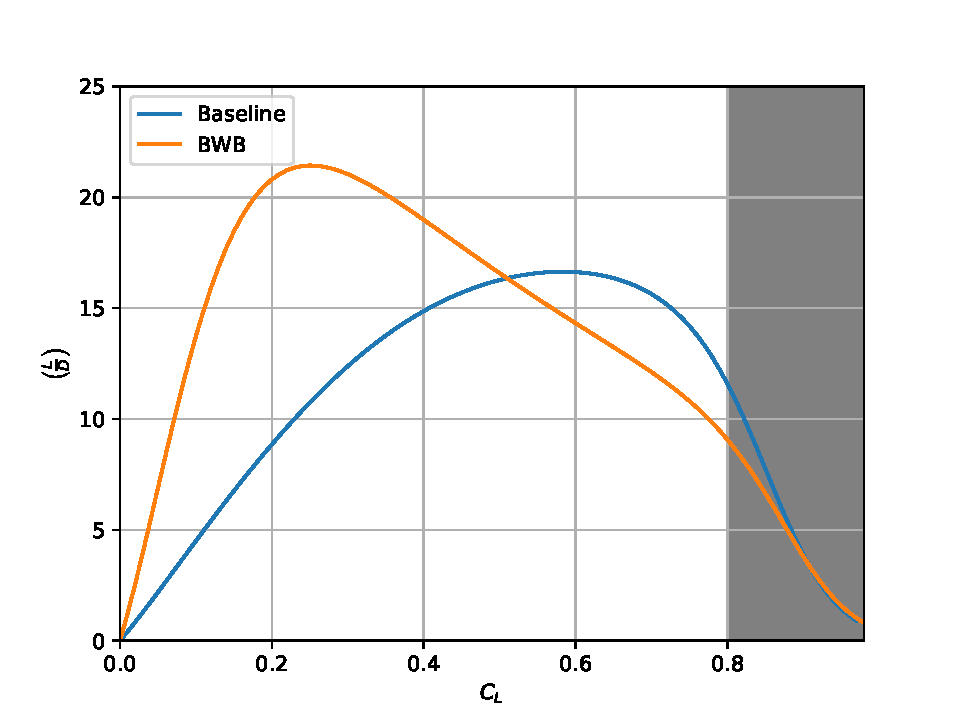
\includegraphics[keepaspectratio, width=0.6\textwidth]{images/chap4/bwb_conv_polar_comparison}
	\caption{Comparison between the LoD curve for the reference aircraft and the BWB with conventional propulsion. Shading identifies the region where models are not accurate anymore, since the wave drag is not well predicted at high $C_L$.}
	\label{fig:bwb_polar_comp}
\end{figure}
This yields to conclude that, to satisfy the condition \eqref{eq:cl_rewritten}, the following relation holds:
\begin{equation}
	\label{eq:cl_cond_bwb_ref}
	\rho_{BWB}a_{\infty_{BWB}}^2 < \rho_{ref}a_{\infty_{ref}}^2
\end{equation}
The inequality expressed in \eqref{eq:cl_cond_bwb_ref} is verified only if the BWB flies at higher altitude, since both the density and the speed of sound decrease with this quantity. 
Therefore, it is explained the result noted in Table~\ref{tab:bwb_conv_results}.
The increased altitude may be an issue since for the BWB the actual rules for the routes and their management most likely need to be revised, to allow BWB flying at specified flight level. 
Also, the implication of the cruise altitude on the pollution level must be assessed. 

Finally, the mass breakdown is illustrated in Fig.~\ref{fig:bwb_conv_mb}.
\begin{figure}[!h]
	\centering
	\begin{subfigure}{0.45\textwidth}
		\centering
		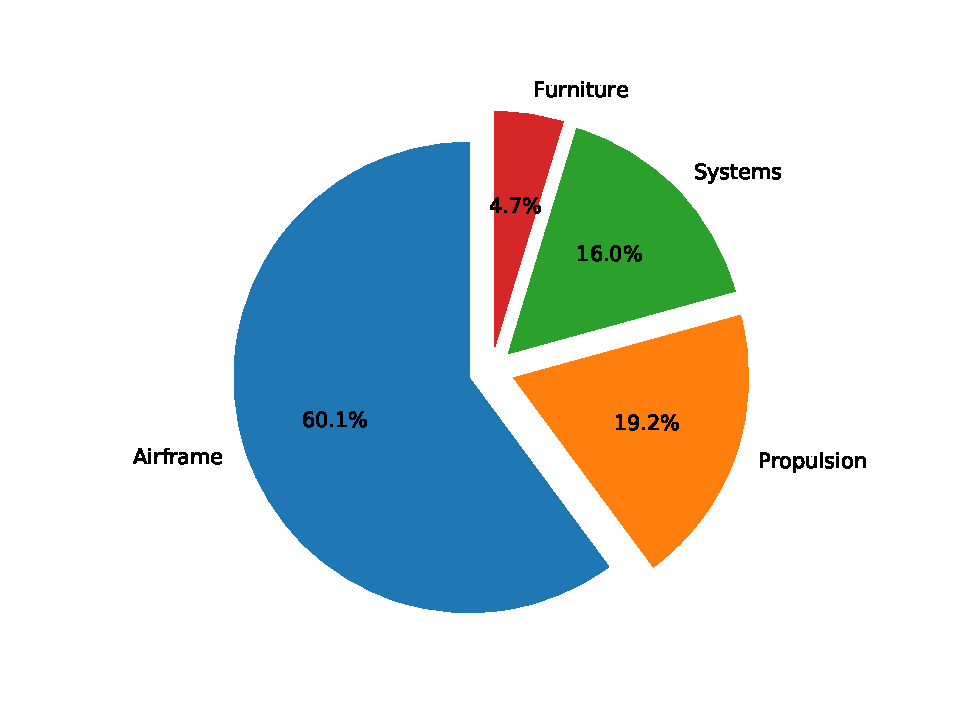
\includegraphics[keepaspectratio, width=\linewidth]{images/chap4/bwb_conv_mb}
		\caption{Global breakdown.}
		\label{fig:bwb_conv_mb_global}
	\end{subfigure}
	\begin{subfigure}{0.45\textwidth}
		\centering
		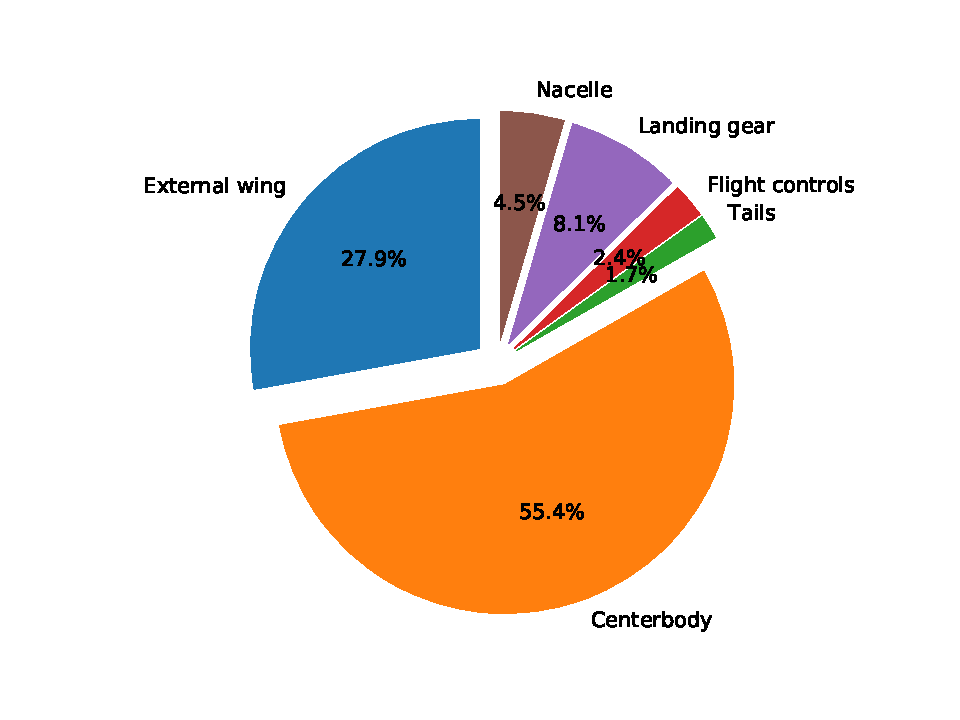
\includegraphics[keepaspectratio, width=\linewidth]{images/chap4/bwb_conv_airframe_mb}
		\caption{Airframe detail.}
		\label{fig:bwb_conv_mb_detail_airframe}
	\end{subfigure}
	\caption{Mass breakdown for the BWB featuring conventional propulsion, with TLAR reported in Table~\ref{tab:fast_base_tlar}. Mass norm is the reference French 2001/D, used in FAST~\cite{bib:mass_breakdown}.}
	\label{fig:bwb_conv_mb}
\end{figure}
It is the airframe, indeed, that accounts for the most of structural weight (about 60\%); of this percentage, the centerbody represents more than half of the total weight, as expected. 
The outer wing accounts for a 30\%, meanwhile the rest is equally divided by other components. 
Percentages are in line with values coming from internal work at ONERA, on the CICAV project~\cite{bib:defoort}, and other examples in literature~\cite{bib:van_dommelen}, despite the type is different.

\subsection{Operational area assessment}
\label{subsec:chap4_bwb_mda_operational}

The analysis of the BWB concept continues with an assessment of its performance in operational points. 
Indeed, for airlines, it is interesting to have aircraft efficient in different conditions, not only that of design. 
During the life cycle aircraft, in fact, very rarely it flies at its design range. 
For this reason, studies on the performance on other ranges than that of design have been carried out. 

The ranges vary between 600 and 2200~nmi; results for the BWB and the baseline are shown in Fig.~\ref{fig:bwb_op_range_comp}.
\begin{figure}[!h]
	\centering
	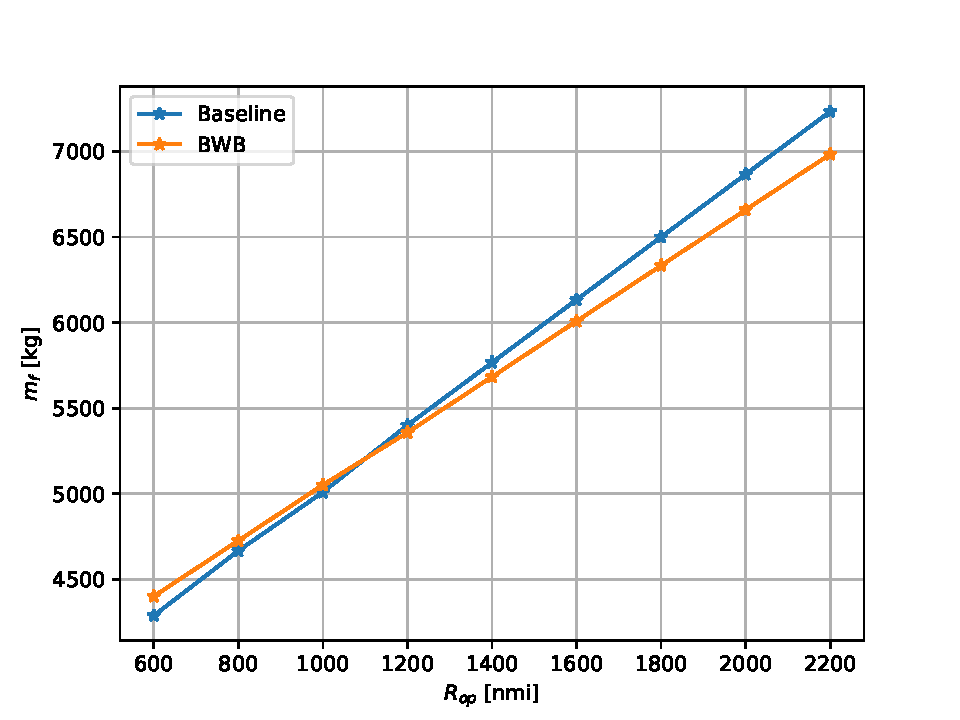
\includegraphics[keepaspectratio, width=0.6\textwidth]{images/chap4/bwb_op_range_comp}
	\caption{Comparison between the reference aircraft and the BWB with conventional propulsion for different operational ranges.}
	\label{fig:bwb_op_range_comp}
\end{figure}
From the diagram, it comes out that the BWB is more efficient for longer ranges, but at lower distances the baseline saves more fuel. 
This is linked to the comment done in previous section on the flight altitude for the BWB. 
Indeed, the disruptive concept needs to climb higher, which takes more time; specifically 31~\si{\minute} in place of 25~\si{\minute}.
The engine model is the same for both aircraft, as well as the climb profile (in terms of CAS). 
Neglecting variations of thrust and SFC for the last phase of BWB climb (after it passes the cruise altitude of the reference aircraft) and recalling that $dm_f=\textrm{T(SFC)}dt$, it can be concluded that the ratio between the fuel consumption of the two aircraft is equal to the ratio between the time of climb.
This means that, with numeric values given, the BWB consumes approximately 20\% more fuel than the reference aircraft. 
On short distances, this quantity is not counterbalanced by the reduced FC in cruise, because of the shorteness of this segment. 
This explains also why in literature most of the BWB concepts so far refer to long and very long range.  

Finally, the Payload-Range curve is also obtained. 
Two different conditions have been taken into account for the BWB. 
The volume beneath the cabin is empty in this case, whereas no batteries are included (as in Fig.~\ref{fig:bwb_dep_render_upper}), and it may be used for additional tanks.
The amount of fuel stored is estimated by the knowledge of the volume and the density. 

The Payload-Range, considering additional tanks and not, is shown in Fig.~\ref{fig:bwb_pl_range}, compared with the baseline diagram. 
The maximum distance can be travelled at maximum payload is reduced for the BWB by about 200~nmi, because as said the concept is not competitive against the conventional TAW on short ranges.
\begin{figure}[!h]
	\centering
	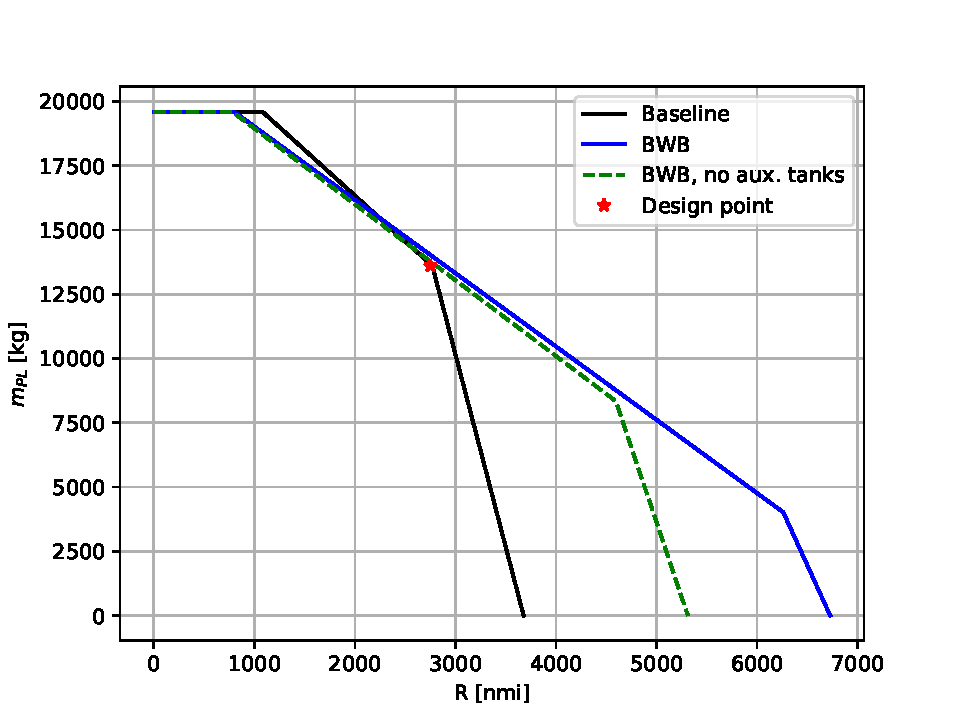
\includegraphics[keepaspectratio, width=0.6\textwidth]{images/chap4/bwb_pl_range}
	\caption{Payload-Range comparison between the reference aircraft and the BWB with conventional propulsion, considering the two cases with auxiliary tanks and not.}
	\label{fig:bwb_pl_range}
\end{figure}
On the contrary, for longer distance the performances of BWB are so improved that ferry range is increased of about 1400~nmi in the case with no additional tanks, and almost 3000~nmi with additional tanks. 
The difference in MFW with and without tanks in the centerbody is of 6~\si{\tonne}. 
This value alone can not explain a range increased of about 1600~nmi, but it is to not forget that mass is decreasing going on right, and so the mass is reduced not linearly but there is a combined effect. 

Now that the BWB performances are well assessed, considering conventional engines, it is possible to pass to the exploration of the BWB with DEP, final objective of the research. 

\section{The Blended Wing-Body with distributed electric propulsion}
\label{sec:chap4_bwb_mdo_results}

\subsection{Problem formulation}
\label{subsec:chap4_bwb_optim_prob}

The problem statement for the optimisation of BWB with distributed electric propulsion is synthesized in Table~\ref{tab:bwb_hybrid_dep_problem_optimisation_definition}. 
\begin{table}[h!]
	\centering
	\begin{tabular}{l l r r r r l}
		\hline
		\textbf{Category} & \textbf{Name} & \textbf{Size} & \textbf{Lower} & \textbf{Upper} & \textbf{Equals} & \textbf{Units} \\
		\hline
		Objective & $f\left(\underline{x}\right)$ & 1 & -- & -- & -- & -- \\
		\hline
		Variables & $S_w$ & 1 & \num{250} & \num{450} & -- & \si{\square\meter} \\
		& $x_{out}$ & 1 & \num{12} & \num{16} & -- & \si{\meter} \\
		& $AR_{w}$ & 1 & \num{2.5} & \num{5} & -- & -- \\
		& $\Lambda_{LE_{cb}}$ & 1 & \num{30} & \num{60} & -- & \si{\deg} \\
		& $\lambda_{cb}$ & 1 & \num{0.5} & \num{0.8} & -- & -- \\
		& $\left(\frac{t}{c}\right)_{cb}$ & 2 & \num{0.15} & \num{0.24} & -- & -- \\
		& $\lambda_{tr}$ & 1 & 0.6 & 0.8 & -- & -- \\
		& $\lambda_{out}$ & 1 & \num{0.2} & \num{0.6} & -- & -- \\
		& $\Lambda_{25_{out}}$ & 1 & \num{20} & \num{45} & -- & \si{\deg} \\
		& $\left(\frac{t}{c}\right)_{out}$ & 1 & \num{0.1} & \num{0.15} & -- & -- \\
		& $S_{VT}$ & 1 & \num{15} & \num{50} & -- & \si{\square\meter} \\
		& $AR_{VT}$ & 1 & \num{1} & \num{2.5} & -- & -- \\
		& $\lambda_{VT}$ & 1 & \num{0.85} & \num{1.0} & -- & -- \\
		& $\Lambda_{25_{VT}}$ & 1 & \num{25} & \num{55} & -- & \si{\deg} \\
		& $\left(\frac{t}{c}\right)_{VT}$ & 1 & \num{0.1} & \num{0.15} & -- & -- \\
		& $k_{GT}$ & 1 & \num{0.5} & \num{1.5} & -- & -- \\
		& $P_{400}$ & 1 & \num{6} & \num{18} & -- & \si{\mega\watt} \\
		& $\tau_{b}$ & 1 & \num{1} & \num{3} & -- & \si{\cubic\meter} \\
		& FPR & 1 & \num{1.05} & \num{1.4} & -- & -- \\
		& $h_{toc}$ & 1 & \num{32000} & \num{42000} & -- & ft \\
		& \textbf{Total} & 21 & & & & \\
		\hline
		Constraints & $\Delta m_{f}$ & 1 & 0 & -- & -- & \si{\kilogram} \\
		& $b_w$ & 1 & -- & \num{36} & -- & \si{\meter} \\
		& $y_t$ & 2 & 2.18 & -- & -- & \si{\meter} \\
		& $\Delta \mathcal{N}_{cruise}$ & 1 & \num{0} & -- & -- & \si{\newton\meter} \\
		& $\Delta P_{b}$ & 1 & \num{0} & -- & -- & \si{\watt} \\
		& $\Delta l_{nac}$ & 1 & -- & \num{0} & -- & \si{\meter} \\
		& $\bar{r}_f$ & 1 & -- & \num{0.05} & -- & -- \\
		& TOFL & 1 & -- & \num{2200} & -- & \si{\meter} \\
		& SM & 1 & \num{0} & \num{0.05} & -- & -- \\
		& $\tan \gamma_{400}$ & 1 & \num{0.024} & -- & -- & -- \\
		& $\underline{c}_{CCM}$ & 5 & \num{0} & -- & -- & \% \\
		& $SoC_f$ & 1 & -- & -- & \num{0.20} & -- \\
		& $\Delta C_{L_{toc}}$ & 1 & -- & -- & 0 & -- \\
		& \textbf{Total} & 18 & & & & \\
		\hline    	
	\end{tabular} 
	\caption{Optimisation problem definition for the BWB aircraft with distributed electric propulsion case.}
	\label{tab:bwb_hybrid_dep_problem_optimisation_definition}
\end{table}
Besides the bounds of variables that are of course adapted to the BWB case, only minor differences are present, compared to previous case of the hybrid aircraft optimisation problem reported in Table~\ref{tab:hybrid_dep_problem_optimisation_definition}.
\begin{itemize}
	\item The parameters to define the centerbody are included in the design variables, according to the parametrization reported in Fig.~\ref{fig:bwb_planform_scheme}. 
	Note that the relative thickness has size 2, because the constraint on the height $y_t$ is evaluated at symmetry and outmost plane;
	
	\item The horizontal tail parameters are removed, since the BWB is a tailless aircraft;
	
	\item The approach condition is replaced by the condition of minimum vertical speed at top of climb, as emerges from Fig.~\ref{fig:bwb_constraint_analysis}. 
	The limits for the cruise altitude are augmented of 2000~ft in agreement with the peculiarity of the BWB that flies higher;
	
	\item The lower limit for fan over chord ratio $\bar{r}_f$ is reduced to 0.05, because of the MAC which is more than doubled with respect to conventional aircraft;
	
	\item The static margin limits are reduced, in agreement with the discussion done in Sec.~\ref{subsubsec:chap4_bwb_sensitivity_sm}.
\end{itemize}

In total, the problem consists of 20 design variables subject to 17 design constraints (2 equalities and 15 inequalities). 

As usual, before going through the optimisation of the BWB, a sensitivity analysis is presented, both to understand the impact of variables on overall design and to eventually reduce the size of the optimisation problem.

\subsection{Sensitivity analysis results}
\label{subsec:chap4_bwb_sens_an}

As already done for the TAW with distributed propulsion, before going through the process of optimisation a sensititivity analysis is performed, using the PCE method (see Appendix~\ref{app:pce_method} for more details).

In a similar way than the previous case, the wing and vertical tail surfaces, as well as the wing position and the cruise altitude are not considered, since it is not of interest to analyse their impact, being directly subject to design constraints and then not free to be modified by designer. 
Also, the battery volume is recomputed according to Eq.~\eqref{eq:battery_volume_soc} to ensure for all points a final SoC equals to 0.20. 

Concerning the other variables, the design space is defined together with the problem in Table~\ref{tab:bwb_hybrid_dep_problem_optimisation_definition}; the configuration chosen for sensitivity corresponds to R~=~900~nmi and $N_{EM}=32$.  

The design of experiments consists of 800 points, whereas 750 belong to training set, and the remaining to the validation set. 
As usual, Sobol indices are computer for energy consumption $E_c$, battery volume $\tau_{b}$, OWE $m_e$, maximum LoD value $\left(\frac{L}{D}\right)_{\max}$ and static margin SM.

Table~\ref{tab:bwb_hybrid_dep_sens_an_geom_sobol} presents first order Sobol indices mean value $\mu$, meanwhile Table~\ref{tab:bwb_hybrid_dep_sens_an_geom_cv} reports the relative coefficients of variation; with the convention that in case the mean value $\mu$ is zero, coefficient of variation $\sigma^{\star}$ is replaced by its variance. 
An asterisk indicates the case where the convention is applied.
\begin{table}[!h]
	\centering
	\begin{tabular}{l c c c c c}
		\hline
		& $E_{c}$ & $\tau_{b}$ & $m_e$ & $\left(\frac{L}{D}\right)_{\max}$ & SM \\
		\hline
		$AR_w$ & $\mathbf{6.82\times10^{-1}}$ & $2.65\times10^{-2}$ & $\mathbf{5.21\times10^{-1}}$ & $\mathbf{9.03\times10^{-1}}$ & $2.33\times10^{-2}$ \\
		$\lambda_{out}$ & $3.31\times10^{-3}$ & $8.41\times10^{-4}$ & $1.99\times10^{-2}$ & $2.87\times10^{-4}$ & $3.26\times10^{-2}$ \\
		$\left(\frac{t}{c}\right)_{out}$ & $3.39\times10^{-2}$ & $1.72\times10^{-2}$ & $5.13\times10^{-3}$ & $9.98\times10^{-5}$ & $2.70\times10^{-2}$ \\
		$\Lambda_{25_{out}}$ & $3.14\times10^{-2}$ & $1.80\times10^{-2}$ & $3.39\times10^{-2}$ & $9.38\times10^{-4}$ & $\mathbf{1.34\times10^{-1}}$ \\
		
		$\Lambda_{LE_{cb}}$ & $7.04\times10^{-3}$ & $5.88\times10^{-4}$ & $\mathbf{1.49\times10^{-1}}$ & $1.06\times10^{-2}$ & $\mathbf{2.12\times10^{-1}}$\\
		$\left(\frac{t}{c}\right)_{cb}$ & $3.14\times10^{-2}$ & $1.54\times10^{-3}$ & $5.11\times10^{-3}$ & $1.42\times10^{-2}$ & $2.98\times10^{-2}$\\
		$\lambda_{cb}$ & $1.35\times10^{-2}$ & $8.63\times10^{-4}$ & $1.25\times10^{-2}$ & $2.11\times10^{-3}$ & $\mathbf{1.56\times10^{-1}}$ \\
		$\left(\frac{t}{c}\right)_{tr}$ & $5.01\times10^{-3}$ & $1.97\times10^{-4}$ & $3.21\times10^{-3}$ & $1.35\times10^{-3}$ & $3.78\times10^{-2}$ \\
		$\lambda_{tr}$ & $5.01\times10^{-3}$ & $2.64\times10^{-2}$ & $3.72\times10^{-2}$ & $1.84\times10^{-4}$ & $3.22\times10^{-2}$ \\
		
		$AR_{VT}$ & $3.69\times10^{-3}$ & 0 & $2.34\times10^{-3}$ & $6.15\times10^{-4}$ & $3.38\times10^{-2}$ \\
		$\lambda_{VT}$ & $2.96\times10^{-3}$ & 0 & $2.38\times10^{-3}$ & $2.91\times10^{-4}$ & $2.42\times10^{-2}$ \\
		$\left(\frac{t}{c}\right)_{VT}$ & $3.50\times10^{-3}$ & $6.94\times10^{-5}$ & $3.79\times10^{-3}$ & $4.39\times10^{-4}$ & $3.24\times10^{-2}$ \\
		$\Lambda_{25_{VT}}$ & $4.12\times10^{-3}$ & 0 & $3.05\times10^{-3}$ & $1.17\times10^{-3}$ & $2.31\times10^{-2}$ \\
		
		FPR & $\mathbf{1.34\times10^{-1}}$ & $\mathbf{9.07\times10^{-1}}$ & $\mathbf{1.56\times10^{-1}}$ & $6.16\times10^{-2}$ & $2.17\times10^{-2}$ \\
		\hline
		\textbf{Sum} & $9.66\times10^{-1}$ & $9.76\times10^{-1}$ & $9.56\times10^{-1}$ & $9.96\times10^{-1}$ & $7.89\times10^{-1}$ \\
		\hline
	\end{tabular}
	\caption{First order Sobol indices mean value $\mu$ for key output variables with respect to inputs, BWB with distributed electric propulsion case. 
		Most relevant parameters for each output are written in bold.}
	\label{tab:bwb_hybrid_dep_sens_an_geom_sobol}
\end{table}
\begin{table}[!h]
	\centering
	\begin{tabular}{l c c c c c}
		\hline
		& $E_{c}$ & $\tau_{b}$ & $m_e$ & $\left(\frac{L}{D}\right)_{\max}$ & SM \\
		\hline
		$AR_w$ & $1.22\times10^{-1}$ & 1.41 & $2.21\times10^{-1}$ & $4.96\times10^{-2}$ & 5.47 \\
		$\lambda_{out}$ & 9.24 & $2.17\times10$ & 1.79 & $2.25\times10$ & 3.60 \\
		$\left(\frac{t}{c}\right)_{out}$ & 1.12 & 1.86 & $4.75\times10^{-1}$ & $7.76\times10$ & 4.89 \\
		$\Lambda_{25_{out}}$ & 1.18 & 1.84 & 4.56 & 9.98 & $2.28\times10^{-1}$ \\
		
		$\Lambda_{LE_{cb}}$ & 4.35 & $3.07\times10$ & $4.39\times10^{-2}$ & 3.10 & 1.08 \\
		$\left(\frac{t}{c}\right)_{cb}$ & 1.03 & $1.29\times10$ & 8.60 & 1.39 & 4.57 \\
		$\lambda_{cb}$ & 2.58 & $2.26\times10$ & 4.60 & $1.21\times10$ & 1.16 \\
		$\left(\frac{t}{c}\right)_{tr}$ & 5.14 & $7.62\times10$ & $1.28\times10$ & 8.28 & 3.36 \\
		$\lambda_{tr}$ & 2.53 & 8.42 & 1.00 & $4.79\times10$ & 3.59 \\
		
		$AR_{VT}$ & 6.76 & 0\textsuperscript{*} & $1.62\times10$ & $1.45\times10$ & 3.69 \\
		$\lambda_{VT}$ & 8.47 & 0\textsuperscript{*} & $1.66\times10$ & $3.34\times10$ & 5.36 \\
		$\left(\frac{t}{c}\right)_{VT}$ & 7.66 & $2.06\times10^{2}$ & $1.17\times10$ & $2.65\times10$ & 4.06 \\
		$\Lambda_{25_{VT}}$ & 6.21 & 0\textsuperscript{*} & $1.36\times10$ & 7.98 & 5.53 \\
		
		FPR & $3.35\times10^{-1}$ & $7.38\times10^{-2}$ & $2.34\times10^{-2}$ & $4.76\times10^{-1}$ & 5.71 \\
		\hline
	\end{tabular}
	\caption{First order Sobol indices coefficient of variation $\sigma^*$ for key output variables, with respect to inputs, BWB with distributed electric propulsion case.
		An asterisk identifies the case in which the mean value $\mu$ is zero and $\sigma^*$ is replaced by convention with its variance $\sigma$.}
	\label{tab:bwb_hybrid_dep_sens_an_geom_cv}
\end{table}

The first thing in evidence from Table~\ref{tab:bwb_hybrid_dep_sens_an_geom_sobol} is that the FPR has a minor relevance than the previous case (see Table~\ref{tab:hybrid_dep_sens_an_geom_sobol}). 
In spite of the fact that the aspect ratio and the FPR still drive the energy consumption, and the FPR is still the only parameter to impact the battery volume, on the OWE the behavior is totally different. 

In the case of a conventional TAW with distributed electric propulsion, this quantity was impacted mainly by the aspect ratio (with an index of about 0.7 in Table~\ref{tab:hybrid_dep_sens_an_geom_sobol}) with minor effects of FPR and $\Lambda_{25_{w}}$. 
In this case, instead, the aspect ratio is reduced, with an index of about 0.52, followed by the centerbody sweep and the FPR, with indices of about 0.15 and 0.16 respectively. 
The impact of FPR is explained regarding the battery sizing, as before, the others instead are not intuitive.
The easier to explain is the sweep centerbody: in the parametrization adopted (see Fig.~\ref{fig:bwb_planform_scheme} and equations for cabin sizing), this quantity defines the centerbody surface, which impacts the OWE in agreement with Eq.~\eqref{eq:bwb_cabin_mass}. 
However, it has been said that most of the structural weight comes from the cabin, but results identify the aspect ratio as the most important parameter. 
In real, $AR_w$ has double effect: from one side it affects indirectly the outer wing surface, and then its weight, and from the other side it affects the fuel consumption, and so the MTOW. 
As a conclusion, a change in aspect ratio makes the outer wing weight changing, but also the cabin weight, which depends on the MTOW through Eq.~\eqref{eq:bwb_cabin_mass} again. 

As already detected, the maximum LoD value is solely defined by the aspect ratio, even if among the other parameters the one that has bigger impact is the FPR, with an index of order $10^{-2}$. 

Finally, the SM is mainly affected by the sweep angles of outer wing and centerbody, and the centerbody taper ratio. 
Due to the absence of horizontal tail, in fact, the sweep angles are the only quantities that have impact on aerodynamics center. 
The quantity $\lambda_{cb}$ is also a player because it defines the planform for the cabin, and so its center of gravity. 
In particular, the procedure described in Sec.~\ref{subsubsec:chap4_bwb_centerbody_sizing} states that indirectly the centerbody taper ratio makes the difference between a configuration with two or more bays, and which makes the center of gravity shift towards the leading edge. 

Note that the sum of the first order indices is approximately 0.7 for the SM, this means that there are interaction between variables. 
To understand which are the variables coupled, total indices have been evaluated, using Eq.~\eqref{eq:total_sobol_indices_def} reported in Appendix~\ref{app:pce_method}. 
It results that the quantities that interact each other are the centerbody sweep $\Lambda_{LE_{cb}}$ and the centerbody taper ratio $\lambda_{cb}$, with total indices of $4.38\times10^{-1}$ and $3.67\times10^{-1}$ respectively. 
The coupling is quite intuitive since both of them impact the cabin planform, in agreement with equations presented in Sec.~\ref{subsubsec:chap4_bwb_centerbody_sizing}. 
The relationship is difficult to write since it is non-linear and even explicit, depending upon trigonometric functions. 

Finally, a check on the results' validity is done.
Robustness is assured looking at coefficients of variation reported in Table~\ref{tab:bwb_hybrid_dep_sens_an_geom_cv} and checking that the quantity $\mu\left(1\pm\sigma^*\right)$ is below the required tolerance of $10^{-3}$.
Also, Table~\ref{tab:bwb_dep_sensitivity_analysis_mse} contains the MSE mean values and coefficients of variation for output parameters: in this case too, the total variation $\mu\left(1\pm\sigma^*\right)$ is below 1\% and thus the PCE approximation is considered reliable and the results validated.
\begin{table}[!h]
	\centering
	\begin{tabular}{l c c}
		\hline
		& $\mu$ & $\sigma^*$ \\
		\hline
		$E_{c}$ & $3.89\times10^{-4}$ & $2.29\times10^{-1}$ \\
		$\tau_{b}$ & $2.34\times10^{-4}$ & $7.86\times10^{-1}$ \\
		$m_e$ & $1.81\times10^{-5}$ & $3.82\times10^{-1}$ \\
		$\left(\frac{L}{D}\right)_{max}$ & $1.31\times10^{-7}$ & $3.90\times10^{-1}$ \\
		SM & $4.91\times10^{-4}$ & $6.42\times10^{-1}$ \\
		\hline
	\end{tabular}
	\caption{Mean value $\mu$ and coefficient of variation $\sigma^*$ of the relative MSE on validation set for the sensitivity analysis of Table~\ref{tab:bwb_hybrid_dep_sens_an_geom_sobol}.}
	\label{tab:bwb_dep_sensitivity_analysis_mse}
\end{table}

As a conclusion of this sensitivity analysis, it can be said that the BWB design is mainly affected by the parameters that define its aerodynamics, more than the propulsive parameters. 
This result is in line with the concept itself, which is naturally very aerodynamically efficient, as already noted in different points. 

Also, a set of 8 variables results have minor impact on the design compared to others, being their Sobol index very small: $\lambda_{out}$, $\left(\frac{t}{c}\right)_{out}$, $\lambda_{tr}$, $\left(\frac{t}{c}\right)_{tr}$ and the 4 vertical tail variables. 
The problem size can be then reduced from 21 to 13 design variables, that is a total reduction of about 35\%.

Next section will present the optimisation results based on the reduced problem, with 13 design variables. 

\subsection{Mono-objective optimisation results}
\label{subsec:chap4_bwb_monoobj_res}

This section reports the results for the optimisation of the BWB with distributed propulsion. 
The EIS is again 2035: assumptions on the technological components are the same as Table~\ref{tab:techno_design_parameters}.
Improvements for structure masses and aerodynamics are reported in Table~\ref{tab:2035_mass_impact} and Table~\ref{tab:2035_aero_impact}, with two minor differences: no reduction is foreseen for the centerbody mass, since the effects of materials are already included in Eq.~\eqref{eq:bwb_cabin_mass}, whereas another 10\% reduction for the friction coefficient is taken into account to model the BLI effect, in agreement with results of Sec.~\ref{subsec:chap4_nacelle_integration}. 

The simulations are the same already considered for the hybrid aircraft in Sec.~\ref{subsec:chap3_hybrid_expl_optim}
The BWB is optimised considering different design ranges, from 600 to 1500~nmi, with engines varying from 16 to 48. 
Since from the results in Sec.~\ref{subsec:chap3_hybrid_expl_optim} it has been concluded that the configuration that optimises the fuel is the same that minimises the energy, only this last quantity is used as objective function. 
In mathematical notation, the problem can be written as
\begin{equation*}
\left\{\begin{array}{l l}
		\textrm{minimise } & E_c \\
		\textrm{with respect to } & \underline{x}\in\mathbb{R}^{18} \\
		\textrm{subject to } & \underline{c}\left(\underline{x}\right)\in\mathbb{R}^{18} \\						 
	\end{array}\right.
\end{equation*}
Refer to Table~\ref{tab:bwb_hybrid_dep_problem_optimisation_definition} for the definition of $\underline{x}$ and $\underline{c}\left(\underline{x}\right)$.

Optimisation set up is the same applied in other problems during this research, reported in Table~\ref{tab:optimisation_setup}; the multistart approach is applied here too, with 10 different initial points randomly chosen using the LHS technique proposed by Sacks~\cite{bib:sacks}. 

The first result to note for the BWB optimisation is that, contrary to previous cases, the multistart approach shows an evidence of local minima. 
As example, Table~\ref{tab:bwb_dep_optim_multipoint_result} reports the objective function and the norm constraint, as in Eq.~\eqref{eq:sum_violation_constraint}, for the case with 32 engines and a range of 900~nmi, even if the same conclusion can be drawn for all the cases.
\begin{table}[!h]
	\centering
	\begin{tabular}{l c c c c c c c c c c}
		\cline{2-11}
		& \multicolumn{10}{c}{\textbf{Run}} \\
		\cline{2-11}
		& 1 & 2 & 3 & 4 & 5 & 6 & 7 & 8 & 9 & 10 \\
		\hline
		$f^\star$ & 213.5 & 206.8 & 206.9 & 206.8 & 213.7 & 214.0 & 206.6 & 206.8 & 206.8 & 206.7 \\
		$\Vert \underline c \Vert$ & 0 & 0 & 0 & 0 & 0 & 0 & 0 & 0 & 0 & 0\\
		\hline
	\end{tabular}
	\caption{Objective function and norm constraints, defined as in Eq.~\eqref{eq:sum_violation_constraint}, for the 10 optimisation runs carried out for the BWB with distributed electric propulsion, $N_{EM}=32$, R~=~900~nmi.}
	\label{tab:bwb_dep_optim_multipoint_result}
\end{table}
From Table~\ref{tab:bwb_dep_optim_multipoint_result} it can be seen that all the points have reached convergence, but point 1, 5 and 6 are on a different value of objective. 
This minimum, which is local, corresponds to a solution where the max LoD value is maximised; in other word this point optimises the cruise segment. 
To give some values, for the local minimum LoD value is 24.6, whereas for the other points is 23.4. 

As explained in previous section, when the value of maximum LoD is increased the curve is stretched, resulting in a less efficient aircraft in other points (see Fig.~\ref{fig:bwb_polar_comp}). 
So, despite the local minimum improves the cruise, it is not efficient in climb and descent phase. 
For this reason, the batteries are greater, resulting in heavier aircraft. 
To compensate the effect, the wing area for the local minimum is reduced in order to save some weight, but this does not counterbalance the effect of oversized batteries. 

The existence of a local minimum is another example of the necessity of a MDO: the interaction between variables causes the two different configurations. 
Also, it is to note that the global minimum is not intuitive, since it is not the point of best aerodynamics efficiency. 

In the following of the section, only global minima are shown. 
Next figures show the comparison between the three BWB configurations with conventional aircraft.
Fuel consumption is depicted in Fig.~\ref{fig:bwb_hybrid_dep_optim_mf_comp}, energy consumption is shown in Fig.~\ref{fig:bwb_hybrid_dep_optim_ec_comp} and finally PFEE is represented in Fig.~\ref{fig:bwb_hybrid_dep_optim_pfee_comp}. 
\begin{figure}[!h]
	\centering
	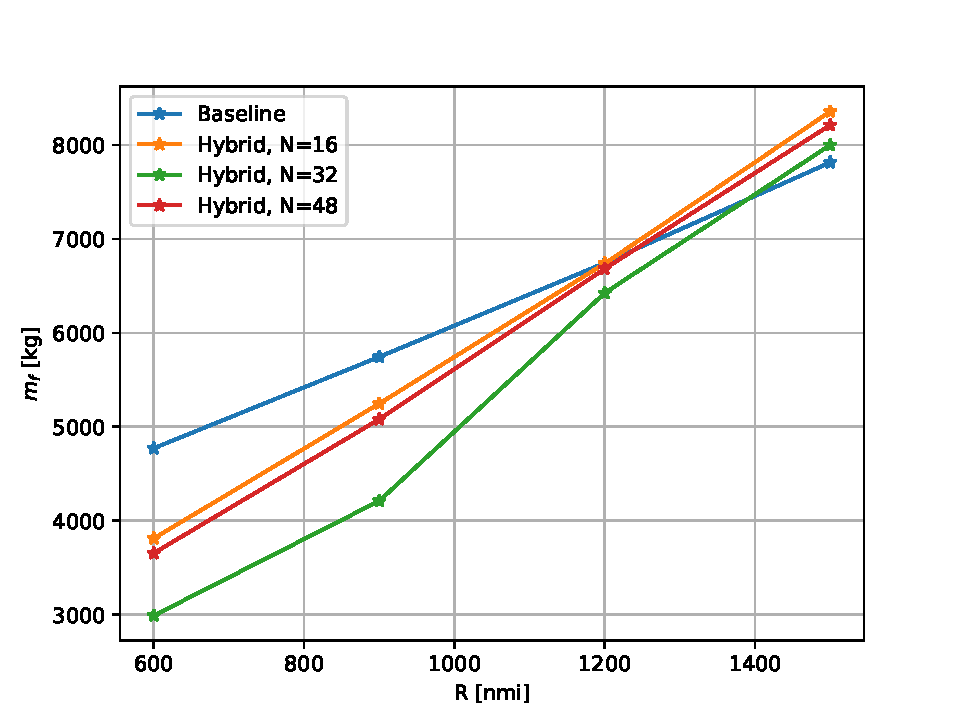
\includegraphics[keepaspectratio, width=0.6\textwidth]{images/chap4/bwb_hybrid_dep_optim_mf_comp}
	\caption{Fuel consumption as function of design range, comparison between the optimised baseline and the BWB with distributed electric propulsion. Three configurations have been analysed, corresponding to $N_{EM}=16,32,48$.}
	\label{fig:bwb_hybrid_dep_optim_mf_comp}
\end{figure}
\begin{figure}[!h]
	\centering
	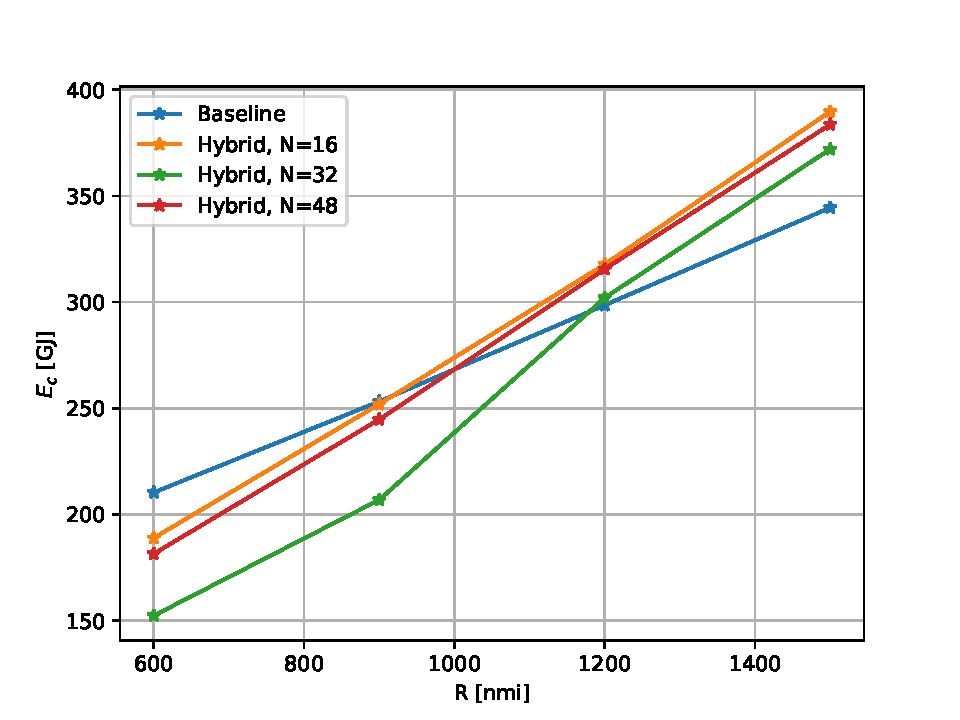
\includegraphics[keepaspectratio, width=0.6\textwidth]{images/chap4/bwb_hybrid_dep_optim_ec_comp}
	\caption{Energy consumption as function of design range, comparison between the optimised baseline and the BWB with distributed electric propulsion. Three configurations have been analysed, corresponding to $N_{EM}=16,32,48$.}
	\label{fig:bwb_hybrid_dep_optim_ec_comp}
\end{figure}
\begin{figure}[!h]
	\centering
	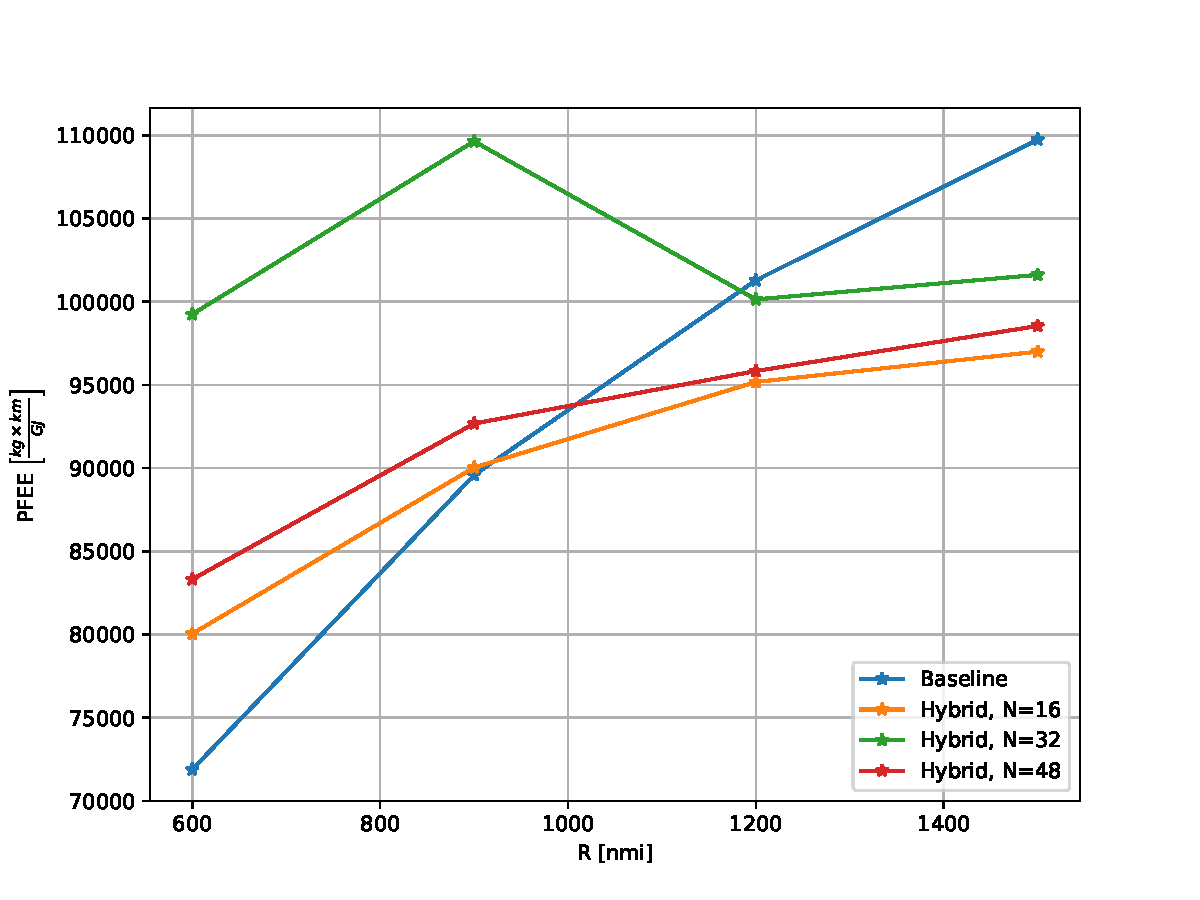
\includegraphics[keepaspectratio, width=0.6\textwidth]{images/chap4/bwb_hybrid_dep_optim_pfee_comp}
	\caption{PFEE, defined in Eq.~\eqref{eq:pfee} as function of design range, comparison between the optimised baseline and the BWB with distributed electric propulsion. Three configurations have been analysed, corresponding to $N_{EM}=16,32,48$.}
	\label{fig:bwb_hybrid_dep_optim_pfee_comp}
\end{figure}
Complementary to the figures, Table~\ref{tab:bwb_hybrid_dep_optim_res_n16}, Table~\ref{tab:bwb_hybrid_dep_optim_res_n32} and Table~\ref{tab:bwb_hybrid_dep_optim_res_n48} report values for parameters of interest for the cases with 16, 32 and 48 engines respectively.
\begin{table}[!h]
	\centering
	\begin{tabular}{l l c c c c}
		\cline{3-6}
		& & \multicolumn{4}{c}{\textbf{Range} [nmi]} \\
		& & \textbf{600} & \textbf{900} & \textbf{1200} & \textbf{1500} \\
		\hline
		\textbf{MTOW} & [\si{\tonne}] & 83.8 & 85.9 & 87.6 & 91.3 \\
		\textbf{OWE} & [\si{\tonne}] & 65.6 & 67.1 & 68.3 & 69.3 \\
		\textbf{Wing area} & [\si{\square\meter}] & 385.83 & 388.54 & 389.98 & 399.84 \\
		\textbf{Max. LoD} & & 24.02 & 23.89 & 23.88 & 23.83  \\
		\textbf{Battery volume} & [\si{\cubic\meter}] & 1.3 & 1.83 & 2.02 & 2.26 \\
		\textbf{FPR} & & 1.38 & 1.40 & 1.37 & 1.40 \\
		\textbf{Fuel mission} & [\si{\tonne}] & 3.81 & 5.25 & 6.74 & 8.36 \\
		\textbf{Energy consumption} & [\si{\giga\joule}] & 188.90 & 251.92 & 317.74 & 389.71 \\
		\hline
		\textbf{CAT.POL.A.410(a)-1} & [ft\si{\per\minute}] & 1534.40 & 1553.15 & 1490.01 & 1351.26 \\
		\textbf{CAT.POL.A.410(a)-2} & [ft\si{\per\minute}] & 2012.61 & 1971.61 & 1643.13 & 1524.97 \\
		\textbf{CS-25.119(a)} & [\%] & 9.13 & 10.03 & 10.01 & 9.61 \\
		\textbf{CS-25.121(a)} & [\%] & 10.91 & 14.92 & 14.56 & 13.45 \\
		\textbf{CS-25.121(b)} & [\%] & 2.42 & 2.64 & 2.42 & 2.68 \\
		\textbf{CS-25.121(c)} & [\%] & 10.91 & 9.82 & 14.55 & 13.42 \\
		\textbf{CS-25.121(d)} & [\%] & 8.01 & 8.98 & 8.96 & 8.43 \\
		\hline
	\end{tabular}
	\caption{Quantities of interest for the optimised BWB with distributed electric ducted fan, $N_{EM}=16$.}
	\label{tab:bwb_hybrid_dep_optim_res_n16}
\end{table}
\begin{table}[!h]
	\centering
	\begin{tabular}{l l c c c c}
		\cline{3-6}
		& & \multicolumn{4}{c}{\textbf{Range} [nmi]} \\
		& & \textbf{600} & \textbf{900} & \textbf{1200} & \textbf{1500} \\
		\hline
		\textbf{MTOW} & [\si{\tonne}] & 90.7 & 91.3 & 91.9 & 93.4 \\
		\textbf{OWE} & [\si{\tonne}] & 74.1 & 75.3 & 76.9 & 78.3 \\
		\textbf{Wing area} & [\si{\square\meter}] & 390.53 & 391.28 & 398.53 & 399.98 \\
		\textbf{Max. LoD} & & 23.43 & 23.39 & 23.02 & 23.01 \\
		\textbf{Battery volume} & [\si{\cubic\meter}] & 1.27 & 1.48 & 1.69 & 1.77 \\
		\textbf{FPR} & & 1.15 & 1.16 & 1.19 & 1.21 \\
		\textbf{Fuel mission} & [\si{\tonne}] & 2.99 & 4.21 & 6.42 & 8.01 \\
		\textbf{Energy consumption} & [\si{\giga\joule}] & 152.35 & 206.87 & 302.00 & 372.02 \\
		\hline
		\textbf{CAT.POL.A.410(a)-1} & [ft\si{\per\minute}] & 2012.61 & 1971.61 & 1643.13 & 1524.97 \\
		\textbf{CAT.POL.A.410(a)-2} & [ft\si{\per\minute}] & 1337.96 & 1334.37 & 1395.39 & 1393.73 \\
		\textbf{CS-25.119(a)} & [\%] & 10.84 & 10.82 & 12.25 & 12.05 \\
		\textbf{CS-25.121(a)} & [\%] & 22.62 & 22.29 & 17.54 & 18.28 \\
		\textbf{CS-25.121(b)} & [\%] & 2.46 & 2.59 & 2.51 & 2.83 \\
		\textbf{CS-25.121(c)} & [\%] & 22.51 & 22.19 & 17.54 & 18.27 \\
		\textbf{CS-25.121(d)} & [\%] & 9.65 & 9.63 & 11.05 & 10.84 \\
		\hline
	\end{tabular}
	\caption{Quantities of interest for the optimised BWB with distributed electric ducted fan, $N_{EM}=32$.}
	\label{tab:bwb_hybrid_dep_optim_res_n32}
\end{table}
\begin{table}[!h]
	\centering
	\begin{tabular}{l l c c c c}
		\cline{3-6}
		& & \multicolumn{4}{c}{\textbf{Range} [nmi]} \\
		& & \textbf{600} & \textbf{900} & \textbf{1200} & \textbf{1500} \\
		\hline
		\textbf{MTOW} & [\si{\tonne}] & 91.4 & 93.5 & 95.7 & 98.1 \\
		\textbf{OWE} & [\si{\tonne}] & 74.1 & 74.8 & 75.4 & 76.3 \\
		\textbf{Wing area} & [\si{\square\meter}] & 340.42 & 340.38 & 341.81 & 341.76 \\
		\textbf{Max. LoD} & & 25.18 & 25.15 & 25.08 & 24.78 \\
		\textbf{Battery volume} & [\si{\cubic\meter}] & 1.47 & 1.65 & 1.99 & 2.08 \\
		\textbf{FPR} & & 1.26 & 1.27 & 1.29 & 1.29 \\
		\textbf{Fuel mission} & [\si{\tonne}] & 3.65 & 5.08 & 6.68 & 8.21 \\
		\textbf{Energy consumption} & [\si{\giga\joule}] & 181.48 & 244.73 & 315.56 & 383.61 \\
		\hline
		\textbf{CAT.POL.A.410(a)-1} & [ft\si{\per\minute}] & 1553.11 & 1478.16 & 1360.73 & 1279.13 \\
		\textbf{CAT.POL.A.410(a)-2} & [ft\si{\per\minute}] & 1684.02 & 1678.41 & 1586.46 & 1471.59 \\
		\textbf{CS-25.119(a)} & [\%] & 9.49 & 9.42 & 9.38 & 9.77 \\
		\textbf{CS-25.121(a)} & [\%] & 12.53 & 12.60 & 13.36 & 13.64 \\
		\textbf{CS-25.121(b)} & [\%] & 2.52 & 2.83 & 2.89 & 2.90 \\
		\textbf{CS-25.121(c)} & [\%] & 12.56 & 12.62 & 13.41 & 13.68 \\
		\textbf{CS-25.121(d)} & [\%] & 8.39 & 8.31 & 8.29 & 8.19 \\
		\hline
	\end{tabular}
	\caption{Quantities of interest for the optimised BWB with distributed electric ducted fan, $N_{EM}=48$.}
	\label{tab:bwb_hybrid_dep_optim_res_n48}
\end{table}

Results can be compared with that shown in Table~\ref{tab:a320_2035_optim_res}. 
Both for the fuel and the energy consumption, the evidence of a ``breakdown range'' exists, and as in previous case, it is shifted to the left considering the energy. 
In all the cases, the zone of interest for the design is increased with respect to the hybrid BWB (see Fig.~\ref{fig:hybrid_dep_optim_mf_comp}, Fig.~\ref{fig:hybrid_dep_optim_ec_comp} and Fig.~\ref{fig:hybrid_dep_optim_pfee_comp}).
Curves are not linear, because of the effect of the FPR, which is more significant in the case with 32 engines. 

Also, the configuration with $N_{EM}=32$ is the most performing one, since it represents a balance between aerodynamics and propulsive efficiency. 
Considering the PFEE, the range breakdown is about 1200~nmi, compared to 900 of hybrid TAW; $N_{EM}=16$ and $N_{EM}=48$ have similar performance, and the range breakdown is about 800~nmi. 
It is also interesting to note that the case with 32 engines shows a maximum for PFEE on a range of 900~nmi approximately.

However, the case with $N=48$ shows an interesting behavior.
The global minimum configuration is represented by the case with maximum LoD, and indeed Table~\ref{tab:bwb_hybrid_dep_optim_res_n48} shows that its value is higher than other cases. 
This result is explained considering that, when the number of engines increases, the MTOW does the same; for this configuration, penalties in weight are so relevant that the aircraft is not capable anymore to climb, and then it finds the path to reduce weight in order to reduce batteries and ease the climb. 

The mass breakdown, for the case with 32 engines and a range of 900~nmi the mass breakdown, is provided in Fig.~\ref{fig:bwb_hybrid_dep_mb}, with the global overlook on the left and details of airframe breakdown on the right.
\begin{figure}[!h]
	\centering
	\begin{subfigure}{0.45\textwidth}
		\centering
		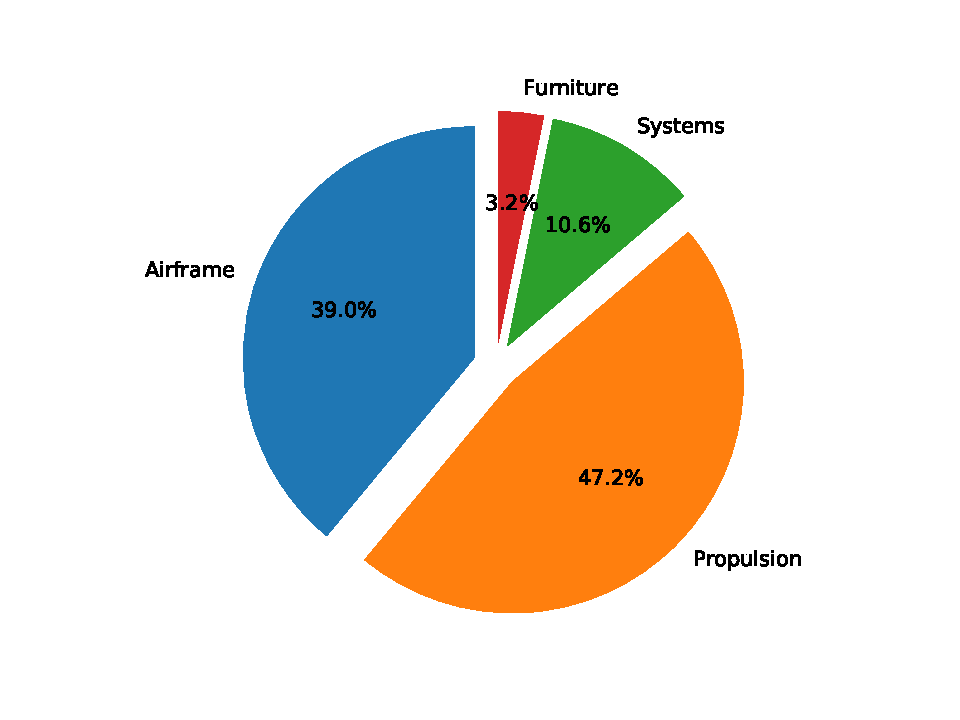
\includegraphics[keepaspectratio, width=\linewidth]{images/chap4/bwb_hybrid_dep_mb}
		\caption{Global breakdown.}
		\label{fig:bwb_hybrid_dep_mb_global}
	\end{subfigure}
	\begin{subfigure}{0.45\textwidth}
		\centering
		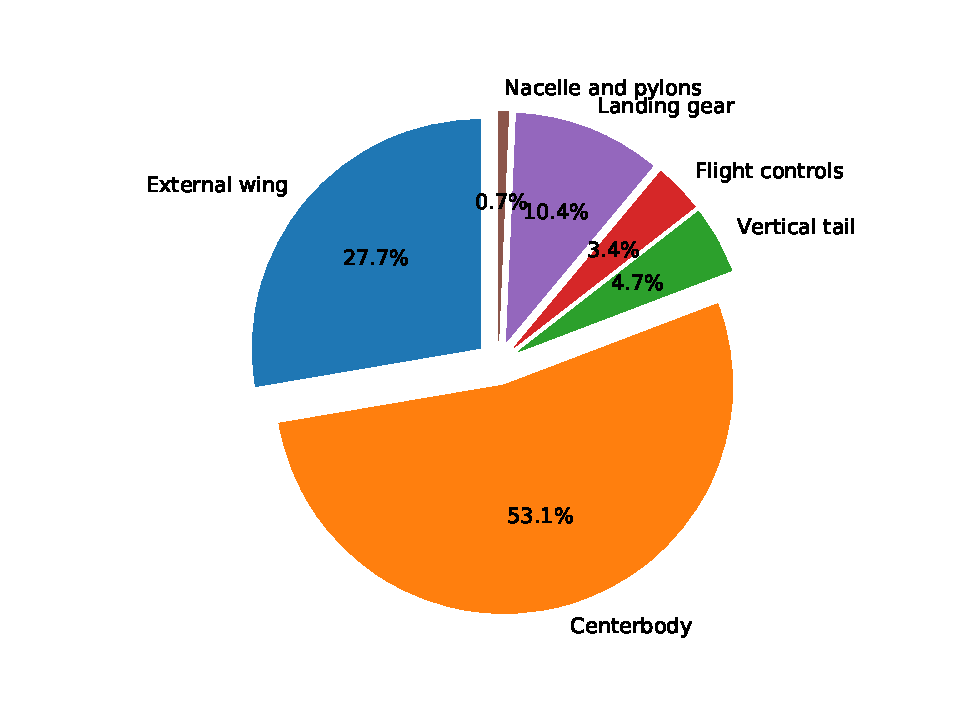
\includegraphics[keepaspectratio, width=\linewidth]{images/chap4/bwb_hybrid_dep_airframe_mb}
		\caption{Airframe detail.}
		\label{fig:bwb_hybrid_dep_mb_detail_airframe}
	\end{subfigure}
	\caption{Mass breakdown for the BWB with distributed electric propulsion, $N_{EM}=32$, R=900~nmi. Mass norm is the revised French 2001/D for hybrid architectures, used in FAST~\cite{bib:mass_breakdown}.}
	\label{fig:bwb_hybrid_dep_mb}
\end{figure}
Compared to the case with conventional engines shown in Fig.~\ref{fig:bwb_conv_mb}, the airframe contribution is almost halfed whereas the propulsion contribution is more than doubled. 
This is mainly due to the presence of batteries, that again introduce the most relevant penalty in weight. 
Concerning the airframe division, because of the heavier MTOW the centerbody accounts for the 58\% compared to 55\% of previous case, but generally the order of magnitude does not change. 
It is useful to recall that cabin weight depends on the MTOW as described in Eq.~\eqref{eq:bwb_cabin_mass}, which explains the higher percentage. 

Concerning the certification part, all the configurations comply with the proposed revised CS-25 for the hybrid propulsion. 
The top of climb and top of descent conditions are taken with a great margin; the most stringent one is the OCI condition at 400~ft. 
To assess the difference considering more margin on the minimum condition suggested by certification, a new optimisation is carried out, considering the case with 32 engines and range of 900~nmi. 
For this simulation, the lower limits of certification are taken as the A320 test case, reported in Table~\ref{tab:fast_base_ccm}. 
The difference in fuel consumption is of 100~\si{\kilogram}, because the power required is of course higher, and this increases the weight. 
However, the oversizing is in the order of 2.5~\si{\mega\watt}, since all the other conditions have already margin with respect to Table~\ref{tab:fast_base_ccm}.
Detailed comparison is reported in Table~\ref{tab:bwb_hybrid_dep_optim_ccm_comp}. 
\begin{table}[!h]
	\centering 
	\begin{tabular}{l l c c}
		\cline{3-4}
		& & \textbf{CS-25 limit} & \textbf{A320 2005 limit} \\
		\hline
		\textbf{MTOW} & [\si{\kilogram}] & 91277.08 & 91426.52 \\
		\textbf{Power @ 400ft} & [\si{\mega\watt}] & 8.73 & 11.22 \\
		\textbf{Battery volume} & [\si{\cubic\meter}] & 1.48 & 1.49 \\
		\textbf{Fuel consumption} & [\si{\kilogram}] & 4216 & 4330 \\
		\hline
	\end{tabular}
	\caption{Comparison between the two BWB with DEP optimisation problems, considering the CCM lower limit as specified in the CS-25~\cite{bib:cs25} and equals to the A320 2005 version, reported in Table~\ref{tab:fast_base_ccm}. $N_{EM}=32$, R~=~900~nmi case.}
	\label{tab:bwb_hybrid_dep_optim_ccm_comp}
\end{table} 
However, this assessment is useful since a more refined design may take a safety limit than the minimum values of CS specifications. 

Next section will present the Pareto frontier, comparing the results between a gradient free and a gradient based method. 

\subsection{Pareto frontier for the proposed BWB concept}
\label{subsec:chap4_bwb_pareto}

The Pareto frontier is obtained in similar manner than has been done in Sec.~\ref{subsubsec:chap3_hybrid_pareto}. 
The two objective functions are the energy consumption $E_c$ and the OWE $m_e$, which are related to costs. 
The genetic algorithm NSGA-II, which is an algorithm capable to tackle the multiobjective optimisation, is compared with SNOPT, that uses gradient. 
In mathematical notation, the problem assumes the following form: 
\begin{equation*}
	\left\{\begin{array}{l l}
		\textrm{minimise } & \underline{f}\left(\underline{x}\right)=\left[m_e, E_c\right]\in\mathbb{R}^{2} \\
		\textrm{with respect to } & \underline{x}\in\mathbb{R}^{18} \\
		\textrm{subject to } & \underline{c}\left(\underline{x}\right)\in\mathbb{R}^{18} \\						 
	\end{array}\right.
\end{equation*}
with $\underline{f}\left(\underline{x}\right)=\left[m_e, E_c\right]$, $\underline{x}$ and $\underline{c}\left(\underline{x}\right)$ defined in Table~\ref{tab:bwb_hybrid_dep_problem_optimisation_definition}. 
In the case of SNOPT the auxiliary function defined in Eq.~\eqref{eq:multiobj_aux_func} is used: varying the parameter $\alpha$ in the range $\hbox{[0,1]}$ all the points are exploited. 
In this case, the problem can be written as
\begin{equation*}
	\left\{\begin{array}{l l}
		\textrm{minimise } & f\left(\underline{x}, \alpha\right)\in\mathbb{R}  \\
		\textrm{with respect to } & \underline{x}\in\mathbb{R}^{18} \\
		\textrm{subject to } & \underline{c}\left(\underline{x}\right)\in\mathbb{R}^{18} \\						 
	\end{array}\right.
\end{equation*}
with $f\left(\underline{x}\right)$ defined from Eq.~\eqref{eq:multiobj_aux_func} and $\alpha\in[0,1]$.

The case considered for the Pareto frontier is the configuration with 32 engines, with a range of 900~nmi; problem is the same of Table~\ref{tab:bwb_hybrid_dep_problem_optimisation_definition} with two objectives in place of one. 
The exploration points used by NSGA-II are shown in Fig.~\ref{fig:bwb_hybrid_dep_pareto_exploration}, where feasible points are marked in blue, meanwhile points belonging to Pareto frontier in red. 
Compared to previous case of the hybrid TAW optimisation, 20000 points have not been sufficient to obtain a smooth Pareto, thus the number of points is increased until good results were obtained. 
At the end, 50000 points have been explored.
\begin{figure}[!h]
	\centering
	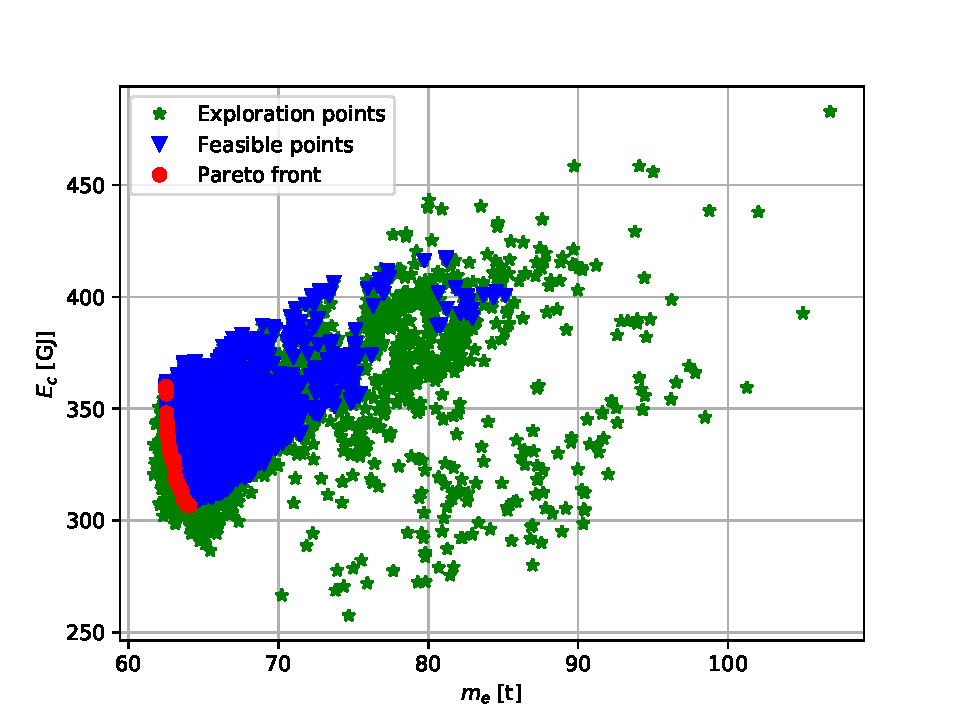
\includegraphics[keepaspectratio, width=0.6\textwidth]{images/chap4/bwb_exp_pt}
	\caption{Exploration points using NSGA-II, for the multiobjective optimisation of BWB with distributed electric propulsion, $N_{EM}=32$ and R=~900~nmi. 50000 points considered.}
	\label{fig:bwb_hybrid_dep_pareto_exploration}
\end{figure}
The higher number of points results in a computational cost of about 85~\si{\hour}, confirming the high demand required by such algorithm. 

The comparison between the Pareto frontier obtained with NSGA-II and SNOPT is shown in Fig.~\ref{fig:bwb_hybrid_dep_pareto}: visually the two curves are comparable each others, in fact differences are small, and are due to numerical approximation. 
\begin{figure}[!h]
	\centering
	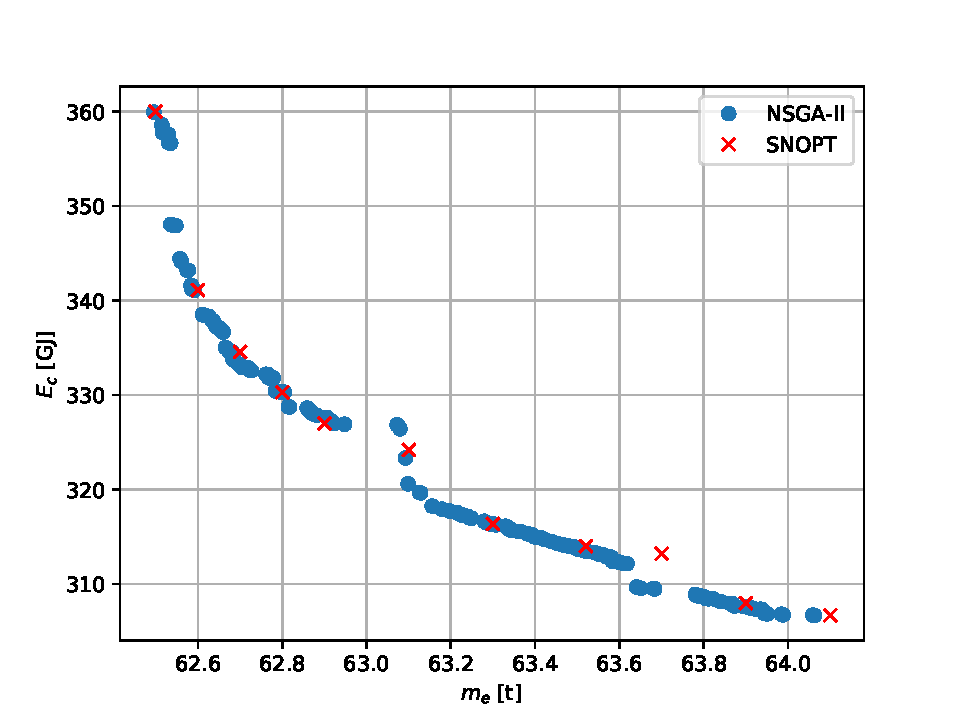
\includegraphics[keepaspectratio, width=0.6\textwidth]{images/chap4/bwb_pareto}
	\caption{Comparison between the Pareto frontier obtained with NSGA-II and SNOPT, through the auxiliary function in Eq.~\eqref{eq:multiobj_aux_func}. BWB with DEP case, $N_{EM}=32$ and R~=~900~nmi.}
	\label{fig:bwb_hybrid_dep_pareto}
\end{figure}
To better assess the difference between the two methods, the $\mathcal{L}_2$-norm for the final objective function and design variable is computed and results are in Table~\ref{tab:bwb_hybrid_dep_pareto_norm_l2}.
\begin{table}[!h]
	\centering
	\begin{tabular}{l c}
		\hline
		$\Vert\underline{f}^{*}_{SNOPT} - \underline{f}^{*}_{NSGAII}\Vert_2$ & $6.84\times10^{-6}$ \\
		$\Vert\underline{x}^{*}_{SNOPT} - \underline{x}^{*}_{NSGAII}\Vert_2$ & $4.49\times10^{-5}$ \\
		\hline
	\end{tabular}
	\caption{$\mathcal{L}_2$-norm calculation between the final objective function and design variable vectors. The subscript identifies the method.}
	\label{tab:bwb_hybrid_dep_pareto_norm_l2}
\end{table}

Because of the existance of local minima, multipoint approach must be used for SNOPT simulations in this case too to ensure to get the global minimum, for each point. 
However, knowing where is the final solution, the initial point can be taken around the point, reducing the computational cost and eventually also the number of initial points. 
In total, for each $\alpha$ 5 different $x^{(0)}$ are considered; in mean the time for a simulation is about 30~\si{\minute}, so finally the global computational time is about 25~\si{\hour} for the $11\times10$ simulation. 

In this case too the cost is higher than previous case, but the difference between the two approaches is still of about 60\%; also it is to not forget that all the points can be run at same time, so a Pareto can be obtained in about 3~\si{\hour}. 
It is then confirmed that the gradient-based methods are more efficient than the gradient-free. 

\subsection{Results for an hybrid BWB concept without batteries}
\label{subsec:chap4_bwb_hybrid_without_batteries}

This section exploits a particular case of BWB, where the electric power is supplied solely by the two turbogenerators. 
Indeed, since from the analysis of the hybrid TAW it has been noted that the penalties in weight introduced by batteries are so relevant to drastically impact the fuel and energy consumption.
This has been confirmed also by the mission optimisation carried out in Sec.~\ref{subsec:chap3_hybrid_expl_optim}, where from the results is more convenient to remove batteries for fuel saving. 
These elements have been introduced by to satisfy the TLAR of zero emissions up to 3000~ft.
However, fostered by previous results and other similar concepts in literature, like the DRAGON~\cite{bib:dragon} or the N3-X~\cite{bib:kim_n3x_2008}, it has been decided to analyse the BWB aircraft where only the generators supply electric power.
The analysis is also useful since the batteries' technology has the most uncertainty, and in case the values assumed here will not be available, another solution is studied. 

To estimate the impact of absence of batteries, the same optimal configurations are considered; so at this stage no optimisation is done. 
Results in terms of fuel consumption are shown in Fig.~\ref{fig:bwb_hybrid_dep_gen_optim_mf_comp}.
Since there is only one single source power, show the energy consumption and the PFEE curves is pointless, because they are simply scaled with respect to fuel consumption.
\begin{figure}[!h]
	\centering
	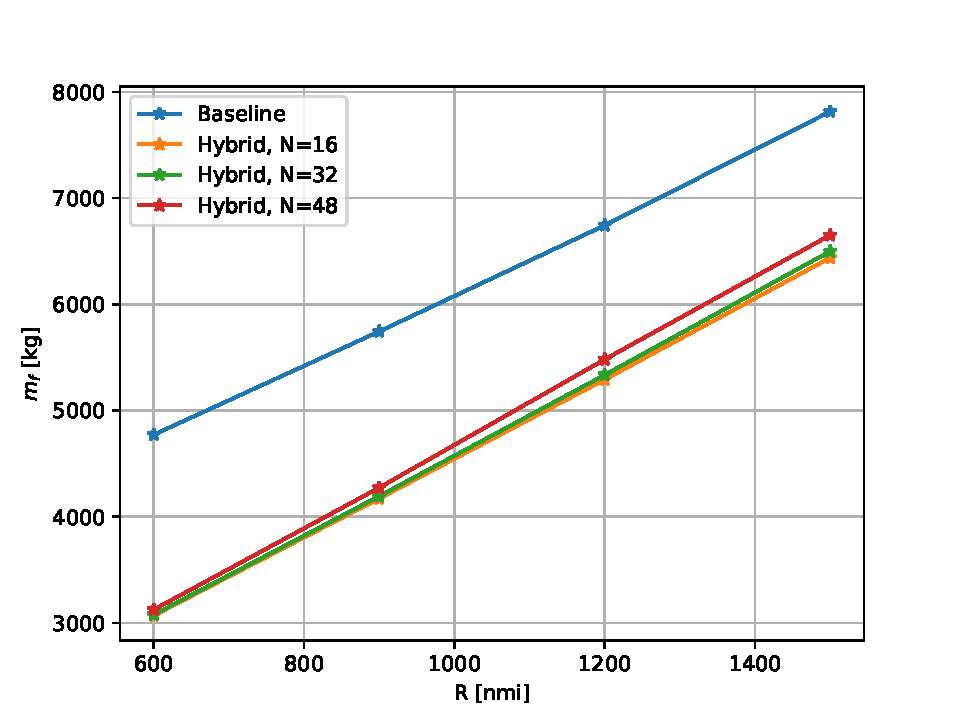
\includegraphics[keepaspectratio, width=0.6\textwidth]{images/chap4/bwb_hybrid_gen_optim_mf_comp}
	\caption{Fuel consumption as function of design range, comparison between the optimised baseline and the BWB with DEP, where the electric propulsion is obtained by turbogenerators solely.}
	\label{fig:bwb_hybrid_dep_gen_optim_mf_comp}
\end{figure}
Table~\ref{tab:bwb_hybrid_dep_gen_optim_res_n16}, Table~\ref{tab:bwb_hybrid_dep_gen_optim_res_n32} and Table~\ref{tab:bwb_hybrid_dep_gen_optim_res_n48} report the quantities of interest for this case, with 16, 32 and 48 engines respectively. 
\begin{table}[!h]
	\centering
	\begin{tabular}{l l c c c c}
		\cline{3-6}
		& & \multicolumn{4}{c}{\textbf{Range} [nmi]} \\
		& & \textbf{600} & \textbf{900} & \textbf{1200} & \textbf{1500} \\
		\hline
		\textbf{MTOW} & [\si{\tonne}] & 68.6 & 69.8 & 71.0 & 72.3 \\
		\textbf{OWE} & [\si{\tonne}] & 51.9 & 52.0 & 52.1 & 52.2 \\
		\textbf{Max. LoD} & & 25.59 & 25.56 & 25.54 & 25.51  \\
		\textbf{Fuel mission} & [\si{\tonne}] & 3.07 & 4.17 & 5.29 & 6.44 \\
		\hline
		\textbf{CAT.POL.A.410(a)-1} & [ft\si{\per\minute}] & 2240.91 & 2168.93 & 2098.28 & 2028.51 \\
		\textbf{CAT.POL.A.410(a)-2} & [ft\si{\per\minute}] & 762.37 & 760.50 & 758.61 & 756.66 \\
		\textbf{CS-25.119(a)} & [\%] & 14.29 & 14.27 & 14.24 & 14.22 \\
		\textbf{CS-25.121(a)} & [\%] & 13.57 & 13.06 & 12.54 & 12.69 \\
		\textbf{CS-25.121(b)} & [\%] & 11.98 & 11.69 & 11.42 & 11.14 \\
		\textbf{CS-25.121(c)} & [\%] & 13.50 & 12.99 & 12.49 & 12.64 \\
		\textbf{CS-25.121(d)} & [\%] & 13.24 & 13.21 & 13.19 & 13.16 \\
		\hline
	\end{tabular}
	\caption{Quantities of interest for the BWB with distributed electric ducted fan, power supplied by turbogenerators solely, $N_{EM}=16$.}
	\label{tab:bwb_hybrid_dep_gen_optim_res_n16}
\end{table}
\begin{table}[!h]
	\centering
	\begin{tabular}{l l c c c c}
		\cline{3-6}
		& & \multicolumn{4}{c}{\textbf{Range} [nmi]} \\
		& & \textbf{600} & \textbf{900} & \textbf{1200} & \textbf{1500} \\
		\hline
		\textbf{MTOW} & [\si{\tonne}] & 69.9 & 71.2 & 72.5 & 73.8 \\
		\textbf{OWE} & [\si{\tonne}] & 53.3 & 53.4 & 53.5 & 53.7 \\
		\textbf{Max. LoD} & & 25.61 & 25.62 & 25.59 & 25.56  \\
		\textbf{Fuel mission} & [\si{\tonne}] & 3.08 & 4.19 & 5.33 & 6.50 \\
		\hline
		\textbf{CAT.POL.A.410(a)-1} & [ft\si{\per\minute}] & 2163.94 & 2093.61 & 2024.31 & 1955.93 \\
		\textbf{CAT.POL.A.410(a)-2} & [ft\si{\per\minute}] & 766.39 & 764.31 & 762.21 & 760.04 \\
		\textbf{CS-25.119(a)} & [\%] & 14.00 & 13.98 & 13.95 & 13.93 \\
		\textbf{CS-25.121(a)} & [\%] & 12.97 & 12.46 & 12.62 & 12.11 \\
		\textbf{CS-25.121(b)} & [\%] & 11.67 & 11.39 & 11.11 & 10.84 \\
		\textbf{CS-25.121(c)} & [\%] & 12.92 & 12.41 & 12.57 & 12.07 \\
		\textbf{CS-25.121(d)} & [\%] & 12.95 & 12.92 & 12.89 & 12.87 \\
		\hline
	\end{tabular}
	\caption{Quantities of interest for the BWB with distributed electric ducted fan, power supplied by turbogenerators solely, $N_{EM}=32$.}
	\label{tab:bwb_hybrid_dep_gen_optim_res_n32}
\end{table}
\begin{table}[!h]
	\centering
	\begin{tabular}{l l c c c c}
		\cline{3-6}
		& & \multicolumn{4}{c}{\textbf{Range} [nmi]} \\
		& & \textbf{600} & \textbf{900} & \textbf{1200} & \textbf{1500} \\
		\hline
		\textbf{MTOW} & [\si{\tonne}] & 72.1 & 73.4 & 74.8 & 76.1 \\
		\textbf{OWE} & [\si{\tonne}] & 55.4 & 55.5 & 55.7 & 55.8 \\
		\textbf{Max. LoD} & & 25.55 & 25.53 & 25.50 & 25.47  \\
		\textbf{Fuel mission} & [\si{\tonne}] & 3.12 & 4.27 & 5.48 & 6.65 \\
		\hline
		\textbf{CAT.POL.A.410(a)-1} & [ft\si{\per\minute}] & 2046.94 & 1978.26 & 1908.70 & 1843.54 \\
		\textbf{CAT.POL.A.410(a)-2} & [ft\si{\per\minute}] & 765.51 & 763.92 & 762.23 & 760.60 \\
		\textbf{CS-25.119(a)} & [\%] & 13.58 & 13.56 & 13.53 & 13.51 \\
		\textbf{CS-25.121(a)} & [\%] & 12.76 & 12.26 & 11.73 & 11.87 \\
		\textbf{CS-25.121(b)} & [\%] & 11.19 & 10.91 & 10.63 & 10.37 \\
		\textbf{CS-25.121(c)} & [\%] & 12.70 & 12.20 & 11.68 & 11.81 \\
		\textbf{CS-25.121(d)} & [\%] & 12.53 & 12.50 & 12.47 & 12.45 \\
		\hline
	\end{tabular}
	\caption{Quantities of interest for the BWB with distributed electric ducted fan, power supplied by turbogenerators solely, $N_{EM}=48$.}
	\label{tab:bwb_hybrid_dep_gen_optim_res_n48}
\end{table}

Results show the absence of batteries reduces the MTOW of about 30~\si{\tonne}, saving approximately 1.5~\si{\tonne} of fuel. 
The concept is always more performing than the A320 baseline on the set of design ranges of interest; also the three configurations varying the number of engines are very similar among them. 
%Considering a linear law, it is possible to extrapolate the range breakdown from Fig.~\ref{fig:bwb_hybrid_dep_gen_optim_mf_comp}, which results approximately 2200~nmi. 
It is also to note that the maximum LoD is higher in this case too: thanks to the lighter aircraft, the thrust at top of climb, which is the sizing condition for the ducted fan, is smaller. 
As main effect, the ducted fans are smaller too, and the reduction in wetted surface makes the aerodynamics better. 

On the certification side, all the conditions are respected with a great margin, both considering the limits from CS document and the A320 2005 version. 

In conclusion, for hybrid propulsion it is more convenient to limit or even remove the batteries, unless it is stricly necessary, as in the case of this research where the goal was to have zero emission in the atmospheric boundary layer. 

\section{Conclusions}
\label{sec:chap4_conclusion}

This chapter has the scope to define a procedure for the BWB sizing. 
The methodology adopted, that uses high fidelity on a common geometry to find methods suitable for conceptual design, allows to revise the sizing procedure with disciplines tailored for the BWB. 

After these analyses aerodynamic, mass models have been adapted to the problem; and also the contribution coming from the nacelle integration and the BLI is estimated.
Some details regarding boarding, evacuation, subsystems positioning and other aspects related to operations have also been discussed. 
Even if these aspects are not directly included in the conceptual sizing process, since they belong to another level of refinement, the discussion has been necessary to limit the risk of acceptance and feasibility (with respect to certification) of the proposed concept. 

The assumptions done are acceptable for the conceptual design, but of course they open new perspectives for a more detailed design. 
In particular, these issues are noted for further developments:
\begin{enumerate}
	\item CFD optimisation for airfoil shape;
	
	\item Lateral stability and control, for the elevons positioning and sizing;
	
	\item Proper evacuation simulation, to ensure that aircraft is emptied in 180~\si{\second} as requested by certification;
	
	\item Estimation of the surface needed for cargo doors and cutoffs for batteries, PMU and electrical components;
	
	\item Impact of operations on the design (\textit{i.e.} the cutoffs weaken the structure, and they have an impact on mass);
	
	\item Maintenance cost estimation.
\end{enumerate}

Once that the methodology has been defined, performances of a BWB architecture have been evaluated. 
At first, just a sizing has been carried out considering a BWB architecture mounting conventional high BPR engines. 
This analysis has been helpful in order to test the models adopted, separating the ones related to BWB from the ones specific for distributed electric propulsion. 
Results show that, due to the more complex architecture, BWB is heavier than a conventional aircraft, especially because of the cabin which is a relevant source of weight. 
Nevertheless, the benefits coming from the better aerodynamics counterbalance this drawback and in the end the BWB saves about 20\% of fuel, compared to conventional aircraft, on the same technology horizon. 
The tradeoff on operational missions shows instead that the BWB is very efficient in cruise, but the same is not true for other phases, and loss its advantage at very short range, where the cruise is not so long. 
Ferry range is of course increased because of the aerodynamics, and it may be ulteriorly augmented considering auxiliary tanks in the centerbody. 

Then the study is proceeded with the exploration of the BWB featuring DEP, in a similar way as done in Chapter~\ref{chap3:hybrid_dep_exploration} for the TAW concept mounting DEP. 
Starting from the sensitivity analysis it emerges that the most predominant parameters for performances are the ones that impact aerodynamics, confirming the assumption of very aerodynamically efficient concept. 
The optimisation results show that, in the limit of our model, the interaction between the disciplines leads to two different minima: a local one, corresponding to the most efficient cruise but worse performance in climb and descent, and a global one which is the best balance to reduce energy consumption in all phases. 

Similarly to the case of TAW aircraft a range breakdown is detected, despite it is greater than the previous case. 
In terms of energy, it was approximately 900~nmi, againt 1400~nmi for the BWB architecture. 
It is clear that the presence of batteries, that account for about 14~\si{\tonne}, is penalising, in spite of the advantage of zero emission close to ground. 
For this reason, the same configurations have been studied considering the hybrid propulsion generated solely by the two turbogenerators. 
In this case performances are improved and the BWB is always more performing than the conventional aircraft in the range of interest (between 600 and 1500~nmi).
The breakdown value is extrapolated and it results about 2200~nmi. 

Finally, in this case too the Pareto frontier is obtained, showing the tradeoff between OWE and energy consumption. 
For this case, the genetic algorithm NSGA-II required 50000 points to have a smooth curve; however also SNOPT needed more time because the multistart approach must be used, to avoid the presence of local minima. 
In any case, the use of gradients speeds up the generation of Pareto of about 60\%, in agreement with the other case of TAW aircraft featuring distributed propulsion. 

In conclusion, the MDO formulation developed through the research has been applied on the BWB with distributed electric propulsion test case, with results that confirm the goodness of these techniques for unconventional configurations. 
Despite the relatively low number of design variables (contained to 21), the interaction between disciplines is so strong with respect to the design problem for conventional aircraft that MDO is necessary to get the best tradeoff. 
Otherwise, the intuition may be misleading, as \textit{i.e.} in the case of the BWB, where surprisingly the configuration with best LoD value is not the optimal one. 

Regarding the case study itself, the BWB with DEP is one of the most promising concepts since it is naturally very aerodynamically efficient, and opens new technologies, like the BLI, in conjunction with hybrid propulsion. 
However, in case of double source energy, the batteries limit the zone of interest for the design, at least in the limit of the technological assumptions done within this reseach. 
The concept does the best when the power is generated simply by two turbogenerators. 

\clearpage

\begin{mdframed}[hidealllines=true,backgroundcolor=blue!20]
	\section*{Synthesis of the chapter}
	
	\begin{itemize}
		
		\item Conceptual design methods implemented in FAST or available in literature have been validated using high-fidelity analyses. 
		
		\item Off-design criteria are considered, such as the boarding and the subsystem displacements, in order to evaluate the acceptance of the concept. Suggestions for further development are given. 
		
		\item The Blended Wing-Body concept with conventional engines is first explored: 
		\begin{itemize}
			\item[-] On design mission it shows about 15\% fuel reduction compared to conventional aircraft. 
			
			\item[-] On operational missions the BWB is more performing on long range, whereas on short and very short range the reference aircraft is slightly better. The trend is explained because the BWB is not optimised for climb and descent segment, and it also flies at best altitude, thus when the cruise segment is reduced it loses its advantages. 
			
			\item[-] Payload-Range is larger than the conventional aircraft, showing that the BWB concept has an extended operational domain, which makes this concept more flexible to operations.
		\end{itemize}
	
		\item The Blended Wing-Body featuring distributed electric propulsion, objective of this research, is then evaluated: 
		\begin{itemize}
			\item[-] The optimisation finds more than one region of interest for the design of the BWB. The most efficient aerodynamics configuration does not represent the global minimum, but the overall optimum BWB is represented by a balanced configuration between propulsion and aerodynamics.
			
			\item[-] In agreement with the results of Chapter~\ref{chap3:hybrid_dep_exploration}, the concept shows a zone of interest for the design. However, it is enlarged compared to the previous case of hybrid tube-and-wing with distributed propulsion. 
			
			\item[-] The case with 32 engines is again the most performing, because it represents the best compromise between aerodynamics and propulsive efficiency. 
			
			\item[-] A simulation without batteries is carried out, since they represent the biggest penalty in mass. Results show that in case the electric power is produced solely by gasturbines the proposed concept is always more performing than the reference aircraft.
			
		\end{itemize}
		
		\item The Pareto frontier simulation confirms the reduction in computational cost of about 70\% with the utilisation of gradient's information. 
		
	\end{itemize}
	
\end{mdframed}

\clearpage

\begin{mdframed}[hidealllines=true,backgroundcolor=green!20]
	\section*{Research contribution }
	
	\begin{itemize}
		\item[-] \textbf{Conference}. EASN 2019 in Athens: presentation of the multifidelity approach and the BWB with distributed propulsion, in separate sessions. 
		
		\item[-] \textbf{Conference}. AEC 2020 in Bordeaux: presentation of the BWB with distributed propulsion, and related paper in the proceedings. 
		
		\item[-] \textbf{Conference paper}. A. Sgueglia, P. Schmollgruber, E. Benard, N. Bartoli and J. Morlier, \emph{Preliminary sizing of a medium range Blended Wing-Body using a Multidisciplinary Design Analysis approach}, MATEC Web of Conferences, Vol. 233, n. 14, 2018. DOI: \url{10.1051/matecconf/201823300014}	
		
		\item[-] \textbf{Journal paper}. A. Sgueglia, L. Cerquetani, L. C. e Chuna Lima, D. A. Kharoub, P. Rodriguez Otero, H. Kaur, P. Traverso, S. S. C. Yella and E. Benard, \emph{Multidisciplinary and multifidelity exploration of a medium range Blended Wing-Body transport aircraft}, Aerospace (submitted), 2019.
		
	\end{itemize}
\end{mdframed}